% \pdfoutput=1
\documentclass[nohyperref]{article}
% \usepackage{arxiv}

% hyperref makes hyperlinks in the resulting PDF.
% If your build breaks (sometimes temporarily if a hyperlink spans a page)
% please comment out the following usepackage line and replace
% \usepackage{icml2023} with \usepackage[nohyperref]{icml2023} above.

\usepackage[accepted]{icml2023}


\usepackage[utf8]{inputenc} % allow utf-8 input
\usepackage[T1]{fontenc}    % use 8-bit T1 fonts
\usepackage{hyperref}       % hyperlinks
%\usepackage[colorlinks=true,linkcolor=red]{hyperref}
\usepackage{xcolor}
\usepackage{url}            % simple URL typesetting
\usepackage{booktabs}       % professional-quality tables
\usepackage{nicefrac}       % compact symbols for 1/2, etc.
\usepackage{microtype}      % microtypography
\usepackage{soul}   % hyphenation for letter spacing, hyphenation, etc
%\usepackage{authblk}

%\pagestyle{headings}
\usepackage{mathtools}
\usepackage{tabularx}
\usepackage{graphicx}
\usepackage[normalem]{ulem}
\usepackage{xspace}
\usepackage{multirow}
% algorithm and algorithmic are included in the style file
%\usepackage{algorithm}
%\usepackage[noend]{algorithmic}
%\usepackage[noend]{algpseudocode}
%\usepackage{algorithm2e}
\usepackage{amsmath}
\usepackage{amssymb}
\usepackage{amsthm}
\usepackage{amsfonts}       % blackboard math symbols
\usepackage{wrapfig}
\usepackage{adjustbox}
\usepackage{multicol}
%\usepackage[font=small]{caption}
\usepackage{mwe}
%\showthe\baselineskip
\usepackage[inline, shortlabels]{enumitem}
\setlist[enumerate]{nosep}
%\baselineskip
\usepackage[capitalize,noabbrev]{cleveref}
% math and blackboard math symbols specified using \mathbbm{}. For example, \mathbbm{N} for the set of natural numbers
\usepackage{bm}
\usepackage{bbm}
\usepackage{array}
\usepackage{rotating}       % rotation of figures and tables
\usepackage{verbatim}
%\usepackage{float}      % Improves the interface for defining floating objects such as figures and tables
%\usepackage{subfig}
% \usepackage{subfigure}
\usepackage{caption}
\usepackage{subcaption}    % More recent compared to subfig
\usepackage{tcolorbox}

\DeclareGraphicsExtensions{.pdf, .png}
%\usepackage{pgf}
%\usepackage{epsf,psfig,epsfig}
%\usepackage{cite}       % Supports compressed, sorted lists of numerical citations, and also deals with various punctuation and other issues of representation
%\usepackage{slashbox}       % Tabular cells with diagonal lines in them

\newcommand*{\proposed}{{\tt proposed}\@\xspace}

\newcommand{\jihye}[1]{{\color{blue}[Jihye: #1]}}
\newcommand{\jayaram}[1]{\textcolor{red}{Jayaram: #1}}
\newcommand{\somesh}[1]{{\color{red}[Somesh]: #1]}}
\newcommand{\ryan}[1]{\textcolor{brown}{Ryan: #1}}
\newcommand{\atul}[1]{\textcolor{red}{Atul: #1}}


%%%%%%%%%%%%%%%%%%%%%%%%%%%%%%%%
% THEOREMS
%%%%%%%%%%%%%%%%%%%%%%%%%%%%%%%%
\theoremstyle{plain}
\newtheorem{theorem}{Theorem}
\newtheorem{proposition}[theorem]{Proposition}
\newtheorem{lemma}[theorem]{Lemma}
\newtheorem{corollary}[theorem]{Corollary}
\theoremstyle{definition}
\newtheorem{definition}[theorem]{Definition}
\newtheorem{assumption}[theorem]{Assumption}
\theoremstyle{remark}
\newtheorem{remark}[theorem]{Remark}

\newcommand{\BigO}[1]{\ensuremath{\operatorname{O}\left(#1\right)}}
\newcommand{\argmin}{\operatornamewithlimits{arg\!\min}}
\newcommand{\argmax}{\operatornamewithlimits{arg\!\max}}
%\renewcommand{\figurename}{Fig.}
%\newcommand{\proof}{\noindent {\bf Proof:\\}}
\newcommand{\ben}{\begin{enumerate}}
\newcommand{\een}{\end{enumerate}}
\newcommand{\beq}{\begin{equation}}
\newcommand{\eeq}{\end{equation}}
\newcommand{\beqa}{\begin{eqnarray}}
\newcommand{\eeqa}{\end{eqnarray}}
\newcommand{\bit}{\begin{itemize}}
\newcommand{\eit}{\end{itemize}}
\newcommand{\btab}{\begin{tabular}}
\newcommand{\etab}{\end{tabular}}
%\newcommand{\rr}{\raggedright}
%\newcommand{\tn}{\tabularnewline}
\newcommand{\abs}[1]{\left\lvert #1 \right\rvert}
\newcommand{\floor}[1]{\left\lfloor #1 \right\rfloor}
\newcommand{\ceil}[1]{\left\lceil #1 \right\rceil}

% Operators with space padding
\newcommand{\cond}{{\,|\,}}
\newcommand{\semic}{{\,;\,}}
\newcommand{\col}{{\,:\,}}
\newcommand{\equals}{{\,=\,}}
\newcommand{\noprint}[1]{}
\newcommand{\grad}{\nabla}


\newcommand{\fn}[1]{\footnote{\hangpara{3em}{1} #1}}
%Attempt to make hyperref and algorithmic work together better:
\newcommand{\theHalgorithm}{\arabic{algorithm}}

% Remove the "do" after for/while loops
\newcommand\NoDo{\renewcommand\algorithmicdo{}}
% Optional statement
\newcommand\OptDo{\renewcommand\algorithmicdo{\textbf{[optional]}}}
% Remove the "then" after if/else condition
\newcommand\NoThen{\renewcommand\algorithmicthen{}}

%Figure caption
%\renewcommand{\figurename}{Fig.}

%More space between rows
\renewcommand{\arraystretch}{1.2}

%\renewcommand{\thefootnote}{\normalsize \arabic{footnote}}
\renewcommand{\thesubsubsection}{\arabic{section}.\arabic{subsubsection}}
\newcommand{\mypara}[1]{\noindent\textbf{#1}}
%\newcommand{\citealtt}[1]{\citeauthor{#1},\citeyear{#1}}
%\newcommand{\myycite}[1]{\citep{#1}}

\def\bibfont{\small}
\def \tcb {\textcolor{blue}}
\def \tcr {\textcolor{red}}
\def \tcg {\textcolor{green}}
\def \tcc {\textcolor{cyan}}
\def \tcm {\textcolor{magenta}}
\def \ie {{\em i.e.},~}
\def \cf {{\em cf.},~}
\def \eg {{\em e.g.},~}
\def \etc {{\em etc.}}
\def \etal {{\em et al.}}

\def \reals {\mathbb{R}}
\def \uone {\underline{1}}
\def \bfone {\mathbf{1}}
\def \uzero {\underline{0}}
\def \bfzero {\mathbf{0}}
\def \expec {\mathop{\mathbb{E}}}
\def \proba {\mathbb{P}}
%\def \indicator {\mathbf{1}}
\def \indicator {\mathbbm{1}}

\newcommand{\inputs}{\mathcal{X}} % input space
\newcommand{\outputs}{\mathcal{Y}} % output space
\newcommand{\simplex}{\Delta} % simplex/probabilistic vectors
\newcommand{\Pin}{P_{\textrm{in}}}
\newcommand{\Pout}{P_{\textrm{out}}}
% Datasets
\newcommand{\Dtr}{D^{\textrm{tr}}}
\newcommand{\Dintr}{D_{\textrm{in}}^{\textrm{tr}}}
\newcommand{\Douttr}{D_{\textrm{out}}^{\textrm{tr}}}
\newcommand{\Dinte}{D_{\textrm{in}}^{\textrm{te}}}
\newcommand{\Doutte}{D_{\textrm{out}}^{\textrm{te}}}
\newcommand{\Dval}{D^{\textrm{val}}}
\newcommand{\Dinval}{D_{\textrm{in}}^{\textrm{val}}}
\newcommand{\Doutval}{D_{\textrm{out}}^{\textrm{val}}}
% Number of samples
\newcommand{\Nintr}{N_{\textrm{in}}^{\textrm{tr}}}
\newcommand{\Nouttr}{N_{\textrm{out}}^{\textrm{tr}}}
\newcommand{\Ninte}{N_{\textrm{in}}^{\textrm{te}}}
\newcommand{\Noutte}{N_{\textrm{out}}^{\textrm{te}}}
\newcommand{\Ninval}{N_{\textrm{in}}^{\textrm{val}}}
\newcommand{\Noutval}{N_{\textrm{out}}^{\textrm{val}}}

\newcommand{\recphi}{\widehat{\bfphi}_{\bfg, \bfC}}
\newcommand{\VC}{\mathbf{v}^{}_{\mathbf{C}}}
\newcommand{\TVC}{\widetilde{\mathbf{v}}^{}_{\mathbf{C}}}
\newcommand{\fcon}{\mathbf{f}^{\textrm{con}}}
\newcommand{\Dcon}{\mathcal{D}^{\textrm{con}}_\gamma}
\newcommand{\Scon}{S^{\textrm{con}}}

\newcommand{\expnum}[2]{{#1}\mathrm{e}{#2}}

\def \mysum {\displaystyle\sum\limits}
\def \myprod {\displaystyle\prod\limits}
\def \myint {\displaystyle\int\limits}

\def \hatp {\widehat{P}}    % For probability estimates
\def \umu {\underline{\mu}}
\def \ualpha {\underline{\alpha}}
\def \ubeta {\underline{\beta}}
\def \ugamma {\underline{\gamma}}
\def \udelta {\underline{\delta}}
\def \ueta {\underline{\eta}}
\def \urho {\underline{\rho}}
\def \uzeta {\underline{\zeta}}
\def \ulambda {\underline{\lambda}}
\def \usigma {\underline{\sigma}}
\def \upsi {\underline{\psi}}

%Bold Greek symbols
\def \bfSigma {\bm{\Sigma}}
\def \bfsigma {\bm{\sigma}}
\def \bftheta {\bm{\theta}}
\def \bfphi {\bm{\phi}}
\def \bfPhi {\bm{\Phi}}
\def \bfmu {\bm{\mu}}
\def \bfpsi {\bm{\psi}}
\def \bfdelta {\bm{\delta}}

\def \bfa {\mathbf{a}}
\def \bfb {\mathbf{b}}
\def \bfc {\mathbf{c}}
\def \bfd {\mathbf{d}}
\def \bfe {\mathbf{e}}
\def \bff {\mathbf{f}}
\def \bfg {\mathbf{g}}
\def \bfh {\mathbf{h}}
\def \bfi {\mathbf{i}}
\def \bfj {\mathbf{j}}
\def \bfk {\mathbf{k}}
\def \bfl {\mathbf{l}}
\def \bfm {\mathbf{m}}
\def \bfn {\mathbf{n}}
\def \bfo {\mathbf{o}}
\def \bfp {\mathbf{p}}
\def \bfq {\mathbf{q}}
\def \bfr {\mathbf{r}}
\def \bfs {\mathbf{s}}
\def \bft {\mathbf{t}}
\def \bfu {\mathbf{u}}
\def \bfv {\mathbf{v}}
\def \bfw {\mathbf{w}}
\def \bfx {\mathbf{x}}
\def \bfy {\mathbf{y}}
\def \bfz {\mathbf{z}}

\def \bfA {\mathbf{A}}
\def \bfB {\mathbf{B}}
\def \bfC {\mathbf{C}}
\def \bfD {\mathbf{D}}
\def \bfE {\mathbf{E}}
\def \bfF {\mathbf{F}}
\def \bfG {\mathbf{G}}
\def \bfH {\mathbf{H}}
\def \bfI {\mathbf{I}}
\def \bfJ {\mathbf{J}}
\def \bfK {\mathbf{K}}
\def \bfL {\mathbf{L}}
\def \bfM {\mathbf{M}}
\def \bfN {\mathbf{N}}
\def \bfO {\mathbf{O}}
\def \bfP {\mathbf{P}}
\def \bfQ {\mathbf{Q}}
\def \bfR {\mathbf{R}}
\def \bfS {\mathbf{S}}
\def \bfT {\mathbf{T}}
\def \bfU {\mathbf{U}}
\def \bfV {\mathbf{V}}
\def \bfW {\mathbf{W}}
\def \bfX {\mathbf{X}}
\def \bfY {\mathbf{Y}}
\def \bfZ {\mathbf{Z}}

\def \ua {\underline{a}}
\def \ub {\underline{b}}
\def \uc {\underline{c}}
\def \ud {\underline{d}}
\def \ue {\underline{e}}
\def \uf {\underline{f}}
\def \ug {\underline{g}}
\def \uh {\underline{h}}
\def \ui {\underline{i}}
\def \uj {\underline{j}}
\def \uk {\underline{k}}
\def \ul {\underline{l}}
\def \um {\underline{m}}
\def \un {\underline{n}}
\def \uo {\underline{o}}
\def \up {\underline{p}}
\def \uq {\underline{q}}
\def \ur {\underline{r}}
\def \us {\underline{s}}
\def \ut {\underline{t}}
\def \uu {\underline{u}}
\def \uv {\underline{v}}
\def \uw {\underline{w}}
\def \ux {\underline{x}}
\def \uy {\underline{y}}
\def \uz {\underline{z}}

\def \uA {\underline{A}}
\def \uB {\underline{B}}
\def \uC {\underline{C}}
\def \uD {\underline{D}}
\def \uE {\underline{E}}
\def \uF {\underline{F}}
\def \uG {\underline{G}}
\def \uH {\underline{H}}
\def \uI {\underline{I}}
\def \uJ {\underline{J}}
\def \uK {\underline{K}}
\def \uL {\underline{L}}
\def \uM {\underline{M}}
\def \uN {\underline{N}}
\def \uO {\underline{O}}
\def \uP {\underline{P}}
\def \uQ {\underline{Q}}
\def \uR {\underline{R}}
\def \uS {\underline{S}}
\def \uT {\underline{T}}
\def \uU {\underline{U}}
\def \uV {\underline{V}}
\def \uW {\underline{W}}
\def \uX {\underline{X}}
\def \uY {\underline{Y}}
\def \uZ {\underline{Z}}

\def \calA {\mathcal{A}}
\def \calB {\mathcal{B}}
\def \calC {\mathcal{C}}
\def \calD {\mathcal{D}}
\def \calE {\mathcal{E}}
\def \calF {\mathcal{F}}
\def \calG {\mathcal{G}}
\def \calH {\mathcal{H}}
\def \calI {\mathcal{I}}
\def \calJ {\mathcal{J}}
\def \calK {\mathcal{K}}
\def \calL {\mathcal{L}}
\def \calM {\mathcal{M}}
\def \calN {\mathcal{N}}
\def \calO {\mathcal{O}}
\def \hatP {\widehat{P}}
\def \calP {\mathcal{P}}
\def \calQ {\mathcal{Q}}
\def \calR {\mathcal{R}}
\def \calS {\mathcal{S}}
\def \calT {\mathcal{T}}
\def \calU {\mathcal{U}}
\def \calV {\mathcal{V}}
\def \calW {\mathcal{W}}
\def \calX {\mathcal{X}}
\def \calY {\mathcal{Y}}
\def \calZ {\mathcal{Z}}

\usepackage{natbib}

\graphicspath{{figures/}}

% \newcommand{\theHalgorithm}{\arabic{algorithm}}

\icmltitlerunning{Concept-based Explanations for Out-of-Distribution Detectors}

\begin{document}
\twocolumn[
\icmltitle{Concept-based Explanations for Out-of-Distribution Detectors}

\icmlsetsymbol{equal}{*}
\begin{icmlauthorlist}
\icmlauthor{Jihye Choi}{uw}
\icmlauthor{Jayaram Raghuram}{uw}
\icmlauthor{Ryan Feng}{um}
\icmlauthor{Jiefeng Chen}{uw}
\icmlauthor{Somesh Jha}{uw}
\icmlauthor{Atul Prakash}{um}
\end{icmlauthorlist}

\icmlaffiliation{uw}{University of Wisconsin - Madison}
\icmlaffiliation{um}{University of Michigan}

\icmlcorrespondingauthor{Jihye Choi}{jihye@cs.wisc.edu}
% \icmlcorrespondingauthor{Firstname2 Lastname2}{first2.last2@www.uk}

% You may provide any keywords that you
% find helpful for describing your paper; these are used to populate
% the "keywords" metadata in the PDF but will not be shown in the document
\icmlkeywords{Machine Learning, OOD detection, out-of-distribution, concept vectors, explainability, detection completeness}

\vskip 0.3in
]
% \author {
%     % Authors
%     Jihye Choi \textsuperscript{\rm 1},
%     Jayaram Raghuram \textsuperscript{\rm 1},
%     Ryan Feng \textsuperscript{\rm 2},
%     Jiefeng Chen \textsuperscript{\rm 1},
%     Somesh Jha \textsuperscript{\rm 1},
%     Atul Prakash \textsuperscript{\rm 2}\\
%     %\vspace*{1.in}
%     \textsuperscript{\rm 1} University of Wisconsin - Madison ~~ 
%     \textsuperscript{\rm 2} University of Michigan
%     \\
%     % \texttt{\{jihye; jayaramr\}@cs.wisc.edu, ~ rtfeng@umich.edu,} \\ 
%     % \texttt{\{jiefeng; jha\}@cs.wisc.edu,} ~ \texttt{aprakash@umich.edu}
%     \texttt{\{jihye, jayaramr, jiefeng, jha\}@cs.wisc.edu} \\
%     \texttt{\{rtfeng, aprakash\}@umich.edu}
% }

%To avoid showing date on the document
% \date{}

% this must go after the closing bracket ] following \twocolumn[ ...

% This command actually creates the footnote in the first column
% listing the affiliations and the copyright notice.
% The command takes one argument, which is text to display at the start of the footnote.
% The \icmlEqualContribution command is standard text for equal contribution.
% Remove it (just {}) if you do not need this facility.

\printAffiliationsAndNotice{}  % leave blank if no need to mention equal contribution
% \printAffiliationsAndNotice{\icmlEqualContribution} % otherwise use the standard text.


% \maketitle
\begin{abstract}
Out-of-distribution (OOD) detection plays a crucial role in ensuring the safe deployment of deep neural network (DNN) classifiers. %, by handling inputs that the classifier is not trained to handle. 
% While a plethora of methods have emerged to improve detection performance, a critical gap remains in interpreting their decisions in a human-friendly way.
While a myriad of methods have focused on improving the performance of OOD detectors, a critical gap remains in interpreting their decisions.
We help bridge this gap by providing explanations for OOD detectors based on learned high-level concepts.
% Motivated by the unexplored applicability of concept-based explanations to OOD detection tasks, 
We first propose two new metrics for assessing the effectiveness of a particular set of concepts for explaining OOD detectors: 1) \textit{detection completeness} -- which quantifies the sufficiency of concepts for explaining an OOD detector's decisions, and 2) \textit{concept separability} -- which captures the distributional separation between in-distribution and OOD data in the concept space.
Based on these metrics, we propose an unsupervised framework for learning a set of concepts that satisfy the desired properties of high detection completeness and concept separability, and demonstrate its effectiveness in providing concept-based explanations for diverse off-the-shelf OOD detectors.
% We also show how to identify prominent concepts that contribute to the detection results via a modified Shapley value-based importance score.
We also show how to identify prominent concepts contributing to the detection results, and provide further reasoning about their decisions.
% and counterfactual analysis.
% We demonstrate the frameworks's effectiveness in providing concept-based explanations for diverse OOD detection methods, and also show how to identify prominent concepts that contribute to the detection results via a modified Shapley value-based importance score.

% v2
% Using real-world images as a testing domain, we evaluate our proposed algorithm on a diverse set of popular OOD detection methods, and demonstrate the effectiveness of our framework. We use a modified Shapley value-based importance score and counterfactual analysis to gauge efficacy. 
% v1
% Using real-world images as a testing domain, we evaluate our proposed algorithm on a diverse set of popular OOD detection methods, and demonstrate which concepts prominently contribute to the detection results via a modified Shapley value-based importance score and counterfactual analysis.

\end{abstract}


% Out-of-distribution detection (OOD) is crucial for ensuring safe deployment of machine learning models by determining if the inputs fit the type of data the model is designed to handle. However, it is difficult to explain the behavior of such OOD models in a human-understandable way. While there exists work on concept-based explanations that explain an image classifier's behavior by measuring an input's response to a smaller set of semantically understandable concepts, to the best of our knowledge the application of concept-based explanations to OOD detection has not been explored. As such, we aim to provide the first concept-based explanations for OOD detectors. Our framework is designed to generate explanations with these two properties: 1) the concepts should have high \textit{detection completeness}, meaning that the set of chosen concepts are sufficient to cover the behavior of the OOD detector and 2) the concepts should have high \textit{separability}, meaning that these concepts can distinguish in-distribution and out-of-distribution samples. We demonstrate that our concepts can help ML practitioners debug and understand their OOD detectors to further improve their robustness.

\iffalse

Old version:
Out-of-distribution (OOD) detection is important to avoid use of classifiers in situations they are not designed to handle and to discover gaps in their training. But, it is difficult to provide a human-intuitive explanation of behavior of an OOD detector in terms of human-understandable high-level concepts. 
%What are the key concepts that make an input to be detected as in-distribution or out-of-distribution (OOD) by a certain type of OOD detector?  We seek to interpret the behavior of OOD detectors in terms of human-understandable, high-level concepts.
Despite the effectiveness of concept-based explanations for classification task with in-distribution inputs, their appropriateness for OOD detection task is not explored yet.
In this paper, we introduce two notions to assess how appropriately a particular set of concepts can be used to explain an OOD detector's decisions: 1) \textit{detection completeness}, which quantifies how sufficiently the concepts describe outputs from the OOD detector, and 2) \textit{separability}, which captures how distinguishably the concepts are activated between in-distribution and OOD.
Next, we propose a general framework to learn a set of concepts that are encouraged to have those two properties.
Among the discovered concepts, we specify which concepts prominently contribute to detection results, and by properly intervening on such concepts, we can improve the performance of the detector even further.
Taken together, \jihye{implication of our work -- how it can help ml practitioner}



JR version:

Out-of-distribution (OOD) detection is an important technique for enabling a classifier to safely handle inputs that it is not designed to handle (e.g., novel classes), and for discovering gaps in the classifier's training.
% Out-of-distribution detection (OOD) is an important technique for ensuring the safe deployment of machine learning models by determining if the inputs fit the type of distribution the model is designed to handle.
However, the decisions of an OOD detector are typically not understandable in terms of high-level concepts to a human.
While concept-based explanations have been recently shown to be effective at providing human-interpretable explanations for a classifier's predictions (behavior?), their applicability and effectiveness for the OOD detection task remains fairly unexplored.
In this paper, we address this problem by first proposing two metrics for assessing the effectiveness of a set of learned concepts at explaining an OOD detector's decisions: 1) \textit{Detection completeness}, which quantifies the sufficiency of a set of concepts for explaining an OOD detector's decisions, and 2) \textit{Separability}, which captures the distributional separation between in-distribution (normal) and OOD data in the projected concept space.
We then propose a general framework for learning a set of concepts that satisfy the desired properties of detection completeness and separability. 
Our algorithm can be applied to many well-known OOD detection methods that are paired with a deep neural network (DNN) classifier.
\jayaram{The above line may be removed to make it more concise.}
Among the set of learned concepts, we evaluate which ones prominently contribute to the detector's decisions via a modified Shapley value-based importance score.




Motivated by the unexplored applicability of concept-based explanations to OOD detection tasks, we first introduce two metrics for assessing the effectiveness of a particular set of concepts:

Motivated by the effectiveness of concept-based explanations for a DNN classifier, we 

e.g., inputs from a different domain or modality
enabling a classifier operating in an uncertain environment to handle inputs
 

\fi


\section{Introduction}

It is well known that machine learning (ML) models can yield uncertain and unreliable predictions on out-of-distribution (OOD) inputs, \ie inputs from outside the training distribution~\citep{amodei2016AISafety,goodfellow2015explaining,hendrycks2021many}.
% from an unknown distribution on which the model was not trained~\citep{amodei2016AISafety,goodfellow2015explaining,nguyen2015posterior}.
% The most common practice to avoid such phenomenon is to associate a detector that identifies whether an incoming input is likely to be OOD, then reject the model's decision on the OOD input \citep{hendrycks2018OE,lin2021MOOD,mohseni2020self}.
A common line of defense in this situation is to augment the ML model (\eg a DNN classifier) with a detector that can identify and flag such inputs as OOD~\citep{hendrycks2016msp, liang2018ODIN}. 
The ML model can then abstain from making predictions on such inputs~\citep{tax2008growing, geifman2019selectivenet}.
%~\citep{hendrycks2018OE,lin2021MOOD,mohseni2020self}. 
In many application domains (\eg medical imaging), it is important to understand both the model's prediction as well the reason for abstaining from prediction on certain inputs (\ie the OOD detector's decisions).
Moreover, abstaining from prediction can often have a practical cost, \eg due to service denial or the need for manual intervention~\citep{markoff2016self, mozannar2020consistent}.


Detecting OOD inputs has received significant attention in the literature, and a number of methods exist that achieve strong detection performance on semantic distribution shifts~\cite{yang2021survey, yang2022openood}.
Much of the focus in learning OOD detectors has been on improving their detection performance~\citep{hendrycks2018OE, liu2020energy, mohseni2020self, lin2021MOOD, chen2021atom, sun2021react, cao2022deep}. 
However, the problem of explaining the decisions of an OOD detector and the related problem of designing inherently-interpretable detectors remain largely unexplored (we focus on the former problem). 
A potential approach could be to run an existing explanation method for DNN classifiers with in-distribution (ID) and OOD data separately, and then inspect the difference between the generated explanations. However, it is unclear whether an explanation method that is effective for ID class predictions will also be effective for OOD detection. For instance, feature attributions, the most popular type of explanation \citep{sundararajan2017IG,ribeiro2016LIME}, may not capture visual differences in the generated explanations between ID and OOD inputs~\citep{adebayo2020debugging}.
% , and fail to serve as guidance for humans to determine the trustworthiness of the model ~\citep{adebayo2020debugging}.
Moreover, their explanations based on pixel-level activations may not provide the most intuitive form of explanations for humans.

\begin{figure}[t]
% \vspace{-5mm}
     \centering
     \begin{subfigure}[b]{\columnwidth}
         \centering
         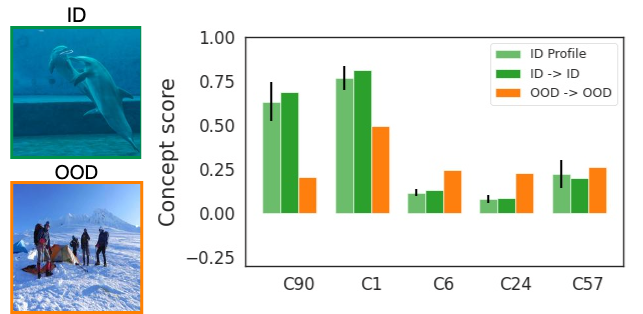
\includegraphics[width=\textwidth]{figures/figure1a.png}
         \caption{\small Correct detection: top dolphin image is correctly detected as ID (dark-green bar), and the bottom image is correctly detected as OOD (orange bar).}
         % ID (or OOD) dolphin image correctly detected as ID (or OOD).
         \label{fig:fig1a}
     \end{subfigure}
     \\
     \vspace{1mm}
     \begin{subfigure}[b]{\columnwidth}
         \centering
         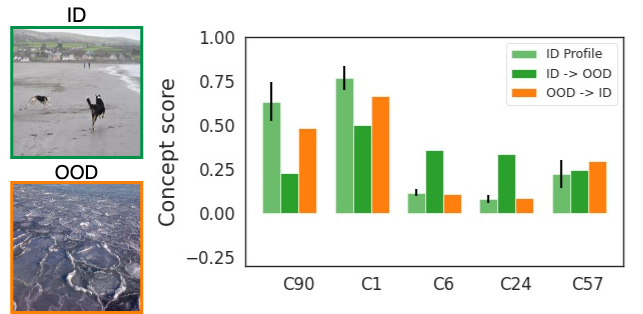
\includegraphics[width=\textwidth]{figures/figure1b.png}
         \caption{\small Wrong detection: top ID image is detected as OOD (dark-green bar), and the bottom OOD image is detected as ID (orange bar).}
         % ID (or OOD) dolphin image falsely detected as OOD (or ID).
         \label{fig:fig1b}
     \end{subfigure}
     \\
     \vspace{1mm}
     \begin{subfigure}[b]{\columnwidth}
         % \centering
         \hspace{1.5mm} 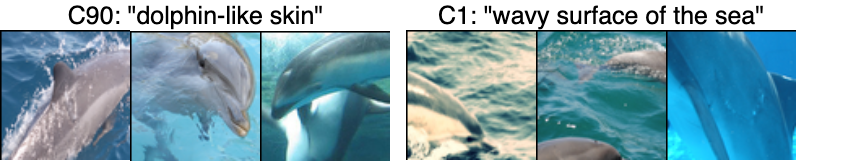
\includegraphics[width=\textwidth]{figures/dolphin_concepts.png}
         \caption{\small Visualization of top-2 important concepts.}
     \end{subfigure}
     \caption{\small \textbf{Our concept-based explanation for the Energy OOD detector~\citep{liu2020energy}.} All input images are classified as ``Dolphin'' but detected differently. On the x-axis of bar graphs, we present the top-5 important concepts that describe the detector's behavior given images classified as ``Dolphin''.
    % Both inputs are classified as "Zebra", but one is detected as ID and the other is detected as OOD by the detector.
    % Even though their class predictions are the same, an OOD-detected input may have very different concept patterns compared to that of an ID-detected input.
    ID profile (light-green) shows the average concept score pattern for ID images predicted as ``Dolphin''. We expect ID inputs predicted into this class to have a similar concept score pattern.}
\vspace{-5mm}
\label{fig:expl-ours-dolphin}
\end{figure}

This paper addresses the above research gap by proposing the first method (to our knowledge) for interpreting the decisions of an OOD detector in a human-understandable way.
We build upon recent advances in concept-based explanations for DNN classifiers~\citep{ghorbani2019ace,zhou2018interpretable,bouchacourt2019educe,yeh2020completeness}, which offer the benefit of providing explanations in terms of high-level {\em concepts} for classification tasks.
% \textcolor{blue}{Our method is unsupervised in that it does not require human-annotations for learning the concepts.}
We focus on extending this explanation framework to the problem of OOD detection.
% We make the first effort at extending their utility to the problem of OOD detection.
As a concrete example, consider Fig.~\ref{fig:expl-ours-dolphin} which illustrates our concept-based explanations given inputs which are all classified as the class ``Dolphin'' by a DNN classifier, but detected as either ID or OOD by an OOD detector.
Our method identifies that the concepts such as C90 ``dolphin-like skin'' and C1 ``wavy surface of the sea'' are key concepts to understand the OOD detector's decisions to tell apart ID and OOD images predicted as ``Dolphin''.
The user can verify that these concepts are aligned with human intuition and the OOD detector relies on them for making decisions.
We also confirm that the OOD detector predicts a certain input as ID when its concept-score patterns are similar to that of normal ID Dolphin images. Likewise, the detector predicts an input as OOD when its concept-score patterns are very different from that of ID inputs from the same class.
% A user can verify whether the OOD detector makes decisions based on the concepts that are aligned with human intuition (\eg ), and that the incorrect detection (as in Figure~\ref{fig:fig1b}) is an understandable mistake, not a misbehavior of the OOD detector.
Our explanations can help a user analyze if an incorrect detection (as in Fig.~\ref{fig:fig1b}) is an understandable mistake or a misbehavior of the OOD detector, evaluate the reliability of the OOD detector, and decide upon its adoption in practice.



% Unfortunately, being a statistical model, any OOD detector can make incorrect decisions, but we argue that it is important for an OOD detector to provide explanations when that occurs. 
% For instance, an OOD detector paired with a medical-diagnosis classifier may consistently detect a specific type of OOD input as ID, although the input may be clearly OOD to a human analyst. In such cases, it would be useful if the human analyst can extract an explanation for the detector's error to provide a better understanding of the detector's behavior.

% \textcolor{blue}{Aside from the }
% \jihye{@jayaram: I added the last sentence to give impression that explanations for OOD detector is helpful not only for misdetection but also for correct detections as well.}

% Recently, there has been an increasing number of works addressing the problem of learning 
% OOD detectors with better performance~\citep{liu2020energy,mohseni2020self,lin2021MOOD}.
% However, the problem of explaining the decisions of an OOD detector remains largely unexplored. Naturally, one may consider running an existing interpretation method for ML models (e.g., \citep{kim2018tcav, ghorbani2019ace}) on an example input, but that is inadequate in that it fails to provide insights as to why one example is ID while another is OOD.


% Extracting concept-based explanations, given any black-box OOD detector, is however challenging.
We aim to design a general interpretability framework that is applicable across a wide range of black-box OOD detectors.
Accordingly, a research question we ask is: {\em without relying on the internal mechanism of an OOD detector, can we identify a good set of concepts that are appropriate for understanding why the OOD detector predicts a certain input to be ID\,/\,OOD?} 
A key contribution of this paper is to show that this can be done unsupervised, without any additional human annotations for interpretation.
%
%with in-distribution and OOD data, respectively, and then inspecting the difference between the two generated explanations.
%Unfortunately, there is no guarantee that a method that can successfully explain a model's predictions can also be effective for OOD detectors.% Such mis-detections can hurt the human's trust in the detection algorithm, thus restricting the future use of the OOD detector in medical diagnosis.
% Having an algorithm that can explain the OOD detector's decisions might reveal that such mis-detected inputs were in-fact very similar to the in-distribution (ID) data.
%
%However, such misdetected OOD inputs could have been genuinely similar to in-distribution data, and those mistakes by the OOD detector would be negligible compared to its benefits. 
%Hence, understanding the behavior of OOD detectors is essential for their widespread adoption to real-world applications.
%
\iffalse

\begin{wrapfigure}{r}{0.5\linewidth}
\begin{center}
% \rule{0.9\linewidth}{0.75\linewidth}
% \begin{figure}[t]
% \vspace{1mm}
% 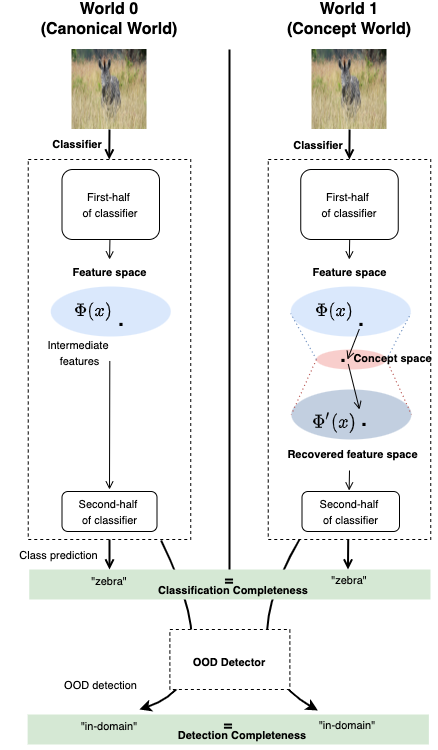
\includegraphics[width=0.45\textwidth]{figures/completeness.png}
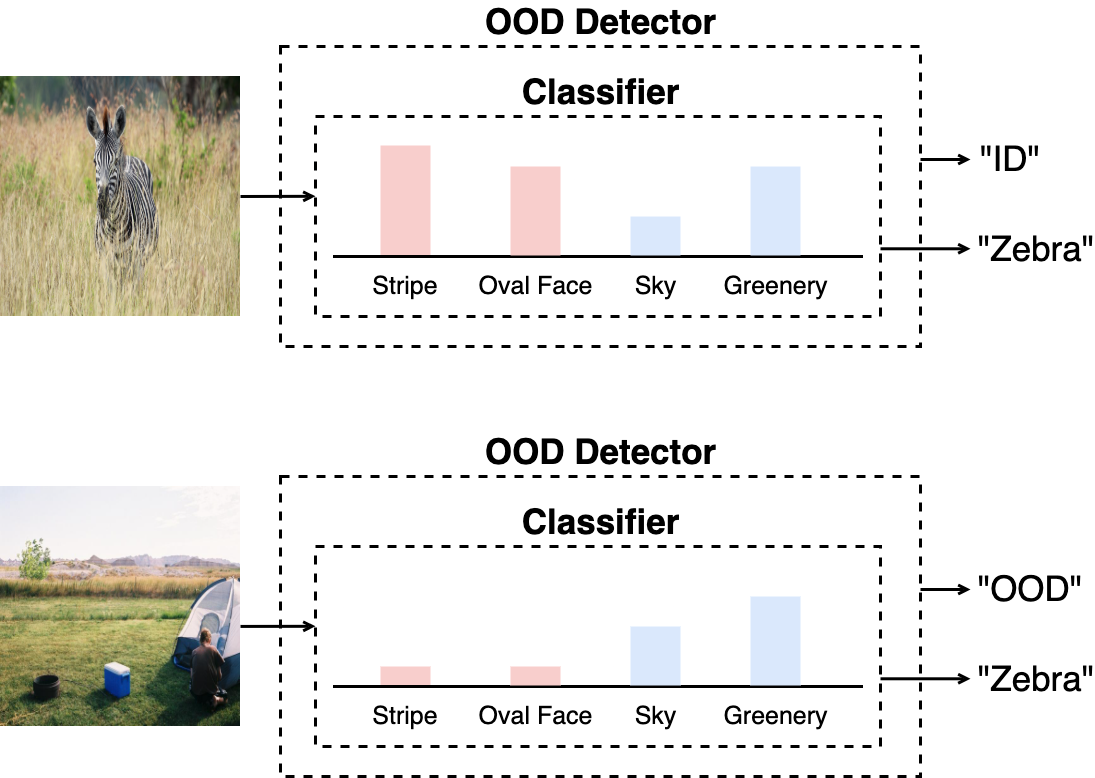
\includegraphics[scale=0.17]{figures/separability.png} 
\vspace{-3mm}
% \vspace{-0.1in}
\caption{\small \textbf{Our concept-based explanation for Energy detector~\citep{liu2020energy}.} "Stripe", "Oval Face", "Sky" and "Greenery" are concepts that completely explain the behavior of the classifier and OOD detector.
% Both inputs are classified as "Zebra", but one is detected as ID and the other is detected as OOD by the detector.
Even though their class predictions are the same, an OOD-detected input may have very different concept patterns compared to that of an ID-detected input.}
% \vspace{-8mm}
\label{fig:detection-separability}
\end{center}
\vspace{-0.12in}
% \end{figure}
\end{wrapfigure}

\begin{figure}[t]
\centering
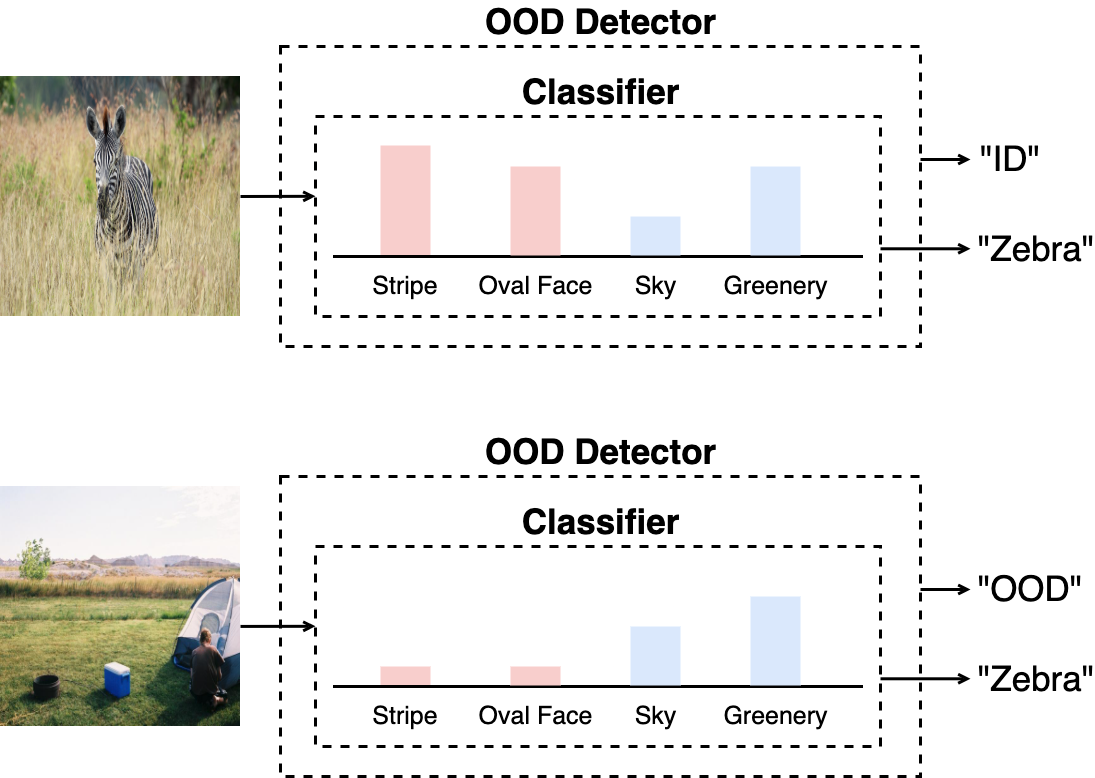
\includegraphics[scale=0.17]{figures/separability.png} 
\caption{ \textbf{Concept-based explanation for OOD detector.} "Stripe", "Oval Face", "Sky" and "Greenery" are concepts that completely explain the behavior of the classifier and OOD detector.
% Both inputs are classified as "Zebra", but one is detected as ID and the other is detected as OOD by the detector.
Even though their class predictions are the same, an OOD-detected input may have very different concept patterns compared to that of an ID-detected input.}
\label{fig:detection-separability}
\end{figure}

\fi
%

In summary, we make the following contributions:
\begin{itemize} [leftmargin=*, topsep=1pt, noitemsep]
% \begin{itemize}
\item We motivate and propose new metrics to quantify the effectiveness of concept-based explanations for a black-box OOD detector, namely \textit{detection completeness} and \textit{concept separability} (Sections \ref{sec:two_worlds}, \ref{sec:completeness_score}, and \ref{sec:separability_score}).  
\item We propose a concept-learning objective with suitable regularization terms that, given an OOD detector for a DNN classifier, learns a set of concepts with high detection completeness and concept separability (Section~\ref{sec:concept_learning});
% \item We introduce regularization terms and propose a method, which given an OOD detector for a DNN classifier, learns a set of concepts that have good detection completeness and concept separability (\S~\ref{sec:concept_learning});
% \item Our empirical results with popular OOD-detectors confirm the insight that concepts with high values for the proposed metrics provide a much clearer distinction for explaining detected-ID and detected-OOD inputs.
\item By treating the OOD detector as a black-box, we show that our approach can be applied to explain a variety of existing OOD detection methods.
% We evaluate the proposed concept learning on popular OOD detectors with multiple real-world datasets. 
We also provide empirical evidence that concepts learned for classifiers cannot be directly used to explain OOD detectors, whereas concepts learned by our method are effective for explaining both the classifier and OOD detector (Section~\ref{sec:eval-concept}).
% which supports the need for our concept discovery method and proposed metrics.
\item By identifying prominent concepts that contribute to an OOD detector's decisions via a modified Shapley value importance score based on the detection completeness, we demonstrate how the discovered concepts can be used to interpret the OOD detector (Section~\ref{sec:expt_concept_based_explanations}).
\end{itemize}


\mypara{Related Work. }  In the literature of OOD detection, recent studies have designed various scoring functions based on the representation from the final or penultimate layers \citep{liang2018ODIN, devries2018learning}, or a combination of different internal layers of a DNN classifier~\citep{lee2018mahalanobis, lin2021MOOD, raghuram2021JTLA}.
A recent survey on generalized OOD detection can be found in Yang et al.~\citep{yang2021survey}. Our work aims to provide post-hoc explanations applicable to a wide range of black-box OOD detectors without modifying their internals.
Among different interpretability approaches, concept-based explanation~\citep{koh2020concept-bottleneck, SENN} has gained popularity as it is designed to be better-aligned with human reasoning \citep{armstrong1983human-concepts,tenenbaum1999concept-learning} and intuition~\citep{ghorbani2019ace,zhou2018interpretable,bouchacourt2019educe,yeh2020completeness}. There have been limited attempts to assess the use of concept-based explanations under data distribution changes such as adversarial manipulation~\citep{kim2018tcav} or spurious correlations~\citep{adebayo2020debugging}.
However, designing concept-based explanations for OOD detection requires further exploration and is the focus of our work.
% Feature attribution is the most commonly used post-hoc explanation method that attributes the decision to local input features~\citep{baehrens2009grad, simonyan2013grad, smilkov2017smoothgrad, sundararajan2017IG}, but recent works have demonstrated its vulnerability to \eg adversarial perturbations~\citep{ghorbani2019fragile,heo2019fooling,slack2020fooling}. 
% \citept{adebayo2020debugging} also conduct experimental analyses and a human subject study to assess the effectiveness of feature attributions under various settings (including on OOD data), and show that feature attributions barely have any visual difference between ID inputs and OOD inputs.
%To the best of our knowledge, we are the first to study concept-based interpretability for explaining the behavior of OOD detectors.
% \textcolor{blue}{Add a pointer to a more detailed related work section in the appendix.}



\iffalse

Once machine learning (ML) model is deployed in real-world settings, it often encounters inadvertent situations.
Specifically, with OOD inputs, drawn from an unknown distribution that the model has not been exposed to during training, it can yield uncertain and unreliable decisions \citep{amodei2016AISafety,goodfellow2015explaining,nguyen2015posterior}.
The most common practice to avoid such phenomenon is to associate a detector that identifies whether an incoming input is likely to be OOD, then reject the model's decision on the OOD input \citep{hendrycks2018OE,lin2021MOOD,mohseni2020self}.
While a plethora of works have focused on bringing better-performing algorithmic approaches for OOD detection, however, there is little effort to reason about their decisions.
Limited understanding of OOD detection results can confine the adoption of the OOD detection methods: for instance, an OOD detector paired with a medical diagnosis model may consistently detect a specific type of OOD data as in-distribution, while those data genuinely share common attributes with in-distribution data.
Even when such misdetection could be reasonably understandable to humans, it could restrict the future use of OOD detection methods in medical diagnosis.
% Hence, it is critical to interpret existing OOD detectors in a human-understandable way.
To this end, we aim to develop an effective method targeted to OOD detector explanations.
% Not limited to simply avoiding misleading behaviors of models, however, to develop better-performing and more reliable models, we need to understand \jihye{reliability of ood detector and its decision.}
% Suppose ...., then a ML practitioner can decide .... to ...(improve) the model \jihye{simple use case of our method}

A natural approach to explain OOD detectors would be running an existing interpretation method with in-distribution and OOD data, respectively, and then inspecting the difference between the two generated explanations \citep{}.
Unfortunately, there is no guarantee that the method that could successfully explain model predictions can also be effective for the use case.
For instance, feature attribution is the most commonly used type of explanation, but it is known to be unreliable even to invisible manipulation of inputs \citep{}
\citep{adebayo2020debugging} study the effectiveness of feature attributions specifically with OOD data through human subject tests and experimental analysis; they show that feature attributions make no visual difference between ID inputs and OOD inputs, and therefore, might not be intuitive guidance for humans when deciding whether to trust model predictions with OOD inputs. 
Other than feature attributions, concept-based explanation is another line of model explanation methods with the advantage of using human-friendly, high-level concepts, but related works have only focused on their usage for understanding model predictions \citep{}.

\jihye{Below are incomplete}

Notwithstanding the rapid growth of ML explainability and the development of high-performance OOD detector, little work has been done to reason about OOD detection.
This paper takes a step toward interpreting what makes data to be detected as in-distribution or OOD, and what are the distinguishing characteristics between in-distribution and OOD data.
% A natural approach would be running an existing explanation method with in-distribution and OOD data, and inspecting the difference between the generated explanations of in-distribution and OOD.
% Unfortunately, one caveat with \jihye{...} is that the method would provide reliable and intuitive explanation with in-distribution inputs, but are not guaranteed to covey reliable, and easy-to-interpret information to reason about the model's behavior given OOD inputs.
% For instance, feature attribution methods \citep{baehrens2009grad, simonyan2013grad, smilkov2017smoothgrad, sundararajan2017IG} that successfully assess relevance of the dimensions of in-distribution input to a model’s output, fail to capture visual distinguishability between in-distribution attribution and OOD attribution \citep{adebayo2020debugging}.
% Moreover, \citep{adebayo2020debugging} shows that explanation by the presentation of visually similar attributions may not be an informative guide for human users to decide the trustworthiness of model decision.
For instance, feature attributions are the most popular local explanation method \citep{baehrens2009grad, simonyan2013grad, smilkov2017smoothgrad, sundararajan2017IG}, but they fail to assist human users' decision on the reliability of model outputs, due to no visual difference between in-distribution and OOD attributions \citep{adebayo2020debugging}. 
Moreover, they are limited to discovering the 

Better aligned with human concept-based thinking \jihye{cite Tenenbaum, Armstrong}, ...
Concept-based explanation characterizes the global behavior of model in terms of intuitive, human-understandable concepts \citep{kim2018tcav, ghorbani2019ace, yeh2020completeness}, but their \textit{appropriateness} for OOD detection tasks are not investigated yet.
We propose to extend their usage to OOD detection, and evaluate the effectiveness/appropriateness? -- in terms of detection completeness and separability.
\jihye{intuition and brief description of detection completeness and separability}.
\jihye{clarification on the meaning of providing explanations for ood detection. It is not our goal to understand the model coverage on ID samples in terms of concepts}
We also extend \citep{yeh2020completeness}'s unsupervised approach to concept discovery to learn a set of concepts with high detection completeness and separability scores.\\
% Motivated by the intuitiveness \jihye{human-understandable? user-friendly?} of concept-based explainability, we aim to extend the use of high-level concepts into OOD detection.
% In this paper, (our goal)
% \jihye{find a set of concepts that are not just completely describing the behavior of DNN classifier, } 
% However, as demonstrated in Section \jihye{()},

WIth the set of concepts, describe what kind of explanations we provide.... \\.\\.\\.\\.\\.\\.\\.

Our contributions can be summarized as follows:
\begin{itemize}[leftmargin=*, topsep=1pt, noitemsep]
    \item Our work is the first quantitative and qualitative evaluation on the appropriateness of high-level concepts toward OOD detection explanation.
    We introduce two metrics for the quantitative evaluation of concepts -- detection completeness and separability.
    \item We propose an unsupervised \jihye{by saying unsupervised, I mean we don't involve extra annotations for concepts} learning framework to find concepts that possess the desired properties.
    \jihye{also, theoretical analysis on how separability in concept scores is related to the separability in OOD scores?}
    \item We verify the effectiveness of our framework to extract concepts for real-world image datasets and popular OOD detectors, and demonstrate insights into the behavior of OOD detectors.
\end{itemize}

\fi

\section{Problem Setup and Background}
\mypara{Notations.}
Let $\inputs \subseteq \reals^{a_0 \times b_0 \times d_0}$ denote the space of inputs $\bfx$, where $d_0$ is the number of channels and $a_0$ and $b_0$ are the image size along each channel.
Let $\outputs := \{1, \cdots, L\}$ denote the space of output class labels $y$.
Let $\simplex_L$ denote the set of all probabilities over $\outputs$ (the simplex in $L$-dimensions).
We assume that natural inputs to the DNN classifier are sampled from an unknown probability distribution $\Pin$ over the space $\calX \times \outputs$.  
The  compact notation $[n]$ denotes $\{1, \cdots, n\}$ for a positive integer $n$.
Boldface symbols are used to denote both vectors and tensors.
$\langle\bfx, \bfx^\prime\rangle$ denotes the standard inner-product between a pair of vectors. 
% In the case of vectors, it is the standard $\bfx^T \,\bfx$. 
% In the case of image tensors $\bfx, \,\bfx^\prime \in \reals^{a \times b \times c}$, the inner-product is defined as the vector product along the third dimension. That is $\,\bfz = \langle\bfx, \bfx^\prime\rangle \in \reals^{a \times b}$ with $\,z_{ij} = \sum_{k=1}^c x_{ijk} \,x^\prime_{ijk}, ~i \in [a], j \in [b]$.
The indicator function $\indicator[c]$ takes value $1$ ($0$) when the condition $c$ is true (false).

\mypara{ID and OOD Datasets.}
% Throughout the paper, 
Consider a labeled ID training dataset $\Dintr = \{(\bfx_i, y_i), ~i = 1, \cdots, \Nintr\}$ sampled from the distribution $\Pin$.
We assume the availability of an unlabeled training dataset $\Douttr = \{\widetilde{\bfx}_i, ~i = 1, \cdots, \Nouttr\}$ from a different distribution, referred to as the {\em auxiliary OOD dataset}.
Similarly, we define the ID test dataset (from $\Pin$) as $\Dinte$, and the OOD test dataset as $\Doutte$.
Note that the auxiliary OOD dataset $\Dintr$ and the test OOD dataset $\Doutte$ are from different distributions.
All the OOD datasets are unlabeled since their label space is usually different from $\outputs$. 
% One can think of the OOD datasets for training, validation, and test to be biased samples from an unknown OOD marginal distribution $\Pout(\bfx)$.

\mypara{OOD Detector.}
%\label{sec:ood_detector}
The goal of an OOD detector is to determine if a test input to the classifier is ID (\ie from the distribution $\Pin$); otherwise the input is declared to be OOD~\citep{yang2021survey}.
Given a trained classifier $\bff : \calX \mapsto \Delta_L$, the decision function of an OOD detector can be generally defined as $\,\calD_\gamma(\bfx, \bff) \,=\, \indicator[S(\bfx, \bff) \geq \gamma]$, where $S(\bfx, \bff) \in \reals$ is the score function of the detector for an input $\bfx$ and $\gamma$ is the threshold.
%
\iffalse

Given a trained classifier $\bff$, the decision function of an OOD detector can be generally defined as~\citep{liu2020energy},
% \vspace{-3mm}
\begin{equation}
\label{eq:ood_detector}
\calD_\gamma(\bfx, \bff) ~=~ 
\begin{cases}
1, & \text{if } ~S(\bfx, \bff) \geq \gamma \\
0, & \text{otherwise }
\end{cases}
\end{equation}
where $S(\bfx, \bff) \in \reals$ is the score function of the detector for an input $\bfx \in \calX$, and $\gamma$ is the threshold.

\fi
%
We follow the convention that larger scores correspond to ID inputs, and the detector outputs of $1$ and $0$ correspond to ID and OOD respectively.
% For the brevity of notation, we use $\calD_\gamma(\bfx, \bff)$ and $\calD_\gamma$ interchangeably.
% Common choices for $S(\bfx, \bff)$ include the softmax confidence score (\ie the maximum predicted probability)~\citep{hendrycks2016msp}, the Energy score computed from logits at the penultimate layer~\citep{liu2020energy}, the negative maximum of the unnormalized logits~\citep{hendrycks2019scaling}, and other combined statistics from the intermediate feature representations~\citep{lee2018mahalanobis,raghuram2021JTLA}.
%It is worth noting that most of these methods for OOD detection can be modified to predict using the feature representation reconstructed from the concept space (\ie using $\recphi(\bfx)$). 
We assume the availability a pre-trained DNN classifier and a paired OOD detector that is 
trained to detect inputs for the classifier.

% \vspace{-0.1in}
\subsection{Projection Into Concept Space}
\label{sec:concept_projection}

% \begin{wrapfigure}{r}{0.5\linewidth}
\begin{figure}[ht]
\centering
% \rule{0.9\linewidth}{0.75\linewidth}
% \begin{figure}[t]
% \vspace{-0.2in}
% 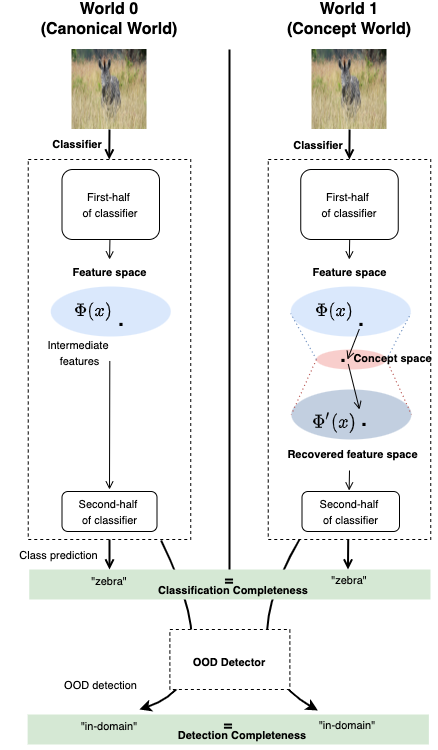
\includegraphics[width=0.45\textwidth]{figures/completeness.png}
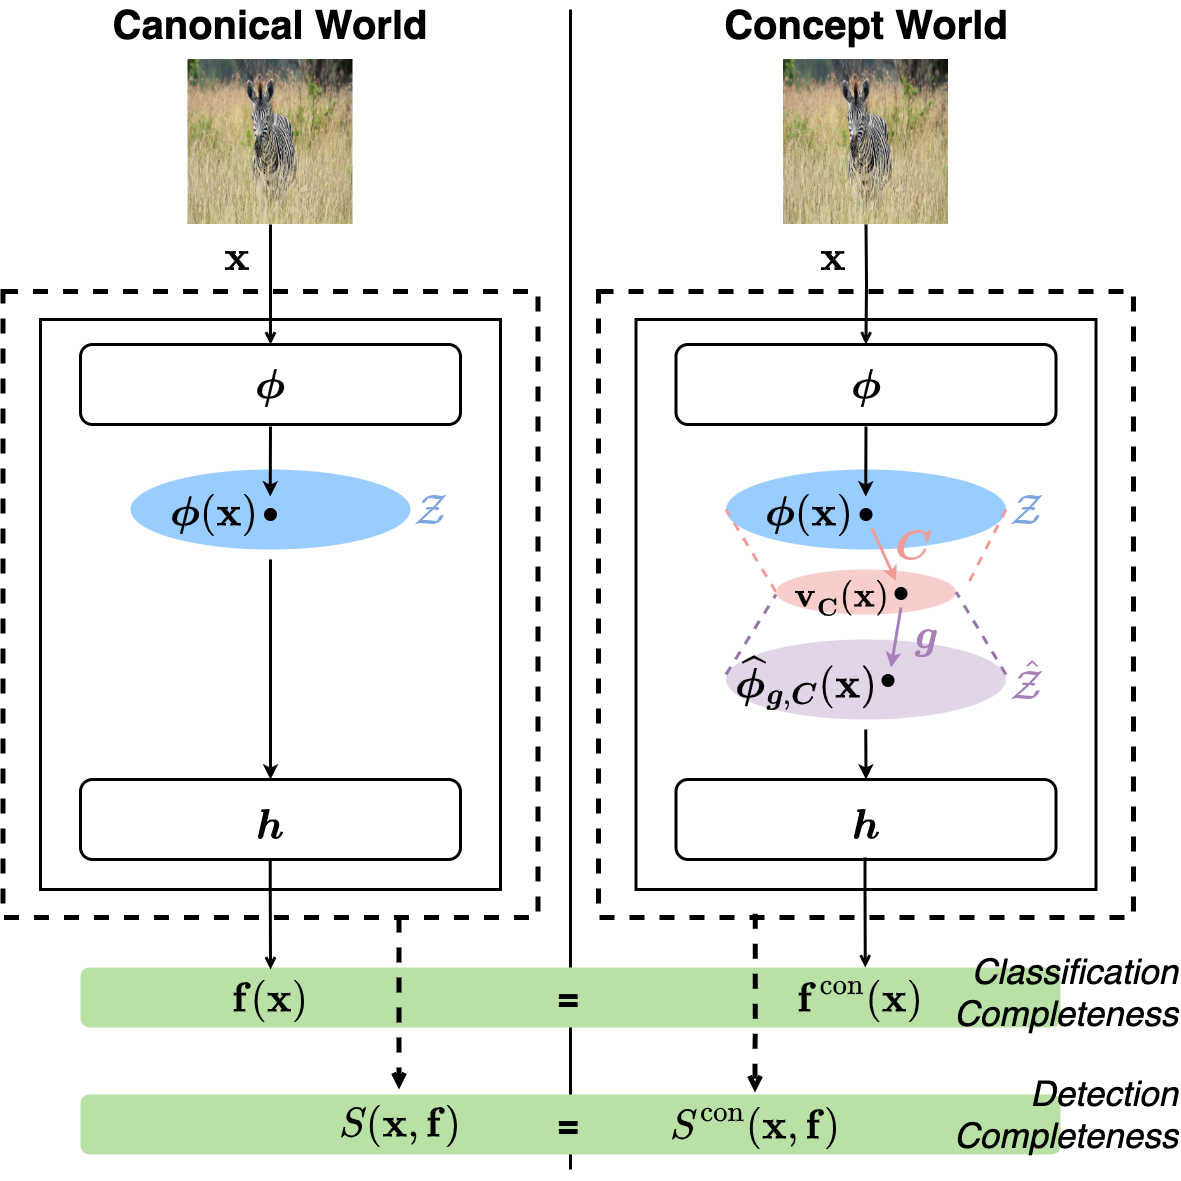
\includegraphics[scale=0.17]{figures/completeness_3.png} 
%\vspace{-2mm}
% \vspace{-0.2in}
\caption{
\textbf{Our two-world view of the classifier and OOD detector.} In the canonical world, both the classifier and OOD detector are unmodified. In the concept world, the layer representation $\bfphi(\bfx)$ is projected into the space spanned by the concept vectors and then reconstructed via the non-linear mapping $\bfg$. The classifier and OOD detector in the concept world are based on this reconstructed layer representation. Given the same input, the outputs from the DNN classifier and OOD detector in both the worlds should be very close to each other (characterized by \textit{Classification Completeness} and \textit{Detection Completeness}, respectively).
}
% \vspace{-3mm}
\label{fig:detection-completeness}
\vspace{-0.19in}
\end{figure}
% \end{wrapfigure}
%
\iffalse

\caption{\small \textbf{Our two-world view of the classifier and OOD detector.} Ideally, given the same input, the outputs both from the DNN classifier and OOD detector should be identical between the two worlds (characterized by \textit{Classification Completeness} and \textit{Detection Completeness}, respectively.)}

\begin{figure}[t]
\centering
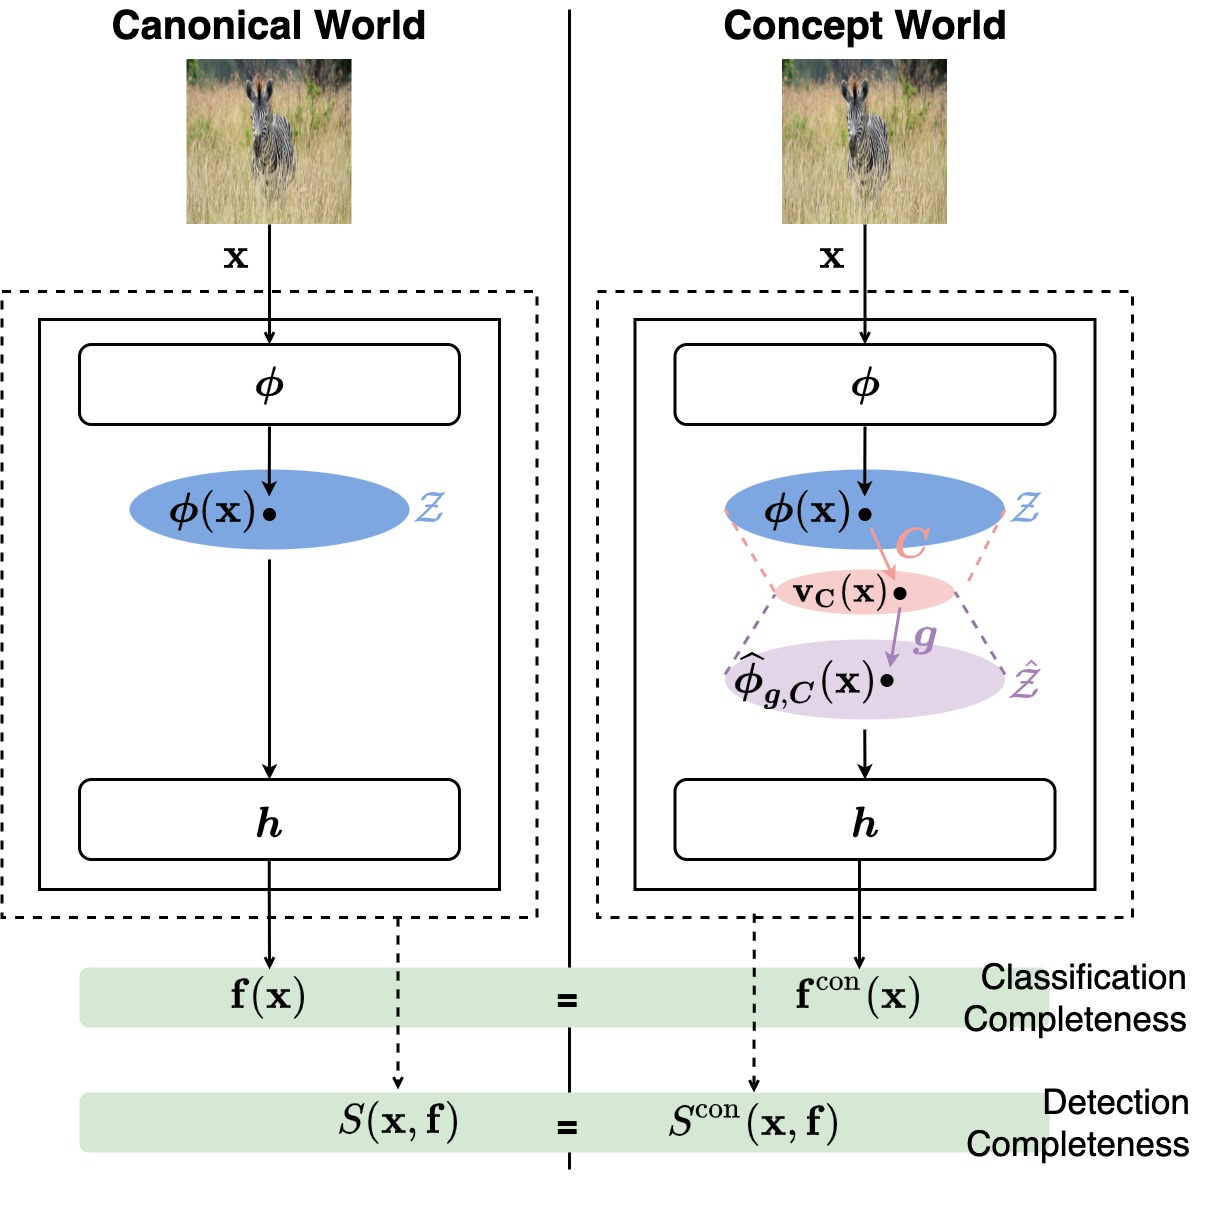
\includegraphics[scale=0.17]{figures/completeness_3.jpeg} 
\caption{\textbf{Our two-world view of the classifier and OOD detector.}}
\label{fig:detection-completeness}
\end{figure}

\fi

Consider a pre-trained DNN classifier $\bff : \mathcal{X} \mapsto \simplex_L$ that maps an input $\bfx$ to its corresponding predicted class probabilities. 
Without loss of generality, we can partition the DNN at a convolutional layer $\ell$ into two parts, \ie $\bff = \bfh \circ \bfphi$ where: 1) $\bfphi : \inputs \mapsto \calZ := \reals^{a_\ell b_\ell \times d_\ell}\,$ is the first half of $\bff$ that maps an input $\bfx$ to the intermediate feature representation~\footnote{We flatten the first two dimensions of the feature representation, thus changing an $a_\ell \times b_\ell \times d_\ell$ tensor to an $a_\ell b_\ell \times d_\ell$ matrix, where $a_\ell$ and $b_\ell$ are the filter size and $d_\ell$ is the number of channels.} $\bfphi(\bfx)$, and 2) $\bfh : \calZ \mapsto \simplex_L$ is the second half of $\bff$ that maps $\bfphi(\bfx)$ to the predicted class probabilities $\bfh(\bfphi(\bfx))$.
% For the feature representation at layer $\ell$, $d_\ell$ is the number of channels and $a_\ell$ and $b_\ell$ are the filter size (\eg $d_\ell = 2048$, $a_\ell = b_\ell = 5$ at the layer right before the global-pooling layer of the Inception-v3 network~\citep{szegedy2016inception-v3}).
We denote the predicted probability of a class $y$ by $\,f_y(\bfx) = h_y(\bfphi(\bfx))$, and the prediction of the classifier by $\,\widehat{y}(\bfx) = \argmax_{y} f_y(\bfx)$.

% \ap{I  brought in some stuff from Concept  Scores para in Section 3 to the following para to avoid duplication and ensure consistency. But, more I read it, I think the entire para on Concept Scores from there should be merged here. It is not clear by the way whether concept scores is from prior art or we are introducing it. No cites are given.}

Our work is based on the common implicit assumption of linear interpretability in the concept-based explanation literature, \ie high-level concepts lie in a linearly-projected subspace of the feature representation space $\calZ$ of the classifier~\citep{kim2018tcav}. 
% We explore the setting where high-level concepts lie in a subspace of the feature-representation space $\calZ$ of the classifier. 
% The feature representation is typically high-dimensional, \eg at the layer right before the global-pooling layer of the Inception-V3 network~\citep{szegedy2016inception-v3}, the dimension would be $25 \times 2048$ ($d_\ell = 2048, \,a_\ell = b_\ell = 5$).
Consider a projection matrix $\,\bfC = [\bfc_1, \cdots, \bfc_m] \in \reals^{d_\ell \times m}$ (with $m \ll d_\ell$) that maps from the space $\calZ$ into a reduced-dimension concept space. 
$\bfC$ consists of $m$ unit vectors, where $\bfc_i \in \reals^{d_\ell}$ is referred to as the \textit{concept vector} representing the $i$-th concept (\eg ``stripe'' or ``oval face''), and $m$ is the number of concepts.
% Based on the assumption that high-level concepts lie in a subspace of a feature-representation space of the classifier, consider a projection $\bfC \in \reals^{d_\ell \times m}$ (with $m \ll d_\ell$) that maps from the feature space into a reduced-dimension concept space (\eg a striped pattern). 
% \ryan{could be worth expanding on what the concepts could be since "stripe" can be ambiguous if the reviewers fail to connect it with figure 1}.
% We define the linear projection of a high-dimensional layer representation $\bfphi(\bfx) \in \reals^{a_\ell b_\ell \times d_\ell}$ into the concept space by $\,\VC(\bfx) := \bfphi(\bfx)\, \bfC \,\in \reals^{a_\ell b_\ell \times m}$. 
We define the \textit{concept score} for $\bfx$ as the linear projection of the high-dimensional layer representation $\bfphi(\bfx) \in \reals^{a_\ell b_\ell \times d_\ell}$ into the concept space~\citep{yeh2020completeness}, i.e. $\,\VC(\bfx) := \bfphi(\bfx)\, \bfC \,\in \reals^{a_\ell b_\ell \times m}$.
% This is referred to as the \textit{concept score} for $\bfx$ corresponding to the projection matrix $\bfC$~\citep{yeh2020completeness}.
% \ap{Is this our definition of concept score? Else we should cite prior art.}
% That is, $\bfv_{\bfC}(\bfx) := \bfC \bfphi(\bfx)$ is the \textit{concept score} for $\bfx$ defined by the projection matrix $\bfC$.
We also define a mapping from the projected concept space back to the feature space by a non-linear function $\,\bfg : \reals^{a_\ell b_\ell \times m} \mapsto \reals^{a_\ell b_\ell \times d_\ell}$.
% We define this reconstruction of the feature representation at layer $\ell$ from the concept space by $\,\recphi(\bfx) \,:=\, \bfg(\VC(\bfx))$.
The reconstructed feature representation at layer $\ell$ is then defined as $\,\recphi(\bfx) \,:=\, \bfg(\VC(\bfx))$.
% We note that $\bfg$ could be non-linear.
% To be precise, let $\,\recphi(\bfx) = \bfg(\VC(\bfx))$ define the reconstructed feature representation.
%Note that any DNN classifier can be modified to make predictions based on the reconstructed feature representation instead of the original feature representation.


% \vspace{-.1in}
\subsection{Canonical World and Concept World}
\label{sec:two_worlds}
% \mypara{Canonical World and Concept World.}
As shown in Fig.~\ref{fig:detection-completeness}, we consider a ``two-world'' view of the classifier and OOD detector consisting of the {\em canonical world} and the {\em concept world}, which are defined as follows:

\mypara{Canonical World.}
In this case, both the classifier and OOD detector use the original layer representation $\bfphi(\bfx)$ for their predictions. The prediction of the classifier is $\,\bff(\bfx) = \bfh(\bfphi(\bfx))$, and the decision function of the detector is $\,\calD_\gamma(\bfx, \bfh \circ \bfphi)$ with a score function $S(\bfx, \bfh \circ \bfphi)$.

% \mypara{\textbf{World 1 (\textit{concept world}).}}
\mypara{Concept World.}
% In this world, both the class prediction and OOD detection are based on the reconstructed feature representation $\recphi(\bfx)$ as shown in the right half of Fig.~\ref{fig:detection-completeness}.
We use the following observation in constructing the concept-world formulation: {\em both the classifier and the OOD detector can be modified to make predictions based on the reconstructed feature representation}, \ie using $\recphi(\bfx)$ instead of $\bfphi(\bfx)$. 
% This idea is illustrated in the right half of Fig.~\ref{fig:detection-completeness}. 
Accordingly, we define the corresponding classifier, detector, and score function in the concept world as follows:
\begin{align}
\label{equ:concept_world}
\centering
\fcon(\bfx) ~&:=~ \bfh(\recphi(\bfx)) ~=~ \bfh(\bfg(\VC(\bfx))) \nonumber \\
\Dcon(\bfx, \bff) \,&:=\, \calD_\gamma(\bfx, \bfh \circ \recphi) \,=\, \calD_\gamma(\bfx, \bfh \circ \bfg \circ \VC) \nonumber \\
\centering
\Scon(\bfx, \bff) \,&:=\, S(\bfx, \bfh \circ \recphi) \,=\, S(\bfx, \bfh \circ \bfg \circ \VC).
\end{align}
%
%1) {\em canonical world}, where both the classifier and detector use the original layer representation $\bfphi(\bfx)$ for their predictions; 
%2) {\em concept world}, where both the classifier and detector use the concept score-based reconstruction of the layer representation $\recphi(\bfx)$ for their predictions. 
%
We further elaborate on this two-world view and introduce the following two desirable properties.
% , viz. detection completeness and concept separability.

% Such observation gives rise to two worlds where a DNN classifier and an OOD detector can be in (outlined in Figure \ref{fig:detection-completeness}):
% % This is the starting point of our work.
% \jihye{formatting the following two paragraphs: indent/list?}

% \mypara{\textbf{World 0 (\textit{canonical world}).}} 

%
\mypara{Detection Completeness.} Given a fixed algorithmic approach for learning the classifier and OOD detector, and with fixed internal parameters of $\bff$, we would ideally like the classifier prediction and the detection score to be indistinguishable between the two worlds. 
In other words, for the concepts to \textit{sufficiently} explain the OOD detector, we require $\Dcon(\bfx, \bff)$ to closely mimic $\calD_\gamma(\bfx, \bff)$. 
Likewise, we require $\fcon(\bfx)$ to closely mimic $\bff(\bfx)$ since the detection mechanism of $\calD_\gamma$ is closely paired to the classifier.
We refer to this property as the {\em completeness of a set of concepts with respect to the OOD detector and its paired classifier.}  
% As discussed in \S~\ref{sec:completeness_score}, this extends the notion of classification completeness introduced by~\citet{yeh2020completeness} for a classifier to a pair consisting of both the OOD detector along with its paired classifier.
As discussed in \S~\ref{sec:completeness_score}, this extends the notion of classification completeness introduced by~\citet{yeh2020completeness} to an OOD detector and its paired classifier.
% This translates to finding an optimal set of concept vectors $\bfC$ and a reconstruction network $\bfg$ to achieve the above goals.


\iffalse

We assume that with a fixed algorithmic approach for $\calD$ and a fixed internals of $\bff$, the classifier output and detection score should be indistinguishable between the two worlds.
In other words, for concepts to \textit{sufficiently} explain an OOD detector, $\Dcon(\bfx, \bff)$ should mimic $\calD_\gamma(\bfx, \bff)$ sufficiently well. 
Likewise, we require $\fcon(\bfx)$ to imitate $\bff(\bfx)$ sufficiently well, as the algorithm of $\calD$ is paired with $\bff$.
If the performance gap between the two worlds is large, one should not trust that the explanations resulted from $\bfC$ are accurate description of the target detector $\calD$.

To improve the interpretability of the resulting explanations, we impose another important property on the learned concepts: data detected as ID by $\calD_\gamma$ (henceforth referred to as \textit{ID-detected} data) and data detected as OOD by $\calD_\gamma$ (henceforth referred to as \textit{OOD-detected} data) should be well separated in the concept space.
Refer to Figure \ref{fig:detection-separability} for illustration purposes.
While the ID input and OOD input show clear distinctive patterns for concept "Stripe" and "Oval Face", concept "Sky" and "Greenery" would decrease the overall distinction between the two inputs in terms of concepts. 
The four concepts might be sufficient to close the gap between canonical world and concept world, but considering that our work aims to guide humans to understand what concepts distinguish ID data and OOD data, we would prefer a set of concepts that have well-separated pattern for different detection outputs.

\fi

\mypara{Concept Separability.} To improve the interpretability of the resulting explanations for the OOD detector, we require another desirable property from the learned concepts: data detected as ID by $\calD_\gamma$ (henceforth referred to as \textit{detected-ID} data) and data detected as OOD by $\calD_\gamma$ (henceforth referred to as \textit{detected-OOD} data) should be well-separated in the concept-score space.
Since our goal is to help an analyst understand which concepts distinguish the detected-ID data from detected-OOD data, we would like to learn a set of concepts that have a well-separated concept score pattern for inputs from these two groups (\eg the concepts $C_{90}$ and $C_1$ in Fig.~\ref{fig:expl-ours-dolphin} have distinct concept scores).
% Going back to Fig.~\ref{fig:detection-separability} for illustration, 
% While the concepts ``stripe'' and ``oval face'' show clear distinctive patterns between the inputs, concepts ``sky'' and ``greenery'' have a similar concept-score pattern. 
% , even when their class predictions are identical.
% for different detection outputs.

%Include the following para if space permits.
%In summary, we identify two desirable properties for the learned concepts in order to explain the OOD detector sufficiently well: (1) Detection completeness: the concept scores are essentially sufficient statistics for recovering the performance of the OOD detector and its paired classifier in the concept world; and (2)  Concept separability: for improved interpretability of the detector, the detected-ID data and detected-OOD data should have clearly-distinctive patterns in the concept world. 
% We next propose a method for learning such concepts.

\iffalse

In summary, we identify two desirable properties for the learned concepts in order to explain the OOD detector sufficiently well: (1) Detection completeness:  The concept scores are essentially sufficient statistics for recovering the performance of the OOD detector (\eg area under the ROC curve) and its paired classifier (\eg accuracy) in the concept world; and (2)  Concept separability: For improved interpretability of the detector, the detected-ID data and detected-OOD data should have clearly-distinctive patterns in the concept world. We next propose a method for learning such concepts.
% \jihye{using detector as oracle.}

\fi





\vspace{-.05in}
\section{Proposed Approach}
Given a trained DNN classifier $\bff$, a paired OOD detector $\calD_\gamma$, and a set of concepts $\bfC$, we address the following questions: \textbf{1)} \emph{Are the concepts sufficient to capture the prediction behavior of both the classifier and OOD detector?} (see \S~\ref{sec:completeness_score}); \textbf{2)} \emph{Do the concepts show clear distinctions in their scores between detected-ID data and detected-OOD data?} (see \S~\ref{sec:separability_score}). 
We first propose new metrics for quantifying the set of learned concepts, followed by a general framework for learning concepts that possess these properties (see \S~\ref{sec:concept_learning}).
% We propose a general framework for learning a set of concepts that possess these properties (\S~\ref{sec:concept_learning}).
% This section explains our evaluation metrics and methods: (1) how to gauge the utility of a given set of concepts for OOD detector explanation, and (2) a general learning algorithm to discover concepts that \jihye{incomplete yet}

\subsection{Metric for Detection Completeness}
\label{sec:completeness_score}
% To address the question of whether a set of learned concepts are sufficient to capture the behavior of the classifier and OOD detector, we next define completeness scores with respect to the classification task and the detection task. 
%
% We address the following questions: 1) \textit{are the set of concepts sufficient to similarly match the behavior of the original classifier $\bff$}, and 2) \textit{are the set of concepts sufficient to similarly match the behavior of the OOD detector $\calD_\gamma$?} 
% Such properties would indicate that the concepts are appropriate for describing the behavior of $\bfC$ and $\calD_\gamma$.
%
% Given a trained DNN classifier $\bff$ and a trained OOD detector $\calD_\gamma$, our goal is to learn a set of concepts that can provide explanations for the predictions of the classifier and detector.
% To this end, we first propose new metrics for quantifying a set of learned concepts, followed by a general framework for learning a set of concepts.
% Given a sufficient set of concepts $\bfC$, the classifier in the concept world should be able to closely approximate the prediction performance of the original classifier.
% Likewise, the detector in the concept world should be able to closely approximate the detection performance of the original detector.
% In order to concretely quantify these properties, we hereby define a 
% completeness score for the set of concepts with respect to the classification task and the OOD detection task.
%
\begin{definition}
\label{def:completeness_class}
Given a trained DNN classifier $\bff = \bfh \circ \bfphi\,$ and a set of concept vectors $\bfC$, the {\em classification completeness} with respect to $\Pin(\bfx, y)$ is defined as \citep{yeh2020completeness}:
\begin{align*}
% \label{equ: completeness-classification}
    &\eta^{}_\bff(\bfC) := \\
    &\frac{\textrm{sup}_\bfg \,\expec_{(\bfx, y) \sim \Pin} \!\big[ \indicator[ y = \argmax_{y'} h_{y'}(\recphi(\bfx)) ] \big] ~-~ a_r}{\expec_{(\bfx, y) \sim \Pin} \!\big[ \indicator[y = \argmax_{y'} h_{y'}(\bfphi(\bfx))] \big] ~-~ a_r}
\end{align*}
where $a_r = 1 / L$ is the accuracy of a random classifier.
\end{definition}
The denominator of $\eta^{}_\bff(\bfC)$ is the accuracy of the original classifier $\bff$, while the numerator is the maximum accuracy that can be achieved by the concept-world classifier.
% while the numerator is the maximum accuracy that can be achieved in the concept world using the feature representation reconstructed from the concept scores.
The maximization is over the parameters of the neural network $\bfg$ that reconstructs the feature representation from the vector of concept scores.
%\textcolor{blue}{We parameterize $\bfg$ using a neural network, and the maximization in the numerator is over the parameters of $\bfg$.}
% \textcolor{blue}{The expectation is estimated using a held-out test dataset $\Dinte$ from the ID distribution.}

\begin{definition}
\label{def:completeness_detec}
Given a trained DNN classifier $\bff = \bfh \circ \bfphi$, a trained OOD detector with score function $S(\bfx, \bff)$, and a set of concept vectors $\bfC$, we define the {\em detection completeness score} with respect to the ID distribution $\Pin(\bfx, y)$ and OOD distribution $\Pout(\bfx)$ as follows:
%\vspace{-2mm}
\begin{align}
\label{equ: completeness-detection}
    \eta^{}_{\bff, S}(\bfC) 
    ~:=~ \frac{\textrm{sup}_\bfg \,\textrm{AUC}(\bfh \circ \recphi) ~-~ b_r}{\textrm{AUC}(\bfh \circ \bfphi) ~-~ b_r},
\end{align}
% where $\recphi(\bfx) = \bfg(\bfv_{\bfC}(\bfx))$ is the feature representation reconstructed from the concept scores, 
where $\textrm{AUC}(\bff)$ is the area under the ROC curve of an OOD detector based on $\bff$, defined as $\,\textrm{AUC}(\bff) \,:=\, \expec_{(\bfx, y) \sim \Pin} \expec_{\,\bfx^\prime \sim \Pout} \indicator\big[ S(\bfx, \bff) \,>\, S(\bfx^\prime, \bff) \big]$,
%
% \begin{align}
% \label{equ:auroc_ideal}
% \textrm{AUC}(\bff) ~:= \!\!\expec_{(\bfx, y) \sim \Pin} \expec_{\,\bfx^\prime \sim \Pout} \indicator\big[ S(\bfx, \bff) \,>\, S(\bfx^\prime, \bff) \big],
% \end{align}
%
and $b_r = 0.5$ is the AUROC of a random detector.
\end{definition}
% As with the classification completeness, the maximization in the numerator is over the parameters of the fully-connected network $\bfg$ that reconstructs the feature representation from the vector of concept scores \jihye{is this sentence necessary?}.

The numerator is the maximum achievable AUROC in the concept world using the reconstructed representation from concept scores.
In practice, $\textrm{AUC}(\bff)$ is estimated using the test datasets $\Dinte$ and $\Doutte$.
%
% \begin{align*}
%     \widehat{\textrm{AUC}}(\bff) \,=\, \frac{1}{|\Dinte|\,|\Doutte|} \!\!\mysum_{(\bfx, y) \in \Dinte} \mysum_{~\bfx^\prime \in \Doutte} \!\!\!\indicator\big[ S(\bfx, \bff) > S(\bfx^\prime, \bff) \big]. 
% \end{align*}
%
Both the classification completeness and detection completeness are designed to be in the range $[0, 1]$. However, this is not strictly guaranteed since the classifier or OOD detector in the concept world may empirically have a better (corresponding) metric on a given ID/OOD dataset.
Completeness scores close to $1$ indicate that the set of concepts $\bfC$ are close to complete in characterizing the behavior of the classifier and/or OOD detector.

%\vspace{-0.1in}
\subsection{Concept Separability Score}
\label{sec:separability_score}
\mypara{Concept Scores.}
% We start by formalizing how to compute a representative score for concepts given an input, which will be used for evaluation in Section \ref{sec:completeness_score} and \ref{sec:separability_score}.
In Section \ref{sec:concept_projection}, we introduced a projection matrix $\bfC \in \reals^{d_\ell \times m}$ that maps $\bfphi(\bfx)$ to $\bfv_{\bfC}(\bfx)$, and consists of $m$ unit concept vectors $\,\bfC = [\bfc_1 \cdots \bfc_m]$. 
The inner product between the feature representation and a concept vector is referred to as the {\em concept score}, and it quantifies how close an input is to the given concept~\citep{kim2018tcav, ghorbani2019ace}.
% \ap{Does this need a cite? or is this our term?}
%
Specifically, the concept score corresponding to concept $i$ is defined as $\,\bfv_{\bfc_i}(\bfx) := \langle \bfphi(\bfx), \bfc_i \rangle = \bfphi(\bfx) \,\bfc_i \in \reals^{a_\ell b_\ell}$. 
%
% the $a_\ell \times b_\ell$ times concatenation over the standard inner-products (between vectors) $\,\langle \bfphi^{p,q}(\bfx), \bfc_i \rangle \in \reals, ~\forall p, q \in [a_\ell] \times [b_\ell]$, where $\bfphi^{p,q}$ is the feature representation corresponding to the $(p, q)$-th patch of input $\bfx$ (\ie receptive field).
% That is, $\bfv_{\bfc_i}^{(p,q)}(\bfx)$ is the concept score of $(p, q)$-th patch of $\bfx$ with respect to $i$-th concept, and if it is a large positive (or negative) value, then the corresponding part of input is positively (or negatively) aligned with the concept.
%
The matrix of concept scores from all the concepts is simply the concatenation of the individual concept scores, \ie $\VC(\bfx) = \bfphi(\bfx) \,\bfC = [\bfv_{\bfc_1}(\bfx) \cdots \bfv_{\bfc_m}(\bfx)] \in \reals^{a_\ell b_\ell \times m}$.
% When $p = q = 1$ for fully-connected layers (\ie the receptive field of $\bfphi$ corresponds to the entire input $\bfx_i$), $\langle \bfphi(\bfx_i),~\bfc_j \rangle$ is a scalar concept score that represents the input.
% On the other hand, when $p, q > 1$, to obtain a scalar concept score for a given input, we take the maximum absolute concept score across the $p \times q$ patches, corresponding to $p \times q$ feature representations.
% To define the overall closeness of an input $\bfx_i$ and the concept $\bfc_j$ with a scalar concept score, we take the maximum absolute concept score across the $p \times q$ patches of $\bfx_i$.
%
% \ap{Are p and q referring to the patch position? If so, why are (1,1), (1, -), and (-, 1) excluded by p, q > 1?}
%
% When $p, q > 1$ (unless a fully-connected layer is of interest), where the receptive field of $\bfphi$ corresponds to the entire input $\bfx_i$), 
%
We also define a dimension-reduced version of the concept scores that takes the maximum of the inner-product over each $a_\ell \times b_\ell$ patch as follows: $\TVC(\bfx)^T = [\widetilde{v}_{\bfc_1}(\bfx), \cdots, \widetilde{v}_{\bfc_m}(\bfx)] \in \reals^m$, where $\,\widetilde{v}_{\bfc_i}(\bfx) = \max_{p, q} |\langle \bfphi^{p,q}(\bfx), \bfc_i \rangle| \in \reals$. Here $\bfphi^{p,q}(\bfx)$ is the feature representation corresponding to the $(p, q)$-th patch of input $\bfx$ (\ie receptive field~\citep{araujo2019computing}).
This reduction operation is done to capture the most important correlations from each patch, and the $m$-dimensional concept score will be used to define our concept separability metric as follows.
%
% We next discuss the evaluation criteria of concepts for explaining an OOD detector, followed by a general learning algorithm to discover concepts that satisfy these criteria.

\iffalse

% The intuition behind taking a maximum score across the patches of input is as follows.
Suppose $\bfc_j$ represents a striped pattern and $\bfx_i$ is an image of a zebra standing on grass.
The patch of greenery background should get a low concept score, while a patch of the zebra's body should get high concept score.
% As the defining score for the stripe concept, we decide to take the score from the patch of zebra's body, out of all patches constituting the entire input image.
Out of all the patches constituting the input image, we take the maximum score (likely) corresponding to a patch of the zebra's body as the defining score for the striped concept.

% \somesh{Assumptions: enforcing separability of each individual separability --> anyway leads to better separability with combined concepts}
% \somesh{First describe the problem -what we want to do. There are these possible methods..... We chose this because of what. It should never appear like magic.}
% \somesh{Some curve -- accuracy vs separability something like that}

\jihye{need for/intuition behind separablility. Full elaboration on the idea behind separability in concept space -- fig \ref{fig:detection-separability}.} Other than the completeness scores of Eq. (\ref{equ: completeness-classification}) and Eq. (\ref{equ: completeness-detection}), we also want the concept scores between ID and OOD data to be easily distinguishable. This notion is captured by the \textit{separability} metric in Eq. (\ref{equ: distinguishability}). 

An important property that we would like to impose on the set of learned concepts for the OOD detection task is that the ID data and OOD data be well separated in the dimension-reduced concept-score space.
The motivation behind this requirement is two-fold.
The first is that we would like the concept scores to be highly distinguishable between the ID and OOD data (\eg Fig.~\ref{fig:detection-separability}), in order to effectively interpret the detector's decisions.
The second is that we would like the detector in the concept world Eq. (\ref{equ:detector_concept}) to have performance close to that of the original detector, which requires that the distribution of detector scores $\Scon(\cdot)$ from ID and OOD data be well separated.
% maybe we should say requirement of high detection completeness here?
This in-turn translates to a requirement of good separability (between ID and OOD) in the projected concept-score space.

\fi

% To ensure better interpretability of the concept-based explanations for OOD detection, 
We would like the set of concept-score vectors from the detected-ID class $\,V_{\textrm{in}}(\bfC) := \{\TVC(\bfx), ~\bfx \in \Dintr \cup \Douttr ~:~ \calD_\gamma(\bfx, \bff) = 1\}$, and the set of concept-score vectors from the detected-OOD class $\,V_{\textrm{out}}(\bfC) := \{\TVC(\bfx), ~\bfx \in \Dintr \cup \Douttr ~:~ \calD_\gamma(\bfx, \bff) = 0\}\,$ to be well separated.
Let $\,J_{\textrm{sep}}(V_{\textrm{in}}(\bfC), V_{\textrm{out}}(\bfC)) \in \reals$ define a general {\it measure of separability} between the two subsets, such that a larger value corresponds to higher separability. We discuss a specific choice for $J_{\textrm{sep}}$ for which it is possible to tractably optimize concept separability as part of the learning objective in Section \ref{sec:concept_learning}.

% $\,V_{\textrm{in}}(\bfC) := \{\TVC(\bfx) \in \reals^m, ~\bfx \in \Dintr \cup \Douttr ~:~ \calD_\gamma(\bfx, \bff) = 1\}$
% \ap{Should the following para be cut or shortened, given the space issue? I think we can retain the first sentence, but drop the rest and then continue on the Fisher's LDA sentence. Update: I went ahead and made the cuts. Undo if needed.}

\mypara{Global Concept Separability.} Class separability metrics have been well studied in the pattern recognition literature, particularly for the two-class case~\citep{fukunaga1990separ}\,\footnote{In our problem, the two classes correspond to ``detected-ID'' and ``detected-OOD''.}. 
%Distributional divergences such as the Kullback-Leibler and Hellinger distance can be used when the probability distribution of the two classes are known, and the divergence is tractable to compute.
%Non-parametric measures of class separability (\eg based on $k$-nearest neighbors) are also candidates here, but they are usually hard to optimize using gradient-based methods.
%In order to obtain a closed-form expression for the class separability, it is common to make simplifying assumptions on the class-conditional density (\eg multivariate Gaussian per class).
% We next propose a binary class separability 
%
%\mypara{Global Concept Separability.}
Motivated by Fisher's linear discriminant analysis (LDA), we explore the use of class-separability measures based on the within-class and between-class scatter matrices~\citep{murphy2012separ}.
The goal of LDA is to find a projection vector (direction) such that data from the two classes are maximally separated and form compact clusters upon projection. 
Rather than finding an optimal projection direction, we are more interested in ensuring that the concept-score vectors from the detected-ID and detected-OOD data have high separability.
% Given the set of concept-score vectors from the ID data $V_{\textrm{in}}(\bfC)$ and OOD data $V_{\textrm{out}}(\bfC)$, consider their within-class and between-class scatter matrices defined as
Consider the within-class and between-class scatter matrices based on $V_{\textrm{in}}(\bfC)$ and $V_{\textrm{out}}(\bfC)$, given by
\begin{align}
\label{eq:scatter_matrices}
\bfS_w ~&= \mysum_{\bfv \in V_{\textrm{in}}(\bfC)} (\bfv \,-\, \bfmu_{\textrm{in}})\,(\bfv \,-\, \bfmu_{\textrm{in}})^T \nonumber \\
&\,+\, \mysum_{\bfv \in V_{\textrm{out}}(\bfC)} (\bfv \,-\, \bfmu_{\textrm{out}})\,(\bfv \,-\, \bfmu_{\textrm{out}})^T, \\
%
\bfS_b ~&=~ (\bfmu_{\textrm{out}} \,-\, \bfmu_{\textrm{in}})\,(\bfmu_{\textrm{out}} \,-\, \bfmu_{\textrm{in}})^T,
\end{align}
where $\bfmu_{\textrm{in}}$ and $\bfmu_{\textrm{out}}$ are the mean concept-score vectors from $V_{\textrm{in}}(\bfC)$ and $V_{\textrm{out}}(\bfC)$ respectively.
We define the following separability metric based on the generalized eigenvalue equation solved by Fisher's LDA~\citep{fukunaga1990separ}: $J_{\textrm{sep}}(\bfC) ~:=~ J_{\textrm{sep}}(V_{\textrm{in}}(\bfC), V_{\textrm{out}}(\bfC)) ~=~ \textrm{tr}\big[\bfS_w^{-1} \,\bfS_b\big]$.
%
\iffalse

\begin{align}
\label{eq:separability_trace}
&J_{\textrm{sep}}(\bfC) ~:=~ J_{\textrm{sep}}(V_{\textrm{in}}(\bfC), V_{\textrm{out}}(\bfC)) ~=~ \textrm{tr}\big[\bfS_w^{-1} \,\bfS_b\big].
%
% &=~ \textrm{tr}\big[\bfS_w^{-1} \,(\bfmu_{\textrm{out}} \,-\, \bfmu_{\textrm{in}})\,(\bfmu_{\textrm{out}} \,-\, \bfmu_{\textrm{in}})^T\big] \nonumber \\
%
% &=~ (\bfmu_{\textrm{out}} \,-\, \bfmu_{\textrm{in}})^T \,\bfS_w^{-1} \,(\bfmu_{\textrm{out}} \,-\, \bfmu_{\textrm{in}}).
\end{align}

\fi
%
Maximizing the above metric is equivalent to maximizing the sum of eigenvalues of the matrix $\,\bfS_w^{-1} \,\bfS_b$, which in-turn ensures a large between-class separability and a small within-class separability for the detected-ID and detected-OOD concept scores.
We refer to this as a {\em global concept separability} metric because it does not analyze the separability on a per-class level.
% ~\footnote{See Appendix \ref{sec:appendix-perclass-completeness} and \ref{sec:appendix-perclass-separability} for the per-class variations of detection completeness and concept separability.}.
% it analyzes the ID and OOD data from all the $L$ classes.
The separability metric is closely related to the Bhattacharya distance, which is an upper bound on the Bayes error rate (see Appendix \ref{sec:appendix-BC-distance}).
% The discussion of comparing the global concept separability metric to Bhattacharya distance is in Appendix \ref{sec:appendix-BC-distance}.
We define the per-class variations of detection completeness and concept separability in a similar way in Appendix \ref{sec:appendix-perclass-completeness} and \ref{sec:appendix-perclass-separability}. 

% We use the shorthand notations $J_{\textrm{sep}}(\bfC)$ instead of $J_{\textrm{sep}}(V_{\textrm{in}}(\bfC), V_{\textrm{out}}(\bfC))$, and $J^y_{\textrm{sep}}(\bfC)$ instead of $J_{\textrm{sep}}(V^{y}_{\textrm{in}}(\bfC), V^{y}_{\textrm{out}}(\bfC))$ for brevity.

\iffalse
Besides a global concept-separability measure, it can also be informative to see if we can separate out concept scores for detected-OOD inputs classified as a certain class $c$, versus detected-ID inputs classified as $c$.
To obtain per-class concept separability, one can simply compute Eqn. \ref{eq:separability_trace} only with a subset of ID and OOD data whose predictions are class $y \in [L]$. 
We refer to this variation of Eqn. \ref{eq:separability_trace} as \textit{per-class concept separability}, denoted as $J_{\textrm{sep}}(V^{y}_{\textrm{in}}(\bfC), V^{y}_{\textrm{out}}(\bfC))$ (see Appendix \ref{sec:appendix-perclass-separability} for detailed description).
We sometimes use the shorthand notations $J_{\textrm{sep}}(\bfC)$ instead of $J_{\textrm{sep}}(V_{\textrm{in}}(\bfC), V_{\textrm{out}}(\bfC))$, and $J^y_{\textrm{sep}}(\bfC)$ instead of $J_{\textrm{sep}}(V^{y}_{\textrm{in}}(\bfC), V^{y}_{\textrm{out}}(\bfC))$ for brevity.
\fi

\iffalse

% Separability literature (BC distance... assumptions.. special case: trace)
% \\.\\.\\.\\.\\.\\.\\.\\.

Given datasets $D_{\text{in}}^{l} = \{(\bfx_i, y_i) | y_i = l\}_{i=1}^{N_{in}^{l}}$ and $D_{\text{out}}^{l} = \{\bfx_i | y_i = l\}_{i=1}^{N_{out}^{l}}$, for each concept $k = 1, 2, ..., m$ and class label $l = 1, 2, ..., L$.
\begin{enumerate}
\item First, we compute means of concept scores for each concept: for ID cluster, $\mu_{in}^{l, k} = \frac{1}{N_{in}^l}\sum_{\bfx_i \in D^{l}_{in}} v_{\bfc_k}(\bfx_i)$ and for OOD cluster, $\mu_{out}^{l, k} = \frac{1}{N_{out}^l}\sum_{\bfx_i \in D^{l}_{out}} v_{\bfc_k}(\bfx_i)$ where $v_{\bfc_k}(\bfx_i)$ is the score with respect to the $k$-th concept $\bfc_k$.
We desire $\mu_{in}^{l, k}$ and $\mu_{out}^{l, k}$ to be as far as possible to each other.
\item Second, we compute intra-cluster scatters for each concept: for ID cluster, $s_{in}^{l, k} = \sum_{\bfx_i \in D^{l}_{in}} (v_{\bfc_k}(\bfx_i) - \mu_{in}^k)^2$ and for OOD cluster, $s_{out}^k = \sum_{\bfx_i \in D^{l}_{out}} (v_{\bfc_k}(\bfx_i) - \mu_{out}^k)^2$.
We desire $s_{in}^{l,k}$ and $s_{out}^{l,k}$ to be as small as possible.
\item Then the separability between the ID cluster and OOD cluster is measured as follows,
\begin{equation*}
    J^l(\bfc_k) = \frac{(\mu_{in}^k - \mu_{out}^k)^2}{(s_{in}^k + s_{out}^k)}
\end{equation*}
\begin{equation}
\label{equ: separability}
    J(\bfC) = \frac{1}{L \cdot m}\sum_{l=1}^L\sum_{k=1}^m J^l(\bfc_k)
\end{equation}
Higher score for $J(\bfC)$ indicates the better distinguishability between ID concept scores and OOD concept scores.
\end{enumerate}

Note the close relation to Fisher Linear Discriminant (FLD). FLD finds the optimal projection from high resolution input data into low dimensional representations that maximizes the separability between classes.
Let $\{\bfphi_1, \bfphi_2, .., \bfphi_n\}$ be $d$-dimensional samples that belong to one of binary classes, $y_i = \{0, 1\}$. \jihye{notation for detection vs notation for classification -- clarify!}
$\bfphi_i$ is the feature representation at layer $l$ flattened into $d$-dimensional vector: $\bfphi_i = \phi(\bfx_i)$.
Let $\bfv$ be a unit vector in the $d$-dimensional space and $z_i = \bfv\cdot\bfphi_i$ is the projection of $\bfphi_i$ into a one dimensional subspace.
Let $\mu_0 = \frac{1}{n_0}\sum_{z_i: y_i = 0}^{n_0} z_i = \bfv \cdot (\frac{1}{n_0}\sum_{\bfphi_i: y_i = 0}^{n_0} \bfphi_i)$ be the mean of projected values for class 0 and similarly, $\mu_1$ be the mean for class 1.
Define scatter for class 0 as $s_0 = \sum_{z_i: y_i = 0}^{n_0} (z_i - \mu_0)^2$ and similarly, $s_1$ is the scatter for class 1.
$s_0$ can be rewritten in a vector form as,
\begin{align*}
    s_0 &= \sum_{z_i: y_i = 0}^{n_0} (z_i - \mu_0)^2 = \sum_{\bfphi_i: y_i = 0}^{n_0} (\bfv \cdot (\bfphi_i - \bfmu_0))^2 \\
    &= \bfv^\mathsf{T} \cdot \left \Big[ \sum_{\bfphi_i: y_i = 0}^{n_0} (\bfphi_i - \bfmu_0) \cdot (\bfphi_i - \bfmu_0)^\mathsf{T} \right \Big] \cdot \bfv
\end{align*}
where $\bfmu_0 = \frac{1}{n_0}\sum_{\bfphi_i: y_i = 0}^{n_0} \bfphi_i$ is the sample mean for class 0.
Let $S_w$ be the within class scatter matrix: $S_w = \sum_{\bfphi_i: y_i = 0}^{n_0} (\bfphi_i - \bfmu_0) \cdot (\bfphi_i - \bfmu_0)^\mathsf{T} + \sum_{\bfphi_i: y_i = 1}^{n_1} (\bfphi_i - \bfmu_1) \cdot (\bfphi_i - \bfmu_1)^\mathsf{T}$. Then FLD measures the separability with respect to $\bfv$ as, 
\begin{equation}
    \label{equ: FLD}
    J_{Fisher}(\bfv) = \frac{(\mu_0 - \mu_1)^2}{(s_0 + s_1)} = \frac{\bfv^\mathsf{T} \cdot (\bfmu_0 - \bfmu_1)(\bfmu_0 - \bfmu_1)^\mathsf{T} \cdot \bfv }{\bfv^\mathsf{T} \cdot S_w \cdot \bfv}
\end{equation}
FLD finds $\widetilde{\bfv}$ such that $\frac{d J(\widetilde{\bfv})}{d \bfv} = 0$ for the optimal projection with maximum separability: $\widetilde{\bfv} = S_w^{-1}(\bfmu_0 - \bfmu_1)$.

Finally, our distinguishability index given a set of concept vectors $\bfC = \{\bfc_1, \bfc_2, ..., \bfc_m\}$ is defined as,
\begin{equation}
    \label{equ: distinguishability}
    S(\bfC) = \frac{J(\bfC)}{J_{Fisher}(\widetilde{\bfv})}
\end{equation}
% Guan et al. introduces Distance-based Separability Index (DSI) that measures how the distribution of intra-class distance (ICD) resembles the distribution of between-class distance (BCD) through statistical testing ~\citep{separability}. As the two classes are more separable, ICD and BCD are more distinguishable. 
% They verify the DSI to be more effective in measuring the separability of both synthetic and real-world datasets, compared to other separability indices such as Fisher discriminant ratio, neighborhood measures and linearity measures.
% We adopt DSI to quantify how distinguishable the ID concept scores and OOD concept scores are.
% Given $D_{\text{in}}^{test} = \{(\bfx_i, y_i)\}_{i=1}^{N_{in}}$ and $D_{\text{out}}^{test} = \{\bfx_i\}_{i=1}^{N_{out}}$, and a set of concept vectors $\bfC = \{\bfc\}_i^m$, we compute separability score between ID and OOD:
% \begin{enumerate}
%     \item First, we prepare $S_{in} = \{s_1, s_2, ..., s_{N_{in}}~|~s_i = v_\bfC(\bfx_i), \bfx_i \in D^{test}_{in}\}$ and $S_{out} = \{s_1, s_2, ..., s_{N_{out}}~|~s_i = v_\bfC(\bfx_i), \bfx_i \in D^{test}_{out}\}$. These are the set of concept scores for ID and OOD data, respectively.
    
%     \item ICD set for ID data, $\{d_{in}\}$ is a set of $l_2$ distances between any two points in $S(D_{\text{in}}^{test})$: $\{d_{in}\} = \{||s_i - s_j||_2 ~|~ s_i, s_j \in S_{in}; s_i \neq s_j\}$.
%     Likewise, $\{d_{out}\}$ is the ICD set for OOD data.
    
%     \item BCD set between ID and OOD data, $\{d_{in, out}\}$ is the set of $l_2$ distances between any two points from different distribution (ID and OOD): $\{d_{in, out}\} = \{||s_{in} - s_{out}||_2 ~|~ s_{in} \in S_{in}, s_out \in S_{out}\}$.
    
%     \item Then, the similarity between the ICD and BCD sets are computed using the Kolmogorov-Smirnov (KS) distance:
%     \[k_{in} = KS(\{d_{in}\}, \{d_{in, out}\}), \textrm{and}~ k_{out} = KS(\{d_{out}\}, \{d_{in, out}\})\]
%     \item Finally, the DSI of ID and OOD data is computed by averaging the two KS distances as follows,
%     \begin{equation}
%         \label{equ: separability}
%         DSI(D_{\text{in}}^{test}, D_{\text{out}}^{test}) = \frac{(k_{in} + k_{out})}{2}
%     \end{equation}
% \end{enumerate}

\fi

\subsection{Proposed Concept Learning -- Key Ideas}
\label{sec:concept_learning}

%\ap{Should this section be moved to the Appendix with a brief note referring the reader to the Appendix? I am not sure it is needed to understand  Concept Learning Objective section. Or it could be shortened, with more details pushed to the Appendix.}
\mypara{Prior Approaches and Limitations.} 
% Prior work on concept learning provides explanations that are more aligned with human reasoning and has been applied to DNN classifiers. 
% We first discuss the drawback of a notable existing works related to concept discovery. 
Among post-hoc concept-discovery methods for a DNN classifier with ID data, 
% Given a DNN classifier, \citep{kim2018tcav}, \citep{ghorbani2019ace} and \citep{yeh2020completeness} are post-hoc concept-discovery methods to find concept vectors in the space supported by the intermediate feature representations of ID training data.
unlike \citeauthor{kim2018tcav} and \citeauthor{ghorbani2019ace}, that do not support imposing required conditions into the concept discovery, \citeauthor{yeh2020completeness} devised a learning-based approach where classification completeness and the saliency of concepts are optimized via a regularized objective given by
% More explicitly, the concept learning objective of \citep{yeh2020completeness} is
\vspace{-1mm}
\begin{equation}
\label{equ: baseline}
    \argmax_{\bfC, \bfg} \expec_{(\bfx, y) \sim \Pin}\!\!\big[ \log h_y(\bfg(\VC(\bfx))) \big] ~+~ \lambda_{\textrm{expl}}\, R_{\textrm{expl}}(\bfC).
\end{equation}
Here $\bfC$ and $\bfg$ (parameterized by a neural network) are jointly optimized, and $R_{\textrm{expl}}(\bfC)$ is a regularization term used to ensure that the learned concept vectors have high spatial coherency and low redundancy among themselves (see \citet{yeh2020completeness} for the definition).
% Specifically, the regularization term is given by~\citep{yeh2020completeness}
% \begin{align}
% \label{equ:regularizer_expl}
%     R_{\textrm{expl}}(\bfC) ~=~ \frac{1}{m\,K} \mysum_{i=1}^m \mysum_{\bfx^\prime \in T_{\bfc_i}} \langle \bfphi(\bfx^\prime), \bfc_i \rangle
%     ~-~ \frac{1}{m \,(m - 1)} \mysum_{i=1}^m \mysum_{j=i + 1}^m \langle \bfc_i, \bfc_j \rangle
% \end{align}
% where $T_{\bfc_i}$ is the set of $K$-nearest neighbor patches of the concept vector $\bfc_i$ from the ID training set $\Dintr$.
% \begin{figure}[tb]
% \vspace{1mm}
% \centering
% %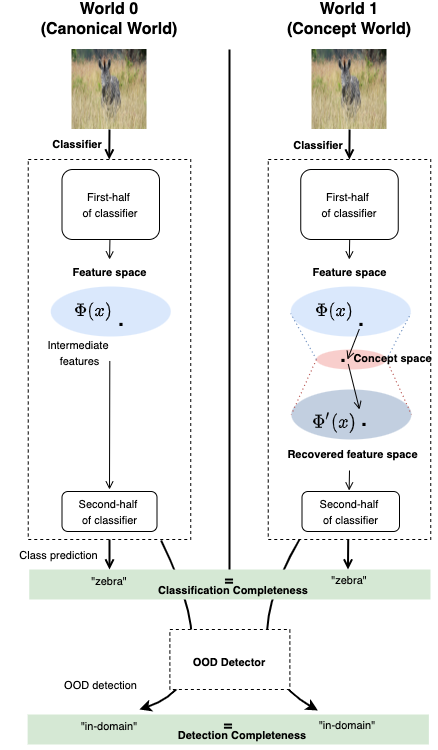
\includegraphics[width=0.45\textwidth]{figures/completeness.png}
% 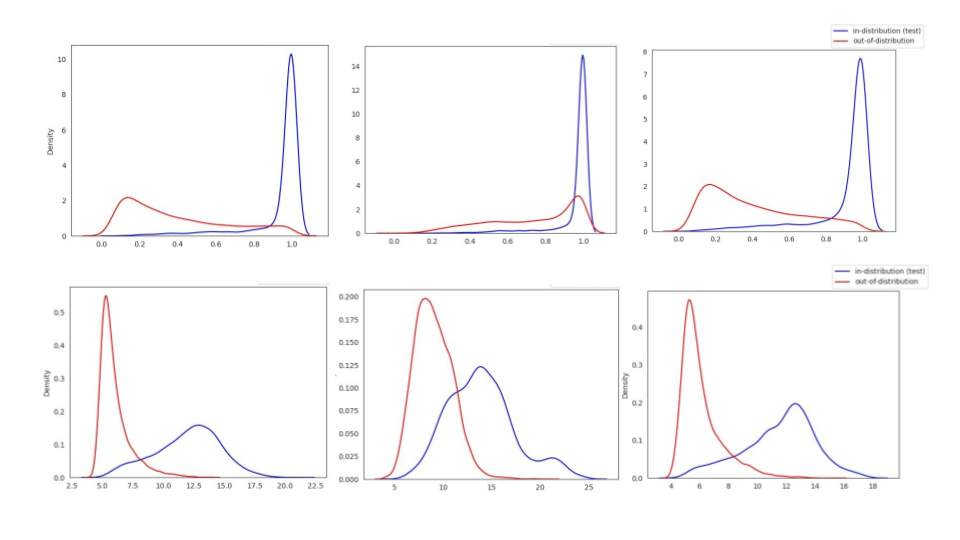
\includegraphics[scale=0.24]{figures/distribution.png}
% %\vspace{-2mm}
% \caption{Blue line is the estimated density of outputs from $\calD$ given ID test data (AwA), and red line is that of OOD test data (SUN). DNN classifier is Inception-V3 trained with AwA dataset.
% \textbf{First row}: distributions of outputs from MSP detector \citep{hendrycks2016msp}. 
% \textbf{Second row}: distributions of outputs from Energy detector \citep{liu2020energy}.
% \textbf{Left}: Target distribution of $S(\bfx, \bff)$ in canonical world. 
% \textbf{Mid}: Distribution of $S(\bfx, \fcon)$ in concept world, using concepts learned by \citep{yeh2020completeness}.
% \textbf{Right}: Distribution of $S(\bfx, \fcon)$ in concept world, using concepts learned by our framework.}
% \vspace{-5mm}
% \label{fig:score-distribution}
% \end{figure}
%

% \mypara{Limitations of Prior Work for OOD detectors.} 
While the objective (\ref{equ: baseline}) of \citeauthor{yeh2020completeness} can learn a set of sufficient concepts that have a high classification completeness score, we find that it does not necessarily replicate the per-instance prediction behavior of the classifier in the concept world. 
Specifically, there can be discrepancies in the reconstructed feature representation, whose effect propagates through the remaining part of the classifier. %to the output of the classifier.
% For instance, the empirical distribution of the prediction logits (pre-softmax layer) for both ID and OOD data based on the reconstructed feature representations could be very different from that based on the original feature representations.
Since many widely-used OOD detectors rely on the feature representations and/or the classifier's predictions, this discrepancy in the existing concept learning approaches makes it hard to closely replicate the OOD detector in the concept world (see Fig.~\ref{fig:score-distribution-msp}).
%
Furthermore, the scope of \citeauthor{yeh2020completeness} is confined to concept learning for explaining the classifier's predictions based on ID data, and there is no guarantee that the learned concepts would be useful for explaining an OOD detector. 
% In fact, the distribution of concept scores from ID and OOD data could be quite different (see Fig.~\ref{fig:score-distribution}).
% We illustrate this effect with a concrete example in Section~\ref{subsec:results}, when comparing the concept-score distributions from ID and OOD data based on the method of \citet{yeh2020completeness} and the proposed method.
%
To address these gaps, we propose a general method for concept learning that complements prior work by imposing additional instance-level constraints on the concepts, and by considering both the OOD detector and OOD data.
%
% We propose a general method for concept learning that overcomes the above gaps. Our method complements prior work by imposing additional instance-level constraints on the concepts, and by considering both the OOD detector and OOD data, as explained below.

\iffalse

% Earlier version
Unfortunately, there is a caveat with their approach.
Eqn. (\ref{equ: baseline}) may encourage the concepts to have high classification completeness score (defined in Eqn. (\ref{equ: completeness-classification})), but their concepts may fail to reduce the gap between canonical world and concept world genuinely. \ryan{By ensuring that they achieve an}
\textit{accurate reconstruction} of $\hat{\calZ}$
, the resulted concept scores would be sufficient enough to recover the accuracy of $\bff$ in expectation, but it is unclear whether the per-instance behavior of $\bff$ (and moreover, $\calD$ that runs based on $\bff$) is genuinely imitated.
To be more specific, $\bfC$ would be a set of $m$ principal vectors 
the set of concept vectors
$m$ unit vectors that fully span the space supported by $\{\bfphi(\bfx_1), \cdots, \bfphi(\bfx_{\Nintr})$.
usually not independent to each other (\eg concept "Greenery" is negatively related to concept "Sea").
have no guarantee on how \textit{accurate} the concepts are in explaining the classifier and the OOD detector.
% The reason we should care about in instance-level behavior of $\bff$ and $\calD$ in concept world is as follows. 
Besides, since the focus of \citep{yeh2020completeness} is initially confined to studying the utility of concepts for classifier with ID data, there is no guarantee for the utility of concepts for OOD detector explanations and in fact they distributions in concept space could be quite different for both ID and OOD data. We illustrate this effect with a concrete example in Section~\ref{subsec:results} when comparing the score distributions between ID and OOD on Yeh et al.~\citep{yeh2020completeness} and our approach to evaluate our reconstructed feature space $\hat{\calZ}$. To this end, we propose a general framework for concept learning that complements the previous works by additionally imposing instance-level requirements for concepts, and taking OOD data and OOD detector into consideration.

\fi

% \begin{equation}
% \label{equ: baseline+l2}
%     \argmax_{\bfC, g} \, \text{log} \proba_{(\bfx, y) \sim D^{train}_{in}}[\, h_{y}(\hat{\phi}_{g, \bfC}(\bfx))] + \lambda_1 \cdot R_{coherency}(\bfC) + \lambda_2 \cdot
%     \expec_{\bfx \sim D_{train}^{in}}||\phi(\bfx) - \hat{\phi}_{g, \bfC}(\bfx))||_2
% \end{equation}
% \begin{equation}
% \label{equ: baseline+score}
%     \argmax_{\bfC, g} \, \log \proba_{(\bfx, y) \sim D^{train}_{in}}[\, h_{y}(\hat{\phi}_{g, \bfC}(\bfx))] ~+~ \lambda\, R_{coherency}(\bfC) ~-~ \alpha \expec_{\bfx \sim D_{train}^{in}} (\mathcal{D}(h(\hat{\phi}_{g, \bfC}(\bfx))) - \mathcal{D}(f(\bfx)))^2
% \end{equation}

% Let $D^{train} = \{D_{\text{in}}^{train} \cup D_{\text{out}}^{train}\}$, and data is drawn as $(\bfx, s) \sim D^{train}$ where $s \in \{0, 1\}$ is the groundtruth label of OOD detection.
%
% \begin{equation}
% \label{equ: baseline+separability}
%     \argmax_{\bfC, g} \, \log \proba_{(\bfx, y) \sim D^{train}_{in}}[\, h_{y}(\hat{\phi}_{g, \bfC}(\bfx))] ~+~ \lambda\, R_{coherency}(\bfC) ~+~ \beta \expec_{\bfx \sim D^{train}} J(\bfC)
% \end{equation}
%

% \ap{Footenotetext for the algorithm is not appearing on the correct page. We may need to move it up or down when we get closer to the final draft.}

\mypara{Concept Learning Objective.}
We define a concept learning objective that aims to find a set of concepts $\bfC$ and a mapping $\bfg$ that have the following properties: 1) high detection completeness w.r.t the OOD detector; 2) high classification completeness w.r.t the DNN classifier; and 3) high separability in the concept-score space between detected-ID data and detected-OOD data.

\begin{figure*}[t]
  \centering
  \begin{subfigure}{0.32\linewidth}
    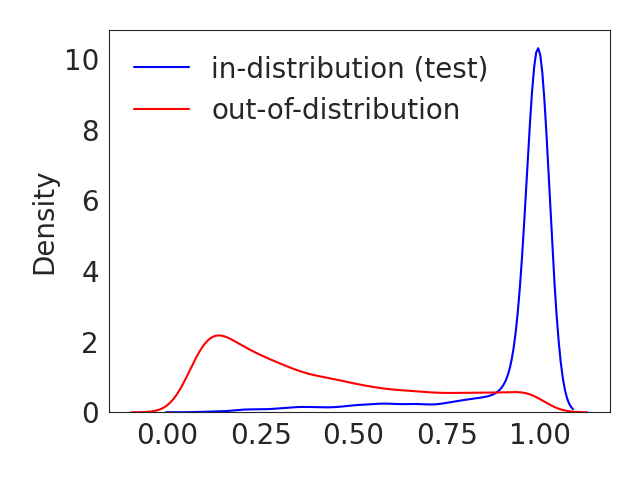
\includegraphics[width=\textwidth]{figures/distr_msp_target.png}
    \caption{\small Empirical distribution of $S(\bfx, \bff)$ from the target detector.}
    \label{fig:short-a}
  \end{subfigure}
  \hfill
  \begin{subfigure}{0.32\linewidth}
    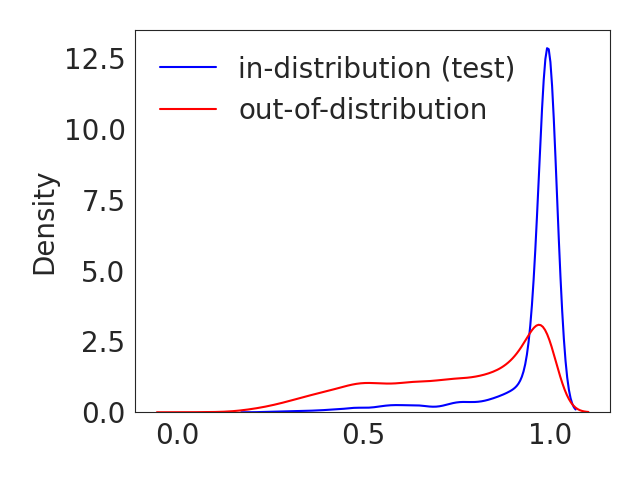
\includegraphics[width=\textwidth]{figures/distr_msp_yeh.png}
    \caption{\small Distribution of $\Scon(\bfx, \bff)$ using the concepts learned by \citet{yeh2020completeness}.}
    \label{fig:short-b}
  \end{subfigure}
  \hfill
  \begin{subfigure}{0.32\linewidth}
    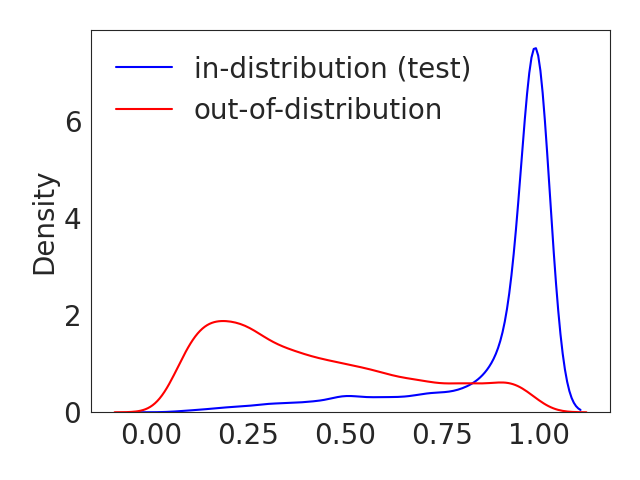
\includegraphics[width=\textwidth]{figures/distr_msp_ours.png}
    \caption{\small Distribution of $\Scon(\bfx, \bff)$ using the concepts learned by our method.}
    \label{fig:short-c}
  \end{subfigure}
  \caption{\small Empirical distribution of: \textbf{(a)} MSP detector score $S(\bfx, \bff)$ in the canonical world vs. \textbf{(b, c)} Reconstructed $\Scon(\bfx, \bff)$ in the concept world using the concepts learned by \citet{yeh2020completeness} and our method.
  Concepts learned by~\citet{yeh2020completeness} have $\eta^{}_{\bff} = 0.977, ~\eta^{}_{\bff, S}(\bfC) = 0.782$, while the concepts learned by our method $(\lambda_\textrm{mse} = 10, \lambda_\textrm{norm} = 0.1, \lambda_\textrm{sep} = 50)$ have $\eta^{}_{\bff} = 0.984, ~\eta^{}_{\bff, S}(\bfC) = 0.961$. 
  The AwA test set and the \texttt{SUN} dataset are used as ID (blue) and OOD (red) respectively.
    % Comparison is made between AwA test set (ID; blue) vs. \texttt{SUN} (OOD; red).
    }
    \vspace{-.1in}
\label{fig:score-distribution-msp}
\end{figure*}

% between the samples detected as ID and the samples detected as OOD by the detector. 
Inspired by recent works on transferring feature information from a teacher model to a student model~\citep{hinton2015distilling,zhou2018rocket},
% Recall that $\bfC$ projects from the original feature-representation space $\calZ$ to the concept-score space, which is then mapped to the reconstructed feature-representation space $\hat{\calZ}$ by $\bfg$.
we encourage accurate reconstruction of $\hat{\calZ}$ based on the concept scores by adding a regularization term that is the squared $\ell_2$ distance between the original and reconstructed representations $\,J_{\textrm{norm}}(\bfC, \bfg) ~=~ \expec_{\bfx \sim \Pin} \|\bfphi(\bfx) \,-\, \recphi(\bfx)\|^2\,$.
%
% \begin{align}
% \label{equ:regularizer_norm}
%     J_{\textrm{norm}}(\bfC, \bfg) ~=~ \expec_{\bfx \sim \Pin} \|\bfphi(\bfx) \,-\, \recphi(\bfx)\|^2.
% \end{align}
%
In order to close the gap between the scores of the OOD detector in the concept world and canonical world on a per-sample level, we introduce the following mean-squared-error (MSE) based regularization:
\begin{align}
\label{equ:regularizer_mse}
    J_{\textrm{mse}}(\bfC, \bfg) ~&=~ \expec_{\bfx \sim \Pin} \big( S(\bfx, \bfh \circ \recphi) - S(\bfx, \bff) \big)^2 \nonumber \\
    &~+~ \expec_{\bfx \sim \Pout} \big( S(\bfx, \bfh \circ \recphi) - S(\bfx, \bff) \big)^2 .
\end{align}
MSE terms are computed with both the ID and OOD data because we want to ensure that the ROC curve corresponding to both the score functions are close to each other (which requires OOD data).
Finally, we include a regularization term to maximize the separability metric between the detected-ID and detected-OOD data in the concept-score space, resulting in our final concept learning objective:
% We use the separability metric discussed in Section~\ref{sec:separability_score} directly as the regularization term since it is differentiable and tractable to optimize via gradient updates.
% With all regularization terms considered, 
%\vspace{-3mm}
\begin{align}
\label{equ: concept learning}
&\argmax_{\bfC, \bfg}  \expec_{(\bfx, y) \sim \Pin}\!\!\big[ \log h_y(\bfg(\VC(\bfx))) \big] ~+~ \lambda_{\textrm{expl}}\, R_{\textrm{expl}}(\bfC) \nonumber \\ 
    &-~ \lambda_{\textrm{mse}}\, J_{\textrm{mse}}(\bfC, \bfg) ~-~ \lambda_{\textrm{norm}}\, J_{\textrm{norm}}(\bfC, \bfg) ~+~ \lambda_{\textrm{sep}}~J_{\textrm{sep}}(\bfC).
\end{align}
The $\lambda$ coefficients are non-negative hyper-parameters that are further discussed in Section~\ref{subsec:results}.
We note that both $J_{\textrm{mse}}(\bfC, \bfg)$ and $J_{\textrm{sep}}(\bfC)$ depend on the OOD detector~\footnote{This dependence may not be obvious for the separability term, but it is clear from its definition.}.
% In case of the latter, this is clear from its definition, but may not obvious.
% The sign on the $\ell_2$ norm-based regularization and the MSE regularization terms is negative since we aim to minimize them.
% We use stochastic gradient descent-based optimization with adaptive learning rate (specifically Adam~\citep{kingma2014adam}) to solve the learning objective.
We use the SGD-based Adam optimizer~\citep{kingma2014adam}) to solve the learning objective.
The expectations involved in the objective terms are calculated using sample estimates from the training ID and OOD datasets. 
Specifically, $\Dintr$ and $\Douttr$ are used to compute the expectations over $\Pin$ and $\Pout$, respectively.
% The expectations involved in each of the terms in the objective are calculated using sample estimates from the training ID and OOD datasets. 
% Specifically, $\Dintr$ is used to compute the expectation over $\Pin$, and $\Douttr$ is used to compute the expectation over $\Pout$.
Our complete concept learning is summarized in Algorithm \ref{alg:concept_learning} (Appendix \ref{sec:appendix-algo}).



\iffalse

Detailed discussion of concept scores:

\mypara{Concept Scores.}
We start by formalizing how to compute a representative score for concepts given an input, which will be used for evaluation in Section \ref{sec:completeness_score} and Section \ref{sec:separability_score}.
We refer the reader to Section~\ref{sec:concept_projection}, which introduced a projection matrix $\bfC \in \reals^{d_\ell \times m}$ that maps $\bfphi(\bfx)$ to $\bfv_{\bfC}(\bfx)$ and consists of $m$ unit (column) concept vectors $\,\bfC := [\bfc_1 \cdots \bfc_m]$. 
The inner product between the feature representation and a concept vector quantifies how close the input is to the given concept, and this is referred to as the {\em concept score}. \ap{Does this need a cite? or is this our term?}
Specifically, the concept score corresponding to concept $i$ is $\bfv_{\bfc_i}(\bfx) = \langle \bfphi(\bfx), \bfc_i \rangle \in \reals^{a_\ell b_\ell}$, which is the $a_\ell \times b_\ell$ times concatenation over the standard inner-products (between vectors) $\,\langle \bfphi^{p,q}(\bfx), \bfc_i \rangle \in \reals, ~\forall p, q \in [a_\ell] \times [b_\ell]$, where $\bfphi^{p,q}$ is the feature representation corresponding to the $(p, q)$-th patch of input $\bfx$ (\ie receptive field).
That is, $\bfv_{\bfc_i}^{(p,q)}(\bfx)$ is the concept score of $(p, q)$-th patch of $\bfx$ with respect to $i$-th concept, and if it is a large positive (or negative) value, then the corresponding part of input is positively (or negatively) aligned with the concept.
The vector of concept scores from all the concepts is defined simply as the concatenation of the individual concept scores, \ie $\VC(\bfx)^T = [\bfv_{\bfc_1}(\bfx)^T, \cdots, \bfv_{\bfc_m}(\bfx)^T] \in \reals^{a_\ell b_\ell m}$.

% When $p = q = 1$ for fully-connected layers (\ie the receptive field of $\bfphi$ corresponds to the entire input $\bfx_i$), $\langle \bfphi(\bfx_i),~\bfc_j \rangle$ is a scalar concept score that represents the input.
% On the other hand, when $p, q > 1$, to obtain a scalar concept score for a given input, we take the maximum absolute concept score across the $p \times q$ patches, corresponding to $p \times q$ feature representations.
% To define the overall closeness of an input $\bfx_i$ and the concept $\bfc_j$ with a scalar concept score, we take the maximum absolute concept score across the $p \times q$ patches of $\bfx_i$.

\ap{Are p and q referring to the patch position? If so, why are (1,1), (1, -), and (-, 1) excluded by p, q > 1?}

When $p, q > 1$ (unless a fully-connected layer is of interest), where the receptive field of $\bfphi$ corresponds to the entire input $\bfx_i$), we also define a dimension-reduced version of the concept score vector that takes the maximum of the inner-product over each $a_\ell \times b_\ell$ patch (instead of concatenating them) as follows: $\TVC(\bfx)^T = [\widetilde{v}_{\bfc_1}(\bfx), \cdots, \widetilde{v}_{\bfc_m}(\bfx)] \in \reals^m$, where $\widetilde{v}_{\bfc_i}(\bfx) = \max_{p, q} |\langle \bfphi^{p,q}(\bfx), \bfc_i \rangle| \in \reals$.
% The intuition behind taking a maximum score across the patches of input is as follows.
This reduction operation is done to capture the most important correlations from each patch.
Suppose $\bfc_j$ represents a striped pattern and $\bfx_i$ is an image of a zebra standing on grass.
The patch of greenery background should get a low concept score, while a patch of the zebra's body should get high concept score.
% As the defining score for the stripe concept, we decide to take the score from the patch of zebra's body, out of all patches constituting the entire input image.
Out of all the patches constituting the input image, we take the maximum score (likely) corresponding to a patch of the zebra's body as the defining score for the striped concept.

Based on the concept scores and data defined as above, we elaborate the evaluation criteria of concepts for the purpose of OOD detector explanation in Section \ref{sec:completeness_score} and Section \ref{sec:separability_score}, followed by a general learning algorithm to discover concepts that satisfy the criteria in Section \ref{sec:concept_learning}.


\fi


% \begin{figure}[tbp]
% \centering
% \subfloat[MSP, target \label{fig:distr_msp_target}]{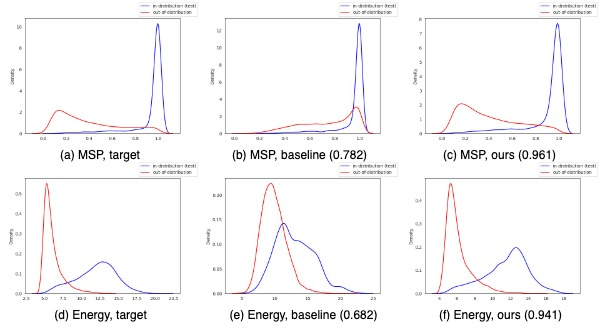
\includegraphics[width=0.3\textwidth]{figures/score_distribution.jpg}}\hfill
% \subfloat[Energy, ours\label{fig:distr_energy_ours}]{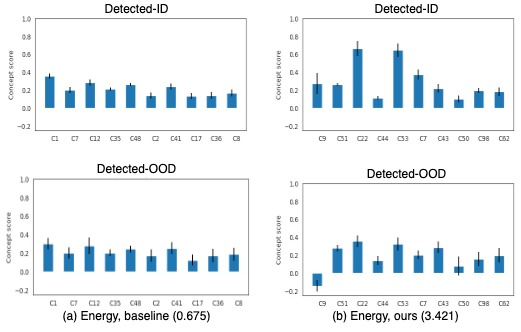
\includegraphics[width=0.3\textwidth]{figures/visual_dstinct.jpg}}
% \caption{
% \small \textbf{Estimated density of the score $S(\bfx, \bff)$ from Energy detector ~\citep{liu2020energy}}. 
% ID data is AwA test set (blue) and OOD data is the SUN dataset ~\citep{xiao2010sun} (red).
% \textbf{Left}: Target distribution of $S(\bfx, \bff)$ in the canonical world. 
% \textbf{Mid}: Distribution of $\Scon(\bfx, \bff)$ in the concept world, using concepts learned by \citep{yeh2020completeness} ($\,\lambda_\textrm{mse} = \lambda_\textrm{norm} = \lambda_\textrm{sep} = 0$).
% \textbf{Right}: Distribution of $\Scon(\bfx, \bff)$ in the concept world, using concepts learned by our method ($\,\lambda_\textrm{mse} = 1, \lambda_\textrm{norm} = 0.1, \lambda_\textrm{sep} = 50$ for Energy).
% % For MSP we set $\lambda_\textrm{mse} = 10, \lambda_\textrm{norm} = 0.1, \lambda_\textrm{sep} = 0$, and 
% }
% \label{fig:score-distribution}
% %\vspace{-5mm}
% \end{figure}



\section{Experiments}
\label{subsec:results}

\iffalse

\begin{table*}[tb]
    \centering
    \begin{adjustbox}{width=1\columnwidth,center}
		\begin{tabular}{l|l|l|c|c|c|c|c|c|c|c}
			\toprule
			\multirow{3}{0.001\linewidth}{OOD detector} & \multirow{3}{0.10\linewidth}{Hyper-\\parameters} &
			\multirow{3}{0.05\linewidth}{ $\eta^{}_{\bff}(\bfC)$} & \multicolumn{8}{c}{OOD data} \\ \cline{4-11}
    		& & & \multicolumn{2}{c|}{\texttt{Places}} & \multicolumn{2}{c|}{\texttt{SUN}} & \multicolumn{2}{c|}{\texttt{Textures}} & \multicolumn{2}{c}{\texttt{iNaturalist}}\\ \cline{4-11}
    		& & & $\eta^{}_{\bff, S}(\bfC)$ & $J_{\textrm{sep}}(\bfC, \bfC')$ & $\eta^{}_{\bff, S}(\bfC)$ & $J_{\textrm{sep}}(\bfC, \bfC')$ & $\eta^{}_{\bff, S}(\bfC)$ & $J_{\textrm{sep}}(\bfC, \bfC')$ & $\eta^{}_{\bff, S}(\bfC)$ & $J_{\textrm{sep}}(\bfC, \bfC')$ \\ \hline \hline
			\multirow{4}{0.10\linewidth}{MSP \\ \citep{hendrycks2016msp}} 
			& $(0, 0, 0)$ & 0.977 \pm 0.0006 & 0.774 \pm 0.001 & 0.694 \pm 0.0153 & 0.782 \pm 0.001 & 1.088 \pm 0.0175 & 0.593 \pm 0.0013 & 0.765 \pm 0.0157 & 0.878 \pm 0.0008 & 1.075 \pm 0.0191\\
			& $(10, 0.1, 0)$ & \textbf{0.994} \pm 0.0004 & 0.947 \pm 0.0004 & 1.892 \pm 0.0393 & 0.946 \pm 0.0004 & 3.074 \pm 0.0531 & 0.920 \pm 0.0005 & 3.577 \pm 0.1292 & \textbf{0.967} \pm 0.0004 &  \\
			& $(0, 0, 50)$ & 0.980 \pm 0.0005 & 0.814 \pm 0.0008 & 2.533 \pm 0.0714 & 0.816 \pm 0.0009 & 4.295 \pm 0.1048 & 0.773 \pm 0.0010 & 3.147 \pm 0.2076 & 0.864 \pm 0.0007 &\\
			& $(10, 0.1, 50)$ & 0.984 \pm 0.0004 & \textbf{0.960} \pm 0.0004 & 2.756 \pm 0.0854 & \textbf{0.961} \pm 0.0005 & 4.442 \pm 0.0830 & \textbf{0.937} \pm 0.0004 & \textbf{0.439} \pm 0.0175 & 0.946 \pm 0.0004 & \textbf{0.795} \pm 0.0473\\ \hline 
			\multirow{4}{0.10\linewidth}{ODIN \\ \citep{liang2018ODIN}} 
			& $(0, 0, 0)$ & 0.977 \pm 0.0006 & 0.742 \pm 0.0011 & 0.0 & 0.745 \pm 0.0010 & 0.0 & 0.618 \pm 0.0013 & 0.0 & 0.906 \pm 0.0007 & 0.0\\
			& $(\expnum{1}{+8}, 0.1, 0)$ & \textbf{0.994} \pm 0.0004 & 0.951 \pm 0.0004 & -0.118 \pm 0.0099 & 0.958 \pm 0.0004 & -0.054 \pm 0.0119 & 0.934 \pm 0.0004 & -0.245 \pm 0.0133 & 0.935 \pm 0.0004 & -0.345 \pm 0.0153\\
			& $(0, 0, 50)$ & 0.987 \pm 0.0004 & 0.899 \pm 0.0007 & \textbf{0.492} \pm 0.0215 & 0.911 \pm 0.0006 & 0.520 \pm 0.0187 & 0.793 \pm 0.0008 & 0.422 \pm 0.0175 & 0.971 \pm 0.0004 & 0.318 \pm 0.0343\\
			& $(\expnum{1}{8}, 0.1, 50)$ & 0.991 & \textbf{0.973} & 0.355 & \textbf{0.969} & \textbf{0.356} & \textbf{0.945} & 0.405 & \textbf{0.982} & 0.308 \\ \hline
			\multirow{4}{0.10\linewidth}{General-ODIN \\ \citep{hsu2020GeneralizedODIN}} 
			& $(0, 0, 0)$ & 0.990 \pm 0.0004 & 0.869 & 0.0 & 0.869 & 0.0 & 0.850 & 0.0 & 0.981 & 0.0\\
			& $(10^8, 0.1, 0)$ & \textbf{0.994} \pm 0.0004 & 0.951 \pm 0.0006 & 0.161 & 0.959 & 0.215 & 0.936 & 0.411 & 0.936 & 0.151\\
			& $(0, 0, 50)$ & 0.987 & 0.899 & \textbf{0.373} & 0.911 & 0.342 & 0.790 & \textbf{0.414} & 0.970 & \textbf{0.337}\\
			& $(10^8, 0.1, 50)$ & 0.991 & \textbf{0.973} & 0.355 & \textbf{0.969} & \textbf{0.356} & \textbf{0.945} & 0.405 & \textbf{0.982} & 0.308 \\ \hline
			\multirow{4}{0.10\linewidth}{Energy \\ \citep{liu2020energy}} 
			& $(0, 0, 0)$ & 0.977 \pm 0.0006 & 0.671 \pm 0.0012 & 0.0 & 0.682 \pm 0.0012 & 0.0 & 0.557 \pm 0.0014 & 0.0 & 0.871 \pm 0.0007 & 0.0\\
			& $(1. 0.1, 0)$ & \textbf{0.993} \pm 0.0005 & \textbf{0.965} \pm 0.0004 & 0.191 \pm 0.0126 & \textbf{0.963} \pm 0.0004 & 0.326 \pm 0.0133 & \textbf{0.960} \pm 0.0003 & 0.110 \pm 0.0117 & \textbf{0.949} \pm 0.0004 & 0.770 \pm 0.0334\\
			& $(0, 0, 50)$ & 0.987 \pm 0.0005 & 0.779 \pm 0.0010 & 0.4703 \pm 0.0199 & 0.793 \pm 0.0009 & 0.427 \pm 0.0153 &  0.767 \pm 0.0010 & 0.531 \pm 0.0184 & 0.911 \pm 0.0006 & 0.263 \pm 0.0297 \\
			& $(1, 0.1, 50)$ & 0.980 \pm 0.0005 & 0.943 \pm 0.0005 & 0.534 \pm 0.0218 & \textbf{0.941} \pm 0.0005 & 0.534 \pm 0.0175 & 0.936 \pm 0.0005 & 0.658 \pm 0.0212 & 0.927 \pm 0.0005 & 0.291 \pm 0.0319 \\ \hline
			\multirow{4}{0.10\linewidth}{Mahal \\ \citep{lee2018mahalanobis}} 
			& $(0, 0, 0)$ & 0.990 & 0.860 & 0.0 & 0.860 & 0.0 & 0.831 & 0.0 & 0.972 & 0.0 \\
			& $(0.1, 0.1, 0)$ & \textbf{0.994} & 0.962 & 0.153 & 0.963 & 0.176 & 0.962 & 0.351 & 0.955 & 0.169\\
			& $(0, 0, 50)$ & 0.985 & 0.850 & \textbf{0.430} & 0.883 & 0.362 & 0.774 & \textbf{0.429} & 0.926 & \textbf{0.386} \\
			& $(0.1, 0.1, 50)$ & 0.991 & \textbf{0.971} & 0.370 & \textbf{0.970} & \textbf{0.388} & \textbf{0.970} & 0.397 & \textbf{0.972} & 0.351 \\ \bottomrule
		\end{tabular}
	\end{adjustbox}
	\caption[]{\small \textbf{Results of concept learning with different parameter settings across various OOD detectors and OOD datasets.} 
% 	$\bfC'$ denotes a set of concepts discovered by baseline \citep{yeh2020completeness} (\ie $\lambda_\textrm{mse} = 0, \lambda_\textrm{norm} = 0, \lambda_\textrm{sep} = 0$).
	Hyperparameters are in the order of $(\lambda_\textrm{mse}, \lambda_\textrm{norm}, \lambda_\textrm{sep})$. Larger values are better for all the metrics. \textbf{Bold} numbers indicate the best results (across the rows) for a given OOD detection method and dataset. Note that by definition of $J_{\textrm{sep}}(\bfC, \bfC')$ (Eqn. \ref{eq:relative-separability}), the relative concept separability of the baseline~\citep{yeh2020completeness} is always $0$, \ie $J_{\textrm{sep}}(\bfC', \bfC') = 0$.}
	\label{tab:concept-learning-results}
\end{table*}

\fi

\iffalse

We perform experiments to evaluate the proposed method and address the following questions:
\begin{enumerate}[start=1,label={\bfseries Q\arabic*.}]
    \item \label{Q1} Does our concept learning objective effectively encourage concepts to have the desired properties of detection completeness and concept separability?
    \item \label{Q2} Are the proposed evaluation metrics well-aligned with the interpretability of the resulting concept-based explanations?
    % Are the proposed evaluations metrics beneficial for better interpretability of resulting concept-based explanations?
    % \jayaram{Are the proposed evaluation metrics effective at providing better interpretability for the resulting concept-based explanations?}
    % Does a high detection completeness score of concepts imply a more accurate explanaation of the OOD detector? Does better concept separability lead to a more distinctive explanation between ID- and OOD-detected data?
    \item \label{Q3} Given concepts learned by our approach, what insights can we provide for the OOD detector?
\end{enumerate}

Our main findings are summarized as follows:
\begin{enumerate}[start=1,label={\bfseries A\arabic*.}]
    \item In accordance with our design intention, our $\ell_2$ norm-based regularization and MSE regularization not only improve the detection completeness by large margin, but also the classification completeness even further. 
    The proposed separability regularization effectively improves concept separability, and when these three terms are used together in concept learning objective, we can achieve the highest detection completeness and concept separability (see Table \ref{tab:concept-learning-results}).
    \item Concepts with a high completeness score enable to mimic the original behavior of the OOD detector more precisely, hence leading to more \textit{accurate} explanations based on the concepts (see Fig. \ref{fig:score-distribution}). 
    Also, concepts with a higher concept separability score lead to more \textit{visually-distinctive} interpretations between ID and OOD data by having more distinguishable concept-score patterns (see Fig. \ref{fig:high_separa_interpretatbility}).
    % Concepts learned by our method enable more \textit{accurate}, and more \textit{visually distinctive} interpretations, compared to the concepts learned by the baseline method (\citep{yeh2020completeness}).
    \item We can rank the importance of each concept towards OOD detection using the Shapley value modified with our per-class detection completeness metric. 
    When the concepts are only targeted at explaining the DNN classifier (as in the baseline \citep{yeh2020completeness}), the behavior of the OOD detector is merely described by the common set of concepts that are important for the DNN classifier.
    On the other hand, when not only the DNN classifier but also the OOD detector is taken into consideration during concept learning (\ie our method), we obtain a more diverse and expanded set of concepts, and different concepts play a major role in interpreting the classification and detection results (see Fig. \ref{fig:shap_buffalo}). 
    % identify based on what concepts an OOD detector makes decisions.
    % We can identify the top concepts that contribute to the OOD detector's decisions using  
\end{enumerate}



\fi

In this section, we conduct experiments to evaluate the proposed method and show that: 1) the learned concepts satisfy the desiderata of completeness and separability across popular off-the-shelf OOD detectors and real-world datasets. 2) the learned concepts can be combined with a Shapley value to provide insightful visual explanations that can help understand the predictions of an OOD detector. 
The code for our work can be found at \url{https://github.com/jihyechoi77/concepts-for-ood}.
% In this section, we conduct experiments to show that our method can learn concepts that satisfy the desiderata of completeness and separability across popular off-the-shelf OOD detectors and real-world datasets.
% We start the experimental section by answering the fundamental question: \textit{can our concept learning framework find a good set of concepts that satisfy the desiderata of completeness and separability as intended?}
% We observe that the resulting concepts have high completeness and separability scores when evaluated with real-world ID and OOD images, and targeted for popular off-the-shelf OOD detectors.

\subsection{Experimental Setup}
\label{sec:setup}
% We briefly describe the experimental setup here and provide additional details in Appendix \ref{sec:appendix-implementation-details}.
% We briefly describe the setup of our experiments to address the above questions. See Appendix \ref{sec:appendix-implementation-details} for further details.
% For reproducibility, we have released our anonymized source code ~\footnote{\url{https://anonymous.4open.science/r/Concept-For-OOD-CE1B/}}.

\mypara{Datasets.} For the ID dataset, we use Animals with Attributes (AwA) \citep{xian2018awa} with 50 animal classes, and split it into a train set (29841 images), validation set (3709 images), and test set (3772 images).
We use the MSCOCO dataset \citep{lin2014mscoco} as the auxiliary OOD dataset $\Douttr$ for training and validation.
For the OOD test dataset $\Doutte$, we follow the literature of large-scale OOD detection \citep{Huang_MOS} and use three different image datasets: \texttt{Places365} \citep{zhou2017places}, \texttt{SUN} \citep{xiao2010sun}, and \texttt{Textures} \citep{cimpoi2014textures}.
% , \texttt{iNaturalist} \citep{van2018inaturalist}; all resized to the input size $224 \times 224$.

% \textbf{OOD detector.} We apply our general approach to intepret four popular OOD detection methods in the literature: MSP \citep{hendrycks2016msp}, ODIN \citep{liang2018ODIN}, Energy \citep{liu2020energy} and Mahalanobis \citep{lee2018mahalanobis} (henceforth abbreviated to Mahal).

% \jihye{real-world high resolution image data}
% \textbf{DNN classifier.} The OOD detectors are paired with the widely-used Inception-V3 model \citep{szegedy2016inception-v3} (following the common setup in prior works \citep{yeh2020completeness, ghorbani2019ace, koh2020concept-bottleneck, kim2018tcav}) trained on AwA, which yields $0.921$ test accuracy. 


\mypara{Models.}
We apply our framework to interpret five prominent OOD detectors from the literature: MSP~\citep{hendrycks2016msp}, ODIN~\citep{liang2018ODIN}, Generalized-ODIN~\citep{hsu2020GeneralizedODIN}, Energy~\citep{liu2020energy}, and Mahalanobis~\citep{lee2018mahalanobis}.
The OOD detectors are paired with the widely-used Inception-V3 classifier~\citep{szegedy2016inception-v3} (following the setup in prior works~\citep{yeh2020completeness, ghorbani2019ace, kim2018tcav}), which has a test accuracy of $92.13 \%$ on the AwA dataset.
% trained on the Animals-with-Attributes (AwA) dataset~\citep{xian2018awa}, . 
% \subsection{Results}\label{subsec:results}
%
Additional details on the setup are given in Appendix~\ref{sec:appendix-implementation-details}.
% Codes for reproducibility are submitted as supplementary material.
 
\subsection{Effectiveness of the Concept Learning}
\label{sec:eval-concept}
% In this subsection, we elaborate on the experiments to answer the first question (Q1) on the effectiveness of our concept learning objective.
Table~\ref{tab:concept-learning-results-places} summarizes the results of concept learning for various combinations of the regularization coefficients ($\lambda_{\star}$) in Eqn (\ref{equ: concept learning}), including: \textbf{i)} baseline where all the coefficients are set to $0$ (first row); \textbf{ii)} only the terms directly relevant to detection completeness (\ie $J_{\textrm{norm}}(\bfC, \bfg)$ and $J_{\textrm{mse}}(\bfC, \bfg)$) are included (second row); \textbf{iii)} only the term responsible for concept separability $J_{\textrm{sep}}(\bfC)$ is included (third row); \textbf{iv)} all the regularization terms are included (fourth row).

From the table, we observe that the regularization terms encourage the learned concepts to satisfy the required desiderata of high completeness and concept separability scores.
% Given any OOD detector, we confirm the design of regularization terms to encourage the desiderata of concepts.
Having $\lambda_\textrm{mse} > 0\, \text{ and } \,\lambda_\textrm{norm} > 0$ always improves the detection completeness by a large margin (\ie row 2 compared to row 1), and having $\lambda_\textrm{sep} > 0$ significantly increases the concept separability (\ie row 3 compared to row 1).
% In accordance with our design intention, our $\ell_2$ norm-based regularization and MSE regularization not only improve the detection completeness by large margin, but also the classification completeness even further.
Importantly, when all the regularization terms are included, they have the best synergistic effect on the metrics. 
% More importantly, the three terms make the best synergy together in most cases.

\begin{table}[thb]
    \centering
    \begin{adjustbox}{width=1\columnwidth,center}
    % \begin{adjustbox}{width=1\textwidth,center}
		\begin{tabular}{l|l|c|c|c}
			\toprule
			OOD detector & $(\lambda_\textrm{mse}, \lambda_\textrm{norm}, \lambda_\textrm{sep})$ &
			$\eta^{}_{\bff}(\bfC) \uparrow$ & $\eta^{}_{\bff, S}(\bfC) \uparrow$ & $J_{\textrm{sep}}(\bfC, \bfC') \uparrow$ \\ \hline \hline
            \multirow{4}{0.10\linewidth}{MSP} 
			& $(0, 0, 0)$ & 0.977 $\pm$ 0.0006 & 0.774 $\pm$ 0.0010 & 0.694 $\pm$ 0.0153 \\
			& $(10, 0.1, 0)$ & \textbf{0.994} $\pm$ 0.0004 & \underline{0.947} $\pm$ 0.0004 & 1.892 $\pm$ 0.0393 \\
			& $(0, 0, 50)$ & 0.980 $\pm$ 0.0005 & 0.814 $\pm$ 0.0008 & \underline{2.533} $\pm$ 0.0714 \\
			& $(10, 0.1, 50)$ & \underline{0.984} $\pm$ 0.0004 & \textbf{0.960} $\pm$ 0.0004 & \textbf{2.756} $\pm$ 0.0854 \\ \hline
			%
            \multirow{4}{0.10\linewidth}{ODIN} 
			& $(0, 0, 0)$ & 0.977 $\pm$ 0.0006 & 0.742 $\pm$ 0.0011 & 0.444 $\pm$ 0.0119 \\
			& $(10^8, 0.1, 0)$ & \textbf{0.994} $\pm$ 0.0004 & \underline{0.951} $\pm$ 0.0004 & 1.166 $\pm$ 0.0303 \\
			& $(0, 0, 50)$ & 0.987 $\pm$ 0.0004 & 0.899 $\pm$ 0.0007 & \underline{1.785} $\pm$ 0.0669 \\
			& $(10^8, 0.1, 50)$ & \underline{0.991} $\pm$ 0,0005 & \textbf{0.973} $\pm$ 0.0009 & \textbf{1.813} $\pm$ 0.0268 \\ \hline
			%
            \multirow{4}{0.10\linewidth}{General-ODIN} 
			& $(0, 0, 0)$ & 0.988 $\pm$ 0.0004 & 0.769 $\pm$ 0.0004 & 0.506 $\pm$ 0.0165 \\
			& $(10^6, 0.1, 0)$ & \textbf{0.995} $\pm$ 0.0004 & \underline{0.951} $\pm$ 0.0006 & 1.461 $\pm$ 0.0321 \\
			& $(0, 0, 50)$ & 0.981 $\pm$ 0.0004 & 0.859 $\pm$ 0.0007 & \underline{1.814} $\pm$ 0.0685 \\
			& $(10^6, 0.1, 50)$ & \underline{0.990} $\pm$ 0.0005 & \textbf{0.971} $\pm$ 0.0010 & \textbf{1.835} $\pm$ 0.0669 \\ \hline
			%
            \multirow{4}{0.10\linewidth}{Energy} 
			& $(0, 0, 0)$ & 0.977 $\pm$ 0.0006 & 0.671 $\pm$ 0.0012 & 0.453 $\pm$ 0.0121 \\
			& $(1. 0.1, 0)$ & \textbf{0.993} $\pm$ 0.0005 & \textbf{0.965} $\pm$ 0.0004 & 1.266 $\pm$ 0.0319 \\
			& $(0, 0, 50)$ & \underline{0.987} $\pm$ 0.0005 & 0.779 $\pm$ 0.0010 & \textbf{1.920} $\pm$ 0.0725 \\
			& $(1, 0.1, 50)$ & 0.980 $\pm$ 0.0005 & \underline{0.943} $\pm$ 0.0005 & \underline{1.839} $\pm$ 0.0662 \\ \hline
			%
			\multirow{4}{0.10\linewidth}{Mahalanobis} 
			& $(0, 0, 0)$ & 0.990 $\pm$ 0.0007 & 0.715 $\pm$ 0.0011 & 0.571 $\pm$ 0.0110 \\
			& $(0.1, 0.1, 0)$ & \textbf{0.994} $\pm$ 0.0004 & \underline{0.950} $\pm$ 0.0009 & 1.532 $\pm$ 0.0351 \\
			& $(0, 0, 50)$ & 0.985 $\pm$ 0.0004 & 0.880 $\pm$ 0.0005 & \underline{2.550} $\pm$ 0.0681 \\
			& $(0.1, 0.1, 50)$ & \underline{0.992} $\pm$ 0.0006 & \textbf{0.961} $\pm$ 0.0005 & \textbf{2.616} $\pm$ 0.0857 \\ \bottomrule
		\end{tabular}
	\end{adjustbox}
	\caption[]{
	\small Concept learning results with different parameter settings across various OOD detectors, evaluated on AwA test set (ID) and \texttt{Places365} (OOD). 
% 	$\bfC'$ denotes a set of concepts discovered by baseline \citep{yeh2020completeness} (\ie $\lambda_\textrm{mse} = 0, \lambda_\textrm{norm} = 0, \lambda_\textrm{sep} = 0$).
% 	Larger values are better for all the metrics. 
Hyperparameters are set based on the scale of corresponding regularization terms for a specific choice of the OOD detector.
 Across the rows (for a given OOD detector), the best value is \textbf{boldfaced}, and the second best value is \underline{underlined}.
	The $95\%$ confidence intervals are estimated by bootstrapping the test set over $200$ trials. Complete results are given in Table~\ref{tab:concept-learning-results} in Appendix~\ref{sec:app_addi_results}.
% 	\textbf{Bold} numbers indicate the best results (across the rows) for a given OOD detection method and dataset. 
	%Note that by definition of $J_{\textrm{sep}}(\bfC, \bfC')$ (Eqn. \ref{eq:relative-separability}), the relative concept separability of the baseline~\citep{yeh2020completeness} is always $0$, \ie $J_{\textrm{sep}}(\bfC', \bfC') = 0$.
	}
\label{tab:concept-learning-results-places}
% \vspace{-.5in}
\end{table}
%


%\jihye{@Jayaram: not sure if mentioning this instance is necessary. } 
Consider the MSP detector for instance. The detection completeness increases from $0.774$ to $0.947$ with $\lambda_\textrm{mse} = 10, \lambda_\textrm{norm} = 0.1, \lambda_\textrm{sep} = 0$, and the concept separability increases from $0.694$ to $2.533$ with $\lambda_\textrm{mse} = 0, \lambda_\textrm{norm} = 0, \lambda_\textrm{sep} = 50$.
However, when all the terms are considered ($\lambda_\textrm{mse} = 10, \lambda_\textrm{norm} = 0.1, \lambda_\textrm{sep} = 50$), we achieve the best result of $\eta^{}_{\bff, S}(\bfC) = 0.960$ and $J_{\textrm{sep}}(\bfC, \bfC') = 2.756$. 
Results on other large-scale OOD datasets and ablation studies on the regularization terms can be found in Appendix \ref{sec:appendix-concept-learning-ablation}.

\iffalse

% \mypara{Metrics.}
% For each set of concepts learned with different OOD detectors and hyperparameters, we report the classification completeness $\eta^{}_{\bff}(\bfC)$, detection completeness $\eta^{}_{\bff, S}(\bfC)$, and the relative concept separability metric (defined below). 
In contrast to the completeness scores (\ie $\eta^{}_{\bff}(\bfC)$ and $\eta^{}_{\bff, S}(\bfC)$) that are almost always bounded to the range $[0, 1]$, it is hard to gauge the possible range of the separability score $J_{\textrm{sep}}(\bfC)$ (or $J^y_{\textrm{sep}}(\bfC)$) across different settings (datasets, classification models, and OOD detectors), and whether the value represents a significant improvement in separability.
Hence, in Table~\ref{tab:concept-learning-results-places}, we define and report the \textit{relative concept separability}, which captures the relative improvement in concept separability using concepts $\bfC$ compared to a different set of concepts $\bfC'$, as follows
% between two different sets of concepts, as follows
% \vspace{-1mm}
\begin{equation}
\label{eq:relative-separability}
J_{\textrm{sep}}(\bfC, \bfC') = \textrm{Median}\left( \left\{\frac{J^y_{\textrm{sep}}(\bfC) ~-~ J^y_{\textrm{sep}}(\bfC')}{J^y_{\textrm{sep}}(\bfC')}\right\}_{y=1}^L \right). 
\end{equation}
% This metric measures the median of the relative increase in the per-class separability using concepts $\bfC$, compared to that of using a different set of concepts $\bfC'$.
where $\bfC'$ is fixed as the set of concepts learned by the baseline of $\,\lambda_\textrm{mse} = \lambda_\textrm{norm} = \lambda_\textrm{sep} = 0$.
% The set of concept $\bfC$ is obtained via our concept learning objective, with various combinations of hyperparameter values.

\fi

Since the range of the separability score $J_{\textrm{sep}}(\bfC)$ (or $J^y_{\textrm{sep}}(\bfC)$) is not well defined, we report a \textit{relative concept separability} score that is easier to interpret, and defined as
\begin{equation}
\label{eq:relative-separability}
J_{\textrm{sep}}(\bfC, \bfC') = \textrm{Median}\left( \left\{\frac{J^y_{\textrm{sep}}(\bfC) ~-~ J^y_{\textrm{sep}}(\bfC')}{J^y_{\textrm{sep}}(\bfC')}\right\}_{y=1}^L \right). 
\end{equation}
It captures the relative improvement in concept separability using concepts $\bfC$, compared to a baseline set of concepts $\bfC'$ obtained by setting $\,\lambda_\textrm{mse} = \lambda_\textrm{norm} = \lambda_\textrm{sep} = 0$.
%

% We test how effectively our regularization terms improve detection completeness and concept separability, without sacrificing the classification completeness.
\mypara{Concepts good for the OOD detector are also good for the classifier, but not vice-versa.} 
Recall that the baseline $(\lambda_\textrm{mse} = \lambda_\textrm{norm} = \lambda_\textrm{sep} = 0)$ corresponds to the method of \citet{yeh2020completeness} where only the classifier is considered during the concept learning.
For any choice of OOD detector in Table~\ref{tab:concept-learning-results-places} and Table~\ref{tab:concept-learning-results} (in Appendix~\ref{sec:app_addi_results}), the concepts learned by our method always achieve higher scores even for classification completeness, compared to the baseline. 
In contrast, the baseline concepts for only the classifier have the lowest detection completeness and concept separability in all cases.
This may not be surprising since the scope of~\citet{yeh2020completeness} does not cover explaining detectors.
%Nonetheless, such observations become the supporting evidence of our motivation for this paper,
Nonetheless, such observations provide supporting evidence to motivate the need for our concept learning and novel metrics, indicating that {\em even if the concepts are sufficient to describe the DNN classifier, the same set of concepts may not be appropriate for the OOD detector.}

% We also observe that concept separability regularization term $J_{\textrm{sep}}(\bfC) > 0$ improves the relative concept separability, and when brought together with $J_{\textrm{norm}}(\bfC, \bfg)$ and  $J_{\textrm{mse}}(\bfC, \bfg) = 0$, can improve the detection completeness even further.
% By having $\lambda_\textrm{mse} > 0, \lambda_\textrm{norm} > 0, \lambda_\textrm{sep} = 0$, we observe that $\eta^{}_{\bff, S}(\bfC)$ is always improved by large margin compared to baseline.
%
% We observe that the relative concept separability $J_{\textrm{sep}}(\bfC, \bfC')$ is largest most often for the setting where $\lambda_\textrm{mse} = \lambda_\textrm{norm} = 0, \text{ and } \lambda_\textrm{sep} > 0$ (third row).
% However, the detection completeness does not improve and in some cases drops compared to the baseline setting, suggesting that there is a tradeoff between maximizing the detection completeness and concept separability.
%

% \jihye{For instance, given the ODIN detector and the \texttt{SUN} dataset, including our proposed regularization terms improves the detection completeness of concepts from $0.869$ to $0.969$, and the relative concept separability is increased by $0.356$, compared to when concepts are learned without the regularization terms.}
% In this setting, there is a slight decrease the relative concept separability compared to the case where only the regularization term $J_{\textrm{sep}}(\bfC)$ is included (third row). In other words, there is a tradeoff wherein we may have to sacrifice the concept separability a little in order to achieve the best possible detection completeness.


\iffalse
\mypara{Choice of Hyperparameters.}
\label{sec:hyperparameter}
In Table \ref{tab:concept-learning-results}, we set the values of $\lambda_{\textrm{norm}}, \lambda_{\textrm{mse}}$ and $\lambda_{\textrm{sep}}$ based on the scale of corresponding regularization terms in Eqn. (\ref{equ: concept learning}) (\ie $J_{\textrm{norm}}(\bfC, \bfg),  J_{\textrm{mse}}(\bfC, \bfg)$ and $ J_{\textrm{sep}}(\bfC)$, respectively) for a specific choice of the OOD detector.
Further investigation including an ablation study on each regularization term can be found in Appendix \ref{sec:appendix-concept-learning-ablation}.
From the ablation study, we note that there is a trade-off between concept separability and coherency (defined in Eqn. \ref{eq:coherency}).
This implies that high concept separability ensures easily distinguishable score patterns between detected-ID and detected-OOD inputs, but the discovered concepts may not be understandable to humans, hence the user needs to balance the degree of $\lambda_{\textrm{sep}}$ depending on the application of interest. 
\fi
% Interestingly, we observe that the concepts targeted for a particular type of OOD detector can also be applied to different types of OOD detectors (\ie the learned concepts exhibit transferability). 
% Transferability of concepts across different OOD detectors is also discussed in Appendix \ref{sec:appendix-concept-learning-transfer}.
\iffalse
\begin{figure}[h]
\centering
\subfigure{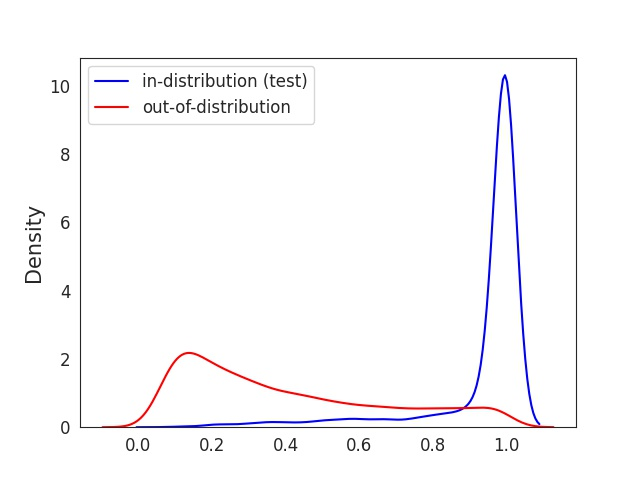
\includegraphics[width=0.31\textwidth]{figures/distr_msp_target.jpg}} 
\subfigure{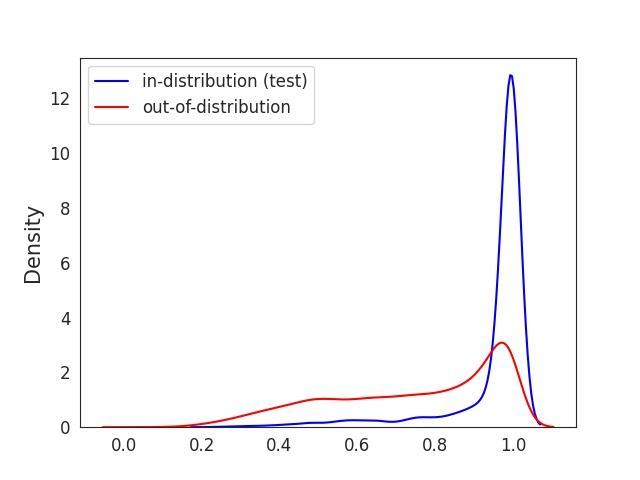
\includegraphics[width=0.31\textwidth]{figures/distr_msp_yeh.jpg}} 
\subfigure{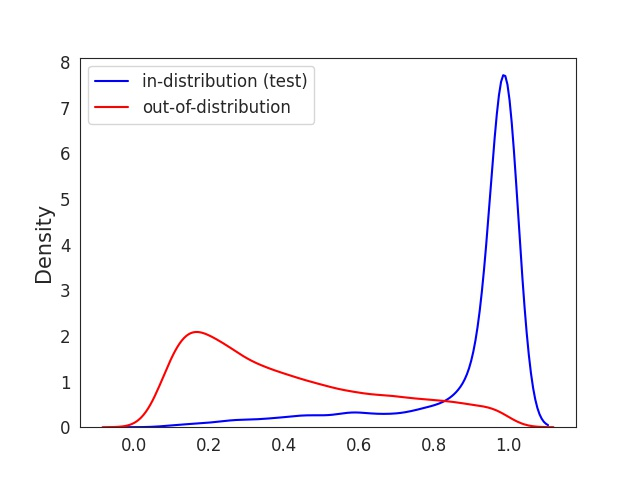
\includegraphics[width=0.31\textwidth]{figures/distr_msp_ours.jpg}} 
\caption{\textbf{Detection completeness and estimated density of OOD score $S(\bfx, \bff)$ from MSP detector.}
\textbf{Left}: Target distribution of $S(\bfx, \bff)$ in the canonical world. 
\textbf{Mid}: Distribution of $\Scon(\bfx, \bff)$ in the concept world, using concepts learned by \citep{yeh2020completeness} ($\,\lambda_\textrm{mse} = \lambda_\textrm{norm} = \lambda_\textrm{sep} = 0$).
\textbf{Right}: Distribution of $\Scon(\bfx, \bff)$ in the concept world, using concepts learned by our method ($\lambda_\textrm{mse} = 10, \lambda_\textrm{norm} = 0.1, \lambda_\textrm{sep} = 50$). Comparison is made between AwA test set (ID; blue) vs. SUN (OOD; red).}
\label{fig:score-distribution-msp}
\end{figure}
\fi

\begin{figure*}[hbt]
% \vspace{-5mm}
     
     \begin{subfigure}[b]{0.7\textwidth}
     \centering
     \begin{subfigure}{\textwidth}
         \centering
         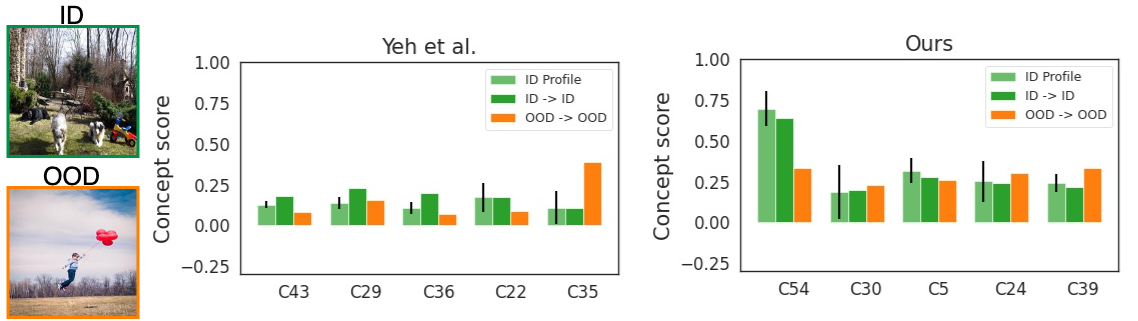
\includegraphics[width=\textwidth]{figures/fig3a.png}
         \caption{\small Correct detection: top collie image is correctly detected as ID (dark-green bar), and the bottom image is correctly detected as OOD (orange bar).}
         % ID (or OOD) dolphin image correctly detected as ID (or OOD).
         \label{fig:collie-correct}
     \end{subfigure}
     \\
     \begin{subfigure}{\textwidth}
         \centering
         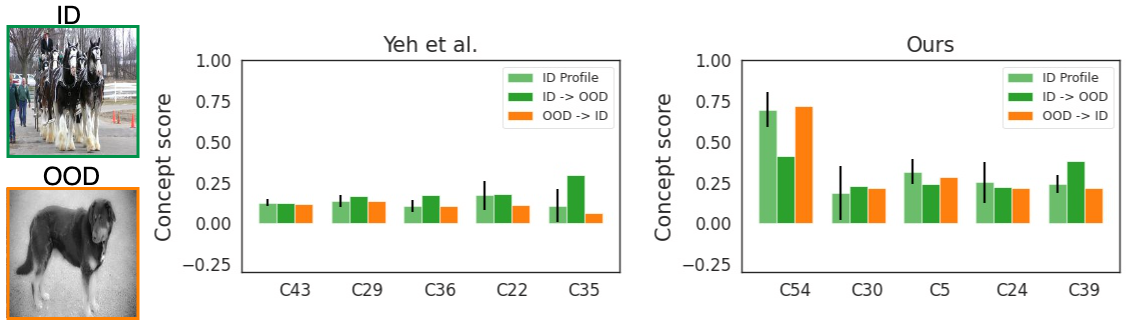
\includegraphics[width=\textwidth]{figures/fig3b.png}
         \caption{\small Wrong detection: top ID image is detected as OOD (dark-green bar), and the bottom OOD image is detected as ID (orange bar).}
         % ID (or OOD) dolphin image falsely detected as OOD (or ID).
         \label{fig:collie-wrong}
     \end{subfigure}
     \end{subfigure}
     \hspace{2mm}
     \begin{subfigure}[b]{0.23\textwidth}
         \centering
         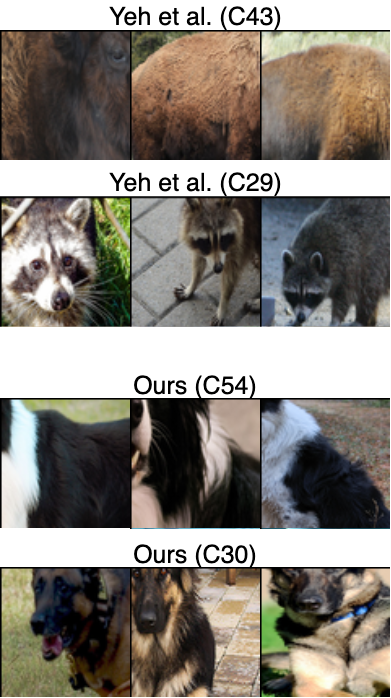
\includegraphics[width=\textwidth]{figures/fig3c.png}
         \caption{\small Visualization of top-2 important concepts found by the method of \citet{yeh2020completeness} and our method.}
         \label{fig:collie-concepts}
     \end{subfigure}
% \begin{subfigure}[b]{0.3\textwidth}
%     \centering
%     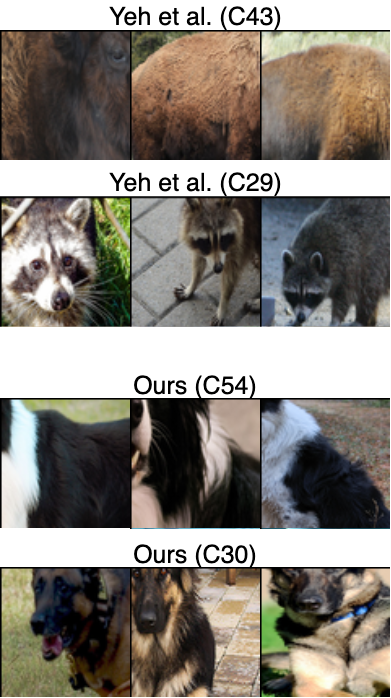
\includegraphics[width=0.9\textwidth]{figures/fig3c.png}
% \end{subfigure}
\caption{\small \textbf{Concept-based explanations for the Energy OOD detector using concepts learned by \citet{yeh2020completeness} vs. ours ($\lambda_\textrm{mse} = 1, \lambda_\textrm{norm} = 0.1, \lambda_\textrm{sep} = 10$)}. Images are randomly selected from the AwA test set (ID) and \texttt{Places} (OOD), and all of them are predicted to the class ``Collie''. Concept score patterns by \citet{yeh2020completeness} are not distinctive between detected-ID vs. detected-OOD (\ie dark-green bar and orange bar are not very different). Whereas, our concepts present very similar patterns to the ID profile (light-green bar) when input is detected as ID, and different from the ID profile when detected as OOD.
}
\label{fig:expl-energy-collie}

\end{figure*}




% \subsection{Interpretability of the Learned Concepts (Q2.)}
% \subsection{Our Metrics and Interpretability (Q2.).}
% \mypara{Reconstruction of $\hat{\calZ}$.}

% \mypara{Detection completeness and accurate reconstruction of $\calZ$.}
\mypara{Accurate Reconstruction of Per-sample Behavior.}
% Other than observing increased detection completeness, 
% To gain further insights on how accurately the feature representation space can be reconstructed from concept scores, 
% Fig. \ref{fig:score-distribution} compares the distribution of the OOD detector scores in the canonical world and concept world using the concepts with different level of detection completeness.
% learned by baseline and ours. 
% Taking MSP and Energy detectors as example, 
% Additionally, we observe whether the proposed evaluation metrics are well-aligned with the interpretability of the resulting concept-based explanations.
In addition to the above numerical comparisons with respect to the proposed metrics, we found the method of \citet{yeh2020completeness} to have potential issues in terms of reconstructing the feature representations. This in-turn leads to degraded reconstruction of the \textit{per-sample} behavior of the OOD detector.
Comparing Fig.~\ref{fig:short-a} and Fig.~\ref{fig:short-b}, we observe that the concepts of \citet{yeh2020completeness} lead to a strong mismatch between the score distributions of the OOD detector. In contrast, our method approximates the score distributions more closely (compare Fig.~\ref{fig:short-a} and Fig.~\ref{fig:short-c}).
% In Fig.~\ref{fig:short-a} vs. Fig.~\ref{fig:short-b}, concepts by ~\citep{yeh2020completeness} lead to a strong mismatch between the score distributions, while ours approximate the target score distributions more closely (see Fig.~\ref{fig:short-a} vs. Fig.~\ref{fig:short-c}).
Given that the second half of the classifier and detector remains fixed between the canonical and concept worlds, this observation implies that the reconstructed features fed into the second half of the classifier have to be distorted. Similar observations are made for the Energy detector in Fig.~\ref{fig:score-distribution-energy} in Appendix~\ref{sec:app_addi_results}.
% Overall, our experiments find that the proposed regularization terms reduce the performance gap (between the canonical world and concept world) of both the classifier and the OOD detector, leading to more \textit{accurate} explanations.
% This validates our hypothesis that accurate reconstruction of the feature representation space $\hat{\calZ}$ and the score functions are both crucial for closing the performance gap between the canonical world and concept world of both the classifier and the OOD detector.
% By reducing the performance gap of OOD detector between canonical world and concept world, it leads to more \textit{accurate} explanations for OOD detectors.
% \begin{tcolorbox}
% {\textbf{Takeaway}: Our proposed concept learning objective can achieve high detection completeness and concept separability given various OOD detectors. By reducing the performance gap of OOD detector between canonical world and concept world, it leads to more \textit{accurate} explanations for OOD detectors.} 
% \end{tcolorbox}
% even though the classification completeness is quite high, the distribution of reconstructed scores from the OOD detector 
%  is significantly different from the original distribution of scores in the canonical world 
We observe that such inaccurate reconstruction of features poses a similar problem for classifiers as well (more discussion in Appendix~\ref{app:hellinger}).
We conclude that the objective of \citet{yeh2020completeness}, which considers only the aggregate statistic of reconstructed accuracy, is not sufficient to recover the per-sample behavior, and augmenting it with our reconstruction error-based regularization term is a straightforward improvement for both the classifier and OOD detector.
% Accordingly, our concepts lead to a more accurate approximation of the per-sample classifier predictions, which in turn enables more accurate interpretation of both the OOD detector and the classifier.

 
\iffalse

\begin{figure}[bt]
\centering
\subfloat[Set 1 with low concept separability, detected-ID \label{fig:low_in}]{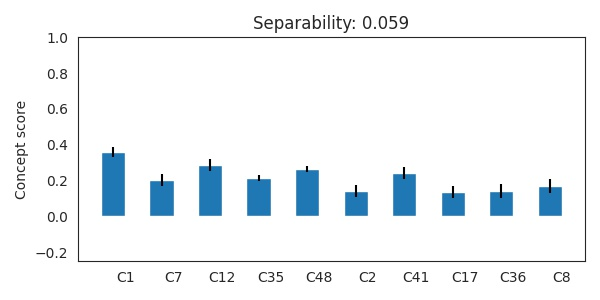
\includegraphics[width=0.45\columnwidth]{yeh_class17_AwA2_top10_detected_Energy.jpg}}
\hfill \hspace{-2mm}
\subfloat[Set 2 with high concept separability, detected-ID \label{fig:high_in}] {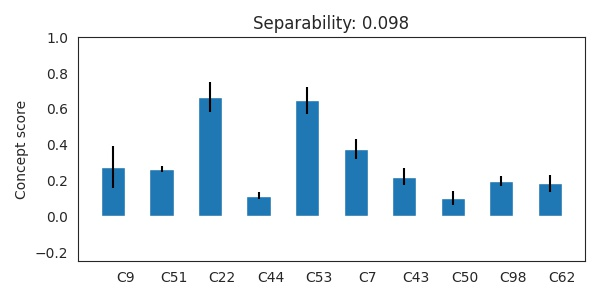
\includegraphics[width=0.45\columnwidth]{figures/ours_class17_AwA2_top10_detected_Energy.jpg}}\hfill\\
% \vspace{-1mm}
\subfloat[Set 1 with low concept separability, detected-OOD \label{fig:low_out}]{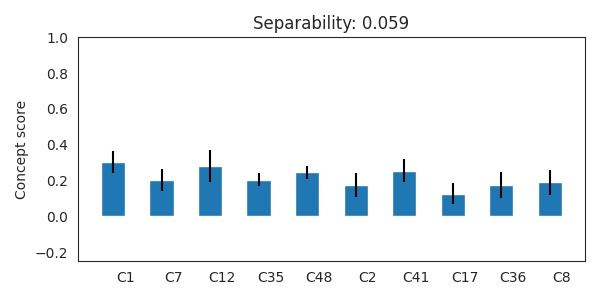
\includegraphics[width=0.45\columnwidth]{figures/yeh_class17_SUN_top10_detected_Energy.jpg}}\hfill
\subfloat[Set 2 with high concept separability, detected-OOD \label{fig:high_out}] {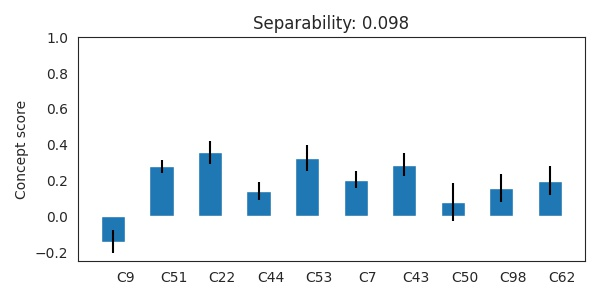
\includegraphics[width=0.45\columnwidth]{figures/ours_class17_SUN_top10_detected_Energy.jpg}}
\caption{
\small \textbf{Our concept separability metric and visual distinction in the concept score patterns.} For the class "Giraffe", we compare the concept score patterns using two different sets of concepts. \textbf{Left:} Averaged concept scores using concept set 1 (top-10 important concepts out of the concepts learned with $\,\lambda_\textrm{mse} = \lambda_\textrm{norm} = \lambda_\textrm{sep} = 0$). 
\textbf{Right:} Averaged concept scores using concept set 2 (top-10 important concepts out of the concepts learned with $\,\lambda_\textrm{mse} = 1, \lambda_\textrm{norm} = 0.1, \lambda_\textrm{sep} = 50$).
Concept importance is measured using the Shapley value of Eqn. (\ref{equ: ConceptSHAP}).
Concept separability is measured based on the presented 10 concepts from each set.
% For visualization of what each concept represents, see Appendix.
% C$i$ denotes $i$-th concept.
}
\label{fig:high_separa_interpretatbility}
\vspace{-0.10in}
% \vspace{-4mm}
\end{figure}

\fi

% Lastly, we illustrate how the concepts learned by our algorithm can be used to provide explanations for an OOD detector.
% By quantifying the contribution of each concept toward OOD detection results, we can identify the major concepts that an OOD detector relies on to make decisions. 
% \begin{itemize}
%     \item What set of the concepts is most prominent across the data detected as ID (or OOD) by $\mathcal{D}$?
%     \item What set of the concepts contribute to distinguish the ID and OOD data detected by $\mathcal{D}$?
%     \item How the change in concept score affects the $\mathcal{D}$'s detection result?
%     % \jihye{check perturbation generation in ATOM <-- permutation in concept space?}
% \end{itemize}
%

\iffalse

\begin{figure}[tb]
\vspace{-5mm}
% \begin{center}
%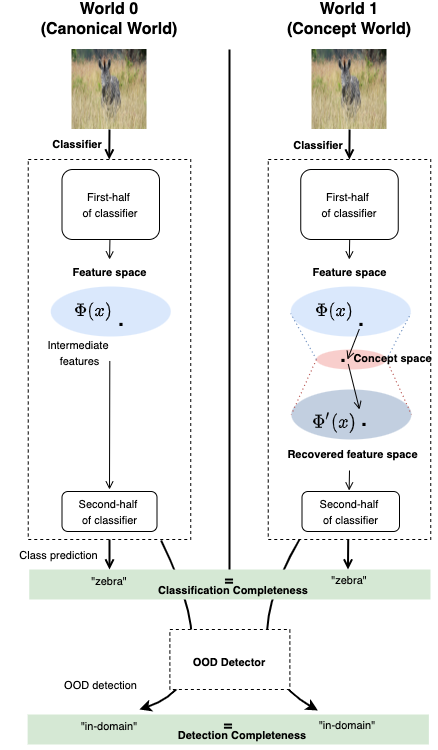
\includegraphics[width=0.45\textwidth]{figures/completeness.png}
% \hspace*{+.5cm} 
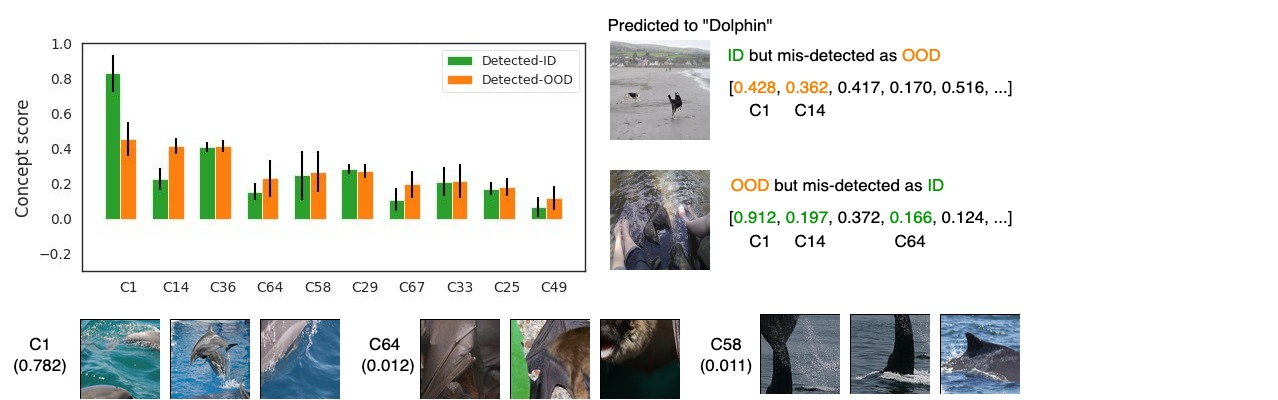
\includegraphics[scale=0.35]{figures/expl_dolphin.png}
% \vspace{-9mm}
\caption{
\small \textbf{Our concept-based explanations for Energy detector given AwA (ID) and SUN (OOD) inputs.} Concepts are discovered by our method with $\lambda_\textrm{mse} = 1, \lambda_\textrm{norm} = 0.1, \lambda_\textrm{sep} = 10$.
Visualized examples for each concept (with the corresponding $\textrm{SHAP}(\eta^{j}_{\bff, S}, 
    \bfc_i)$ score inside the parenthesis) are the receptive fields from $\Dinte$ with highest correlation to the corresponding concept vector $\bfc_i$ where $\langle \bfphi^{p,q}(\bfx), \bfc_i \rangle > 0.85$.
\vspace{-5mm}
}
\label{fig:expl_dolphin}
% \end{center}
\end{figure}

\fi

\iffalse
\begin{figure*}[t]
% \vspace{-3mm}
\centering
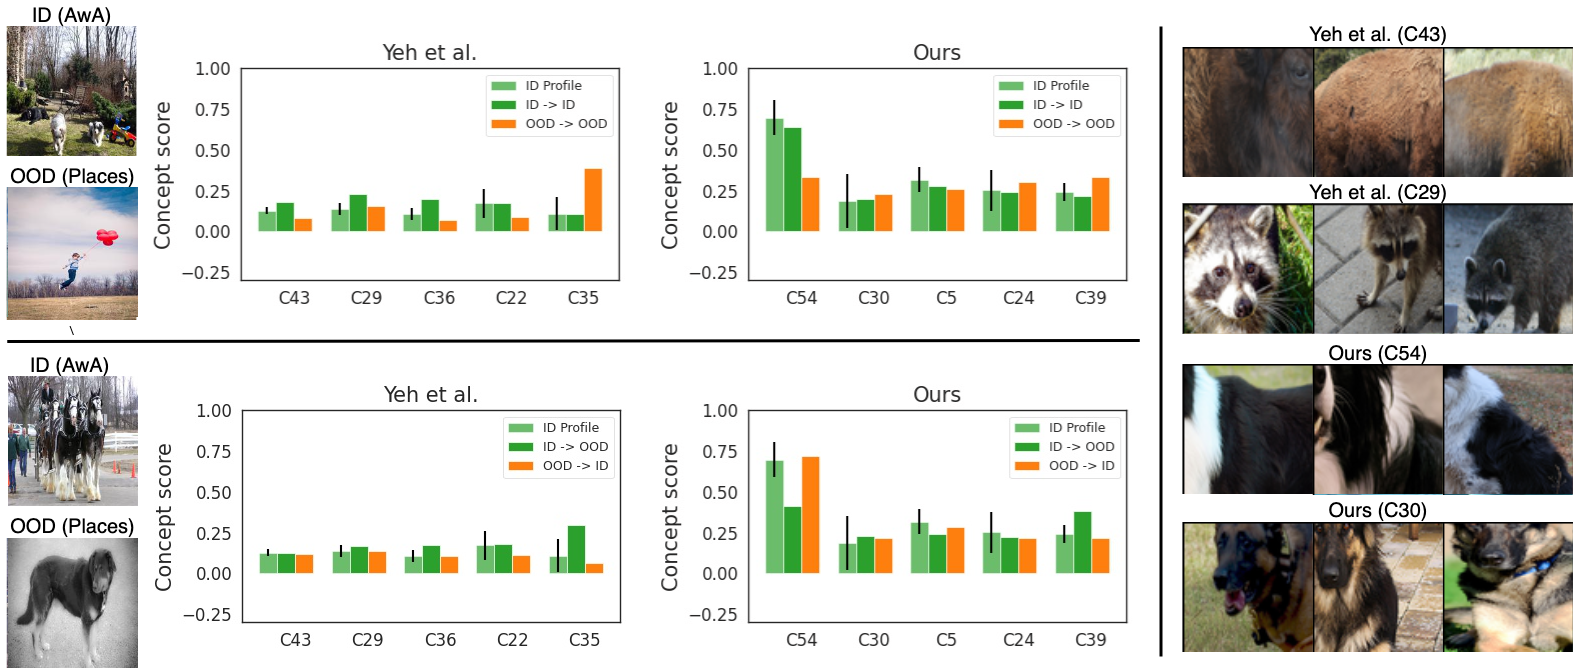
\includegraphics[width=0.9\textwidth]{figures/energy-collie.png}
\caption{\small \textbf{Concept-based explanations for the Energy OOD detector using concepts learned by \citet{yeh2020completeness} vs. ours ($\lambda_\textrm{mse} = 1, \lambda_\textrm{norm} = 0.1, \lambda_\textrm{sep} = 10$)}. Images are randomly selected from the AwA test set (ID) and \texttt{Places} (OOD), and all of them are predicted to the class ``Collie''.
The ID profile (light-green bar) shows the average concept-score pattern for ID images predicted as ``Collie''. 
The top two images correspond to correct detection, \ie ID detected as ID (dark-green bar) and OOD detected as OOD (orange bar).
Similarly, the bottom  two images correspond to incorrect detection.
The right sub-figure illustrates the top two concepts for the method of \citet{yeh2020completeness} and our method.
}
\label{fig:expl-energy-collie}
\vspace{-3mm}
\end{figure*}
\fi




\subsection{Concept-Based Explanations for OOD Detectors}
\label{sec:expt_concept_based_explanations}
% \mypara{Contribution of each concept to detection.}

\mypara{Finding the Key Concepts.}
Given a set of learned concepts, we address the question: {\em how much does each concept contribute to the detection results for inputs predicted to a particular class?}
To address this, we follow recent works that have adopted the Shapley value from Game theory literature~\citep{shapley1953value,fujimoto2006axiomatic} for scoring the importance of a feature subset towards the predictions of a model~\citep{chen2018shapley,lundberg2017shapley,sundararajan2020shapley}.
We propose to use our per-class detection completeness metric $\eta^{j}_{\bff, S}(\bfC)\,$ (Eqn. (\ref{equ: completeness-detection-perclass}) in Appendix \ref{sec:appendix-perclass-completeness}) as the characteristic function of the Shapley value. 
The modified Shapley value of a concept $\bfc_i \in \bfC$ with respect to the predicted class $j \in [L]$ is defined as
% \vspace{-3mm}
\begin{align}
    \label{equ: ConceptSHAP}
    \textrm{SHAP}(\eta^{j}_{\bff, S}, \bfc_i) ~:= \!\!\!\sum_{\bfC' \subseteq \bfC \setminus \{\bfc_i\}} \!\!\! \frac{ \eta^{j}_{\bff, S}\big( \bfC' \cup \{\bfc_i\} \big) ~-~ \eta^{j}_{\bff, S}(\bfC') }{ m\, \binom{m \,-\, 1}{|\bfC'|} },
\end{align}
where $\bfC'$ is a subset of $\bfC$ excluding concept $\bfc_i$.
% A high Shapley value represents the average marginal contribution of $\bfc_i$ across all possible coalitions with all classes considered.
This Shapley importance score captures the average marginal contribution of concept $\bfc_i$ towards explaining the decisions of the OOD detector for inputs predicted into class $j$.
% To do so, we simply modify our detection completeness definition (Def. (\ref{def:completeness_detec})) into a per-class variant by considering data predicted into a specific class $j$.
% Also, $b_r = 0.5$ is the AUROC of a random detector.
% Note that for numerator we use predicted label -- don't have labels for OOD data. 
% Accordingly, we use SHAP($\eta^{j}_{\bff, S}(\bfC)$) to denote the Shapley score specific to class $j$.
% where $\eta^{}_{\bff, S}(\bfC)$ is replaced in Eqn. (\ref{equ: completeness-detection-perclass}).

In the rest of the section, we demonstrate how the concepts ranked by the above Shapley importance score can serve as a useful tool for interpreting the OOD detector.


\mypara{Explaining Detection Errors.}
% Eventually, we interpret the behavior of the given OOD detector by plotting the concept score patterns with respect to the concepts ranked by the above Shapley importance score.
Given an OOD detector of interest, we collect inputs that are correctly detected as ID, and average their concept scores (which corresponds to the \textit{ID profile} in Fig.~\ref{fig:expl-energy-collie}).
The ID profile quantifies how much each concept matters for the normal ID inputs.
Given a test input, either correctly or incorrectly detected, the user could examine how similar or different this input is with respect to the ID concept profile.
Fig.~\ref{fig:expl-energy-collie} illustrates our explanations of the Energy OOD detector's decisions.
By visualizing the concepts (see Fig.~\ref{fig:collie-concepts}), we observe that for the predicted class \textit{Collie}, ``furry dog skin'' (C54) and ``oval dog face'' (C30) are the key concepts to capture the detector's outputs to distinguish ID images from OOD images.
% given correctly-detected inputs (ID\,/\,OOD input detected as ID\,/\,OOD; first row of figure), and incorrectly-detected inputs (ID\,/\,OOD input detected as OOD\,/\,ID; second row of figure).
We also observe that the OOD detector predicts an input as ID when the concept scores show a similar pattern to the ID profile, or predicts an input as OOD when the concept-score pattern is far from the ID profile.
For instance, our analysis shows that the bottom input in Fig.~\ref{fig:collie-wrong} is an OOD image from \texttt{Places} dataset but detected as ID (false positive) since its score for ``furry dog skin'' is as high as the usual ID Collie images (which is true in the image). 
Explaining detection results is crucial for encouraging the adoption of OOD detectors in various decision-making processes.
Our example here suggests that certain errors of an OOD detector can be understandable mistakes, which require further reasoning, rather than discarding the model based only on aggregate performance  metrics.
% Thus, we conclude this to be an understandable mistake by the OOD detector.
Additional examples of our concept-based explanations are given in Appendix~\ref{app:more-expl}.

\mypara{Comparison of Explanations by~\citeauthor{yeh2020completeness} and Ours.}
Lastly, we provide qualitative evidence supporting our argument that: concepts good for the classifier are not necessarily good for the OOD detector.
In Fig.~\ref{fig:expl-energy-collie}, given an Energy detector and ID/OOD inputs, we present explanations using  concepts learned by \citet{yeh2020completeness} vs. our method.
We observe that~\citet{yeh2020completeness} fails to generate visually-distinguishable explanations between detected-ID and detected-OOD inputs.
The separation between the dark-green bars and the orange bars in Fig.~\ref{fig:collie-correct} and Fig.~\ref{fig:collie-wrong} becomes more visible in our explanations, which enables more intuitive interpretation for human users (this reflects our design goal of concept separability).
It is also noteworthy that in Fig.~\ref{fig:collie-concepts}, our concepts that are most important to distinguish ID Collie from OOD Collie (\ie C54 and C30) are more specific and finer-grained characteristics of Collie, while \citet{yeh2020completeness} finds concepts that are vaguely similar to the features of a dog, but rather generic (\ie C43 and C29).
This is the reason we require more number of concepts to achieve high detection completeness and concept separability, compared to solely considering the classification completeness~\footnote{In Fig.~\ref{fig:expl-energy-collie}, after concept learning with $m = 100$ and duplicate removal, we found 44 non-redundant concepts for ~\citet{yeh2020completeness}, and 100 distinct concepts for ours.}.
% \jihye{@others: may add one more closing/concluding statement?}


% \subsection{Bootstrapping explanations for better OOD detection}
\subsection{Explanations For Better OOD Detection.}
Our work makes the first effort to reason about the different failure modes of OOD detectors through explanations, rather than just observing aggregated performance metrics (e.g., AUROC or AUPRC).
Naturally, the next step would be to utilize such reasoning to modify and improve the OOD detector. 
% While leaving the development of concept-based explanations as actionable guidelines for better OOD detection as a future work, here we provide a scenario where our explanations can provide direct utility.
We leave the development of concept-based explanations as actionable guidelines for better OOD detection as future work, and describe here a scenario where our explanations can provide direct utility.

We posit that our explanations can provide effective feedback when the failure of the OOD detector originates from misbehavior of the paired classifier, which we confirm to be the most common failure mode of OOD detectors. 
For instance, consider the top image in Fig.~\ref{fig:collie-wrong} as our input. Its true label is ``Horse'', but the classifier predicted it to class ``Collie''. Obviously, the horse image has a different concept-activation pattern from the normal ID Collie profile (compare the dark-green bars with the ID profile of ours in Fig.~\ref{fig:collie-wrong}). 
To remove such failure cases, the practitioner could identify the key concepts for the prediction of class ``Horse'' and compare the concept pattern of the input to the normal ID ``Horse'' profile. It is noteworthy that we can use the same set of concepts here, since our concept-learning objective finds concepts that can effectively explain \textit{both} the classifier and OOD detector. Indeed, we observe that the key concepts for the class ``Horse'' are ``round brown body'' and ``brown oval face of horse'', while the given input is an outlier relative to these concepts. 
Hence, the practitioner could consider diversifying the training set in the ID ``Horse'' class to include more examples of horses (\eg with black and white hair).

\iffalse

Based on this concept importance metric, we can interpret the misbehavior of the given OOD detector.
Fig. \ref{fig:expl_dolphin} shows the averaged concept scores of top-10 important concepts for Energy detector between correctly detected-ID and -OOD inputs that are predicted to class ''Dolphin'' (namely, correct profiles).
Given a random ID input that is mis-detected into OOD by the OOD detector, we observe that its concept scores rather follow the detected-OOD profiles (or vice-versa, for OOD input mis-detected into ID); specifically, unusually low score for C1 (blue, wavy surface of the sea) and high score for C14~\footnote{We could not visualize C14 as there is no receptive fields with correlation to $\bfc_{14}$ greater than $0.85$, which confirms the trade-off between concept separability and human understandability, as discussed in Appendix \ref{sec:appendix-concept-learning-ablation}}, and it would look reasonable for the OOD detector to think the ID input with such OOD-like characteristics to be OOD. 
Such inspection of the OOD detector's mistakes could assist the practitioner in examining whether it was a reasonable mistake even for humans, or whether the OOD detector is simply unreliable. See Appendix \ref{sec:appendix-shapleys} for more examples of explanations.

More examples can be found in Appendix.
we present the top-ranked concepts along with the visualized examples that are nearest to the corresponding concept vector in Fig. \ref{fig:shap_buffalo}.
For the baseline method \citep{yeh2020completeness} (denoted ``baseline'' in Fig. \ref{fig:shap_buffalo}), the learned concepts are solely intended for reconstructing the behavior of the classifier. 
In this case, we observe from Fig. \ref{fig:shap_buffalo} that 
% a common set of concepts (\ie concepts 32, 10, and 47) are selected for interpreting both the classifier and OOD detector.
interpretation of both the classifier and OOD detector depends on a common set of concepts (\ie concepts 32, 10, and 47).
On the other hand, the concepts learned by our method focus on reconstructing the behavior of both the OOD detector and the classifier. In this case, we observe from Fig. \ref{fig:shap_buffalo} that a distinct set of important concepts are selected for classification and OOD detection.
We also observe that our method requires more concepts in order to address the decisions of both the classifier and OOD detector.
For instance, the number of concepts obtained by our method and the baseline are 78 and 53 (respectively), out of a total 100 concepts~\footnote{After removing redundant concepts for which the inner-product between the corresponding concept vector and any of the remaining concept vectors is larger than $0.95$.}.
More examples of concepts with high-ranking Shapley scores can be found in Appendix \ref{sec:appendix-explanation}.
We further investigate the attribution of such top-ranked concepts via counterfactual analysis in Appendix \ref{sec:appendix-counterfactual}.

\fi

% \mypara{Separability and interpretatbility}
% \begin{figure*}
%   \centering
%   \begin{tabular}{cc}
%     \subfloat[\label{fig:mnist}][Sampling distribution is skewed consistently for a single class (i.e. class 0)]
%     {
%     \hspace{-5mm}
%     \includegraphics[width=.49\linewidth]{mnist_class_0}} 
%     ~&~
%     \subfloat[\label{fig:asd}][Sampling distribution is skewed for the classes in turn (i.e. class 0, 1, 2, ...)]
%     {\includegraphics[width=.49\linewidth]{mnist_class_all}}
%   \end{tabular}
%   \caption{Accuracy vs training time-step in MNIST}
% \label{fig:mnist_results}
% \end{figure*}


% \section{Related Work}
\mypara{OOD detection.}
Starting with a simple baseline for OOD detection based on the maximum softmax probability (MSP) score \cite{hendrycks2016msp}, recent studies have designed various scoring functions based on the outputs from the final or penultimate layers \cite{liang2018ODIN, devries2018learning}, or a combination of different intermediate layers of DNN model \cite{lee2018mahalanobis}.
Our general framework can be applied to these existing OOD detection methods by choosing a suitable intermediate layer for concept-based interpretation~\footnote{For instance, if an OOD detector makes decisions based on outputs from an intermediate layer $\ell$, the user can explain it using concepts that can reconstruct the feature representations from layer $\ell$, or an earlier layer.}.
To further improve the OOD uncertainty estimation, several works attempt to finetune the DNN classifier using auxiliary OOD training data \cite{hendrycks2018OE,lee2018training,chen2021atom}.
Complementary to these, our work is a post-hoc method that aims to explain an already-trained DNN model and its paired OOD detector. 
Our concept learning algorithm discovers concepts through optimization based on the feature representations from a DNN layer, without modifying the internals of the DNN or the OOD detector. \jihye{details of OOD to appendix}

\mypara{Post-hoc interpretability.}
Feature attribution is the most commonly used post-hoc explanation method that attributes the decision to local input features~\cite{baehrens2009grad, simonyan2013grad, smilkov2017smoothgrad, sundararajan2017IG}, but recent works have demonstrated its vulnerability to \eg adversarial perturbations~\cite{ghorbani2019fragile,heo2019fooling,slack2020fooling}. 
Adebayo \etal~\cite{adebayo2020debugging} also conduct experimental analyses and a human subject study to assess the effectiveness of feature attributions under various settings (including on OOD data), and show that feature attributions barely have any visual difference between ID inputs and OOD inputs.
% Through human subject study, they also illustrate that users do not find the resulting explanations to be intuitive guidance deciding whether to trust model predictions with OOD inputs. 

On the other hand, concept-based explanation is another type of interpretation method, which is designed to be better-aligned with human reasoning \cite{armstrong1983human-concepts,tenenbaum1999concept-learning} and intuition~\cite{ghorbani2019ace,zhou2018interpretable,bouchacourt2019educe,yeh2020completeness}. 
% Motivated by that human reasoning follows concept-based thinking by grouping similar examples and identifying resembled patterns across them \cite{armstrong1983human-concepts,tenenbaum1999concept-learning}, a line of works aimed to reason about model behaviors in a similar way as human thinking so that the resulting explanations would be more intuitive to humans \cite{kim2018tcav,ghorbani2019ace,zhou2018interpretable,bouchacourt2019educe}. 
A common implicit assumption in the concept-based explanation literature is {\em linear interpretability}, \ie the concepts lie in a linearly-projected subspace of intermediate DNN layer activations; our work is also based on this assumption.
While the scope of existing works is confined to explaining DNN classifiers, we extend the use of concept-based interpretability for explaining OOD detectors.
Our work is inspired by \cite{yeh2020completeness}, and we extend their concept-based explanation method for DNN classifiers to OOD detectors. As discussed in section \ref{sec:concept_learning}, the concept learning objective of \cite{yeh2020completeness} can be obtained as a special case of our concept learning objective for the hyper-parameter setting $\,\lambda_{\textrm{norm}} = \lambda_{\textrm{mse}} = \lambda_{\textrm{sep}} = 0$.


\iffalse

The most commonly used post-hoc explanation for DNN prediction is feature attribution, which attributes the decision to local input features \cite{baehrens2009grad, simonyan2013grad, smilkov2017smoothgrad, sundararajan2017IG}. 
% Notwithstanding the wide adoption of feature attribution to various applications \cite{}, 
Recent works have demonstrated that feature attributions are vulnerable \cite{ghorbani2019fragile,heo2019fooling,slack2020fooling}. 
\citeauthor{adebayo2020debugging} also conducts experimental analysis and human subject study to assess the effectiveness of feature attributions under various settings including OOD data, and show that feature attributions barely have visual difference between ID inputs and OOD inputs.

On the other hand, concept-based explanation is another type of interpretability to globally explain how DNN model reasons.
Motivated by that human reasoning follows concept-based thinking by grouping similar examples and identifying resembled patterns across them \cite{armstrong1983human-concepts,tenenbaum1999concept-learning}, a line of works aimed to reason about model behaviors in a similar way as human thinking so that the resulting explanations would be more intuitive to humans \cite{kim2018tcav,ghorbani2019ace,zhou2018interpretable,bouchacourt2019educe}. 
A common implicit assumption in concept-based explanation literature is linear interpretability: concepts lie in the linearly projected space of intermediate DNN activations, and our work is also based on this assumption.
Yet, while the scope of existing works is only focused on only explaining DNN prediction, we extend the use of concept-based interpretability to reasoning OOD detectors.

\fi



\iffalse
There is a growing need for post-hoc explanation methods that can be applied to working high performance DNN models that are deployed to the real-world without taking interpretability into consideration during training.
Recent studies have focused on assessing the effectiveness of post-hoc explanations ranging from human-centric evaluations [2, 5] to functionally-grounded evaluations [19, 20, 21, 22, 10, 23].
Our work is in line with contributions of evaluation of explanations; albeit with an emphasis on interpreting OOD detectors.

Contrary to the great interest in achieving high OOD detection performance, there is little effort to develop methods that can effectively reason about the detection decisions.
\cite{adebayo2020debugging} suggests caution for using feature attributions \cite{baehrens2009grad, simonyan2013grad, smilkov2017smoothgrad, sundararajan2017IG} to inspect ID and OOD inputs through empirical assessment and human subject tests.
As such, our concentration is on developing a method based on human-friendly concepts.

Concept-based explanation is a type of explanation method that .... \cite{kim2018tcav, koh2020concept-bottleneck, ghorbani2019ace}.
This line of works are based on an implicit assumption that the concepts lie in low-dimensional subspaces of some intermediate DNN activations.

concept-based explanations.. regarding the assumptions that concepts \jihye{emphasize why we chose Yeh et al. as baseline of our work, out of other concept-based explanation works -- limitations of them.} \jihye{we show the inappropriateness of concept-based explanation only with \cite{yeh2020completeness}. Need to elaborate why we chose Yeh et al. as baseline of our work out of other concept-based explanation works.} \\.\\.\\our method is also post-hoc.\\. 

The gold standard for assessing the effectiveness of an explanation is a human subject study (DoshiVelez and Kim, 2017). Poursabzi-Sangdeh et al. (2018) 
\fi





% \mypara{Interaction-centric explanations for OOD detection.}
% \jihye{should we briefly reveal our plan for the followup work? or not necessary?}

\section{Conclusion}
We develop an unsupervised and human-interpretable explanation method for black-box OOD detectors based on high-level concepts derived from the internal layer representations of a (paired) DNN classifier.
% In this work, we make a first attempt at developing an unsupervised and human-interpretable explanation method for black-box OOD detectors based on high-level concepts derived from an internal layer representation of a (paired) DNN classifier.
We propose novel metrics viz. {\em detection completeness} and {\em concept separability} to evaluate the completeness (sufficiency) and quality of the learned concepts for OOD detection.
We then propose a concept learning method that is quite general and applies to a broad class of off-the-shelf OOD detectors.
Through extensive experiments and qualitative examples, we demonstrate the practical utility of our method for understanding and debugging OOD detectors.
We discuss additional aspects of our method such as the auxiliary OOD dataset, human subject study, and societal impact in Appendix~\ref{sec:app_discussion}.

\iffalse

This work introduces a first method (to the best of our knowledge) for providing concept-based attributions of the decision of an OOD detector based on high-level concepts derived from the internal layer representations of a (paired) DNN classifier.
% We define the concept evaluation criteria of detection completeness and concept separability and propose a general framework for learning concepts that satisfy the criteria without involving laborious human effort for concept annotations.
By treating OOD detectors as a black-box, our framework applies to a wide variety of OOD detectors.
%Our general framework can be applied to these existing OOD detection methods by choosing a suitable intermediate layer for concept-based interpretation~\footnote{For instance, if an OOD detector makes decisions based on outputs from an intermediate layer $\ell$, the user can explain it using concepts that can reconstruct the feature representations from layer $\ell$, or an earlier layer.}.

\mypara{Auxiliary OOD Dataset.} 
%Our approach also remains a limitation in that an auxiliary dataset of an OOD distribution is required.
A limitation of our approach is its requirement of an auxiliary OOD dataset for concept learning, which could be hard to access in certain applications.
% A weakness of our approach is that it requires an auxiliary OOD dataset for concept learning. 
% Unfortunately, access to such data could be a luxury in certain applications.
To overcome that, a research direction would be to design generative models that simulate domain shifts or anomalous behavior and could create the auxiliary OOD dataset synthetically, allowing us additional control on the extent of distributional changes the resulting concepts could deal with (see Appendix~\ref{app:auxiliary-ood} for further discussion). 

% We believe this work takes a step toward building trust in the deployment of OOD detectors, which will help the practical integration of such systems towards making societal decisions.

\mypara{Human Subject Study.} 
% One would suggest performing a user study to get a more extensive understanding of the effectiveness of our method in the hands of ML practitioners.
Performing a human-subject (or user) study would be the ultimate way to evaluate the effectiveness of explanations, but remains largely unexplored even for in-distribution classification tasks.  
We emphasize that designing such a usability test with OOD detectors would be even more challenging due to the characteristics of the OOD detection task, compared to in-indistribution classification tasks.
For in-distribution classifiers, users could potentially generate hypotheses about what high-level concepts should attribute to the class prediction, and compare their hypotheses to the provided explanations to determine the classifier's reliability.
On the other hand, assessing the reliability of OOD detection involves checking whether a given input belongs to any of the natural distributions of concepts; this is essentially limited to whether users' mental models on such global distributions can be accurately probed via a couple of presented local instances.
We believe that designing a thorough probing method for human interpretability on OOD detection would be an interesting yet challenging research quest by itself and our paper does not address that.

\mypara{Societal Impact.}
\label{sec:broader_impact}
Our work helps address the detection results of OOD detectors, giving practitioners the ability to explain the model's decision to invested parties. 
Our explanations can also be used to keep a data point as an understood mistake by the model rather than throwing it away without further analysis, which could help guide how to improve the OOD detector with respect to the concepts. 
However, this would also mean that more trust is put back into the human practitioner to not abuse the explanations or misrepresent them. 


% (\eg feature attribution).
% such as feature attribution or concept-based interpretability for class predictions.

% Future work -- what to do with such explanations on ood detections. What kind of help to ml practitioners? \\.\\.
% usefulness of concept-based explanation vs feature attribution method for OOD detection explanations -- conduct human-centric evaluations
% This paper takes a step toward interpreting what makes data to be detected as in-distribution or OOD, and what are the distinguishing characteristics between in-distribution and OOD data.
% malicious distribution shift

In this work, we propose a first method (to the best of our knowledge) for providing concept-based attributions of the decisions of an OOD detector based on high-level concepts derived from the internal feature representations of a DNN classifier.
We quantify how a set of concepts can  accurately describe an OOD detector's behavior through our detection completeness metrics. 
We also propose a general framework for learning concepts, that does not involve human-based concept annotations, by incorporating regularization terms that ensure accurate reconstruction of the feature representation space based on concept scores.
% In future work, one could reduce the performance gap of the DNN classifier and OOD detector even further in our two-world view by bringing insights from the knowledge-distillation literature to the regularization design \cite{romero2014fitnets, zagoruyko2016paying}.
% In addition to detection completeness, we propose a concept separability metric that can be directly plugged into our concept learning framework. 
Our explanations with diverse OOD detectors and datasets confirm our insight that separability in the concept space leads to better distinction between the resulting explanations for ID and OOD-detected inputs.
% , hence bringing more intuitive interpretations. 
Future work includes human-centric evaluations \cite{doshi2017towards, poursabzi2021manipulating} to assess how real users find our concept-based explanations compared to explanations generated by prior works.

\fi


% Acknowledgements should only appear in the accepted version.
\section*{Acknowledgements}
We thank all the anonymous reviewers for their careful comments and feedback.
The work is partially supported by Air Force Grant FA9550-18-1-0166, the National Science Foundation (NSF) Grants CCF-FMitF-1836978, IIS-2008559, SaTC-Frontiers-1804648, CCF-2046710, CCF-1652140, and 2039445, and ARO grant number W911NF-17-1-0405. Choi, Feng, Chen, Jha, and Prakash are partially supported by the DARPA-GARD problem under agreement number 885000.
Raghuram is partially supported through the NSF grants CNS-2112562, CNS-2107060, CNS-2003129, CNS-1838733, CNS-1647152, and the US Department of Commerce grant 70NANB21H043.

\bibliographystyle{icml2023}
\bibliography{references}

% \section*{Checklist}

\iffalse
%%% BEGIN INSTRUCTIONS %%%
The checklist follows the references.  Please
read the checklist guidelines carefully for information on how to answer these
questions.  For each question, change the default \answerTODO{} to \answerYes{},
\answerNo{}, or \answerNA{}.  You are strongly encouraged to include a {\bf
justification to your answer}, either by referencing the appropriate section of
your paper or providing a brief inline description.  For example:
\begin{itemize}
  \item Did you include the license to the code and datasets? \answerYes{See Section~\ref{gen_inst}.}
  \item Did you include the license to the code and datasets? \answerNo{The code and the data are proprietary.}
  \item Did you include the license to the code and datasets? \answerNA{}
\end{itemize}
Please do not modify the questions and only use the provided macros for your
answers.  Note that the Checklist section does not count towards the page
limit.  In your paper, please delete this instructions block and only keep the
Checklist section heading above along with the questions/answers below.
%%% END INSTRUCTIONS %%%
\fi

\begin{enumerate}


\item For all authors...
\begin{enumerate}
  \item Do the main claims made in the abstract and introduction accurately reflect the paper's contributions and scope?
    \answerYes{}
  \item Did you describe the limitations of your work?
    \answerYes{}
  \item Did you discuss any potential negative societal impacts of your work?
    \answerYes{See Section \ref{sec:broader_impact}}
  \item Have you read the ethics review guidelines and ensured that your paper conforms to them?
    \answerYes{}
\end{enumerate}


\item If you are including theoretical results...
\begin{enumerate}
  \item Did you state the full set of assumptions of all theoretical results?
    \answerNA{}
        \item Did you include complete proofs of all theoretical results?
    \answerNA{}
\end{enumerate}


\item If you ran experiments...
\begin{enumerate}
  \item Did you include the code, data, and instructions needed to reproduce the main experimental results (either in the supplemental material or as a URL)?
    \answerYes{}
  \item Did you specify all the training details (e.g., data splits, hyperparameters, how they were chosen)?
    \answerYes{See Section \ref{sec:setup}}
        \item Did you report error bars (e.g., with respect to the random seed after running experiments multiple times)?
    \answerYes{See Table \ref{tab:concept-learning-results}}
        \item Did you include the total amount of compute and the type of resources used (e.g., type of GPUs, internal cluster, or cloud provider)?
    \answerYes{See Appendix \ref{sec:appendix-implementation-details}}
\end{enumerate}


\item If you are using existing assets (e.g., code, data, models) or curating/releasing new assets...
\begin{enumerate}
  \item If your work uses existing assets, did you cite the creators?
   \answerYes{See References}
  \item Did you mention the license of the assets?
    \answerNA{}
  \item Did you include any new assets either in the supplemental material or as a URL?
    \answerNA{}
  \item Did you discuss whether and how consent was obtained from people whose data you're using/curating?
    \answerNA{}
  \item Did you discuss whether the data you are using/curating contains personally identifiable information or offensive content?
    \answerNA{}
\end{enumerate}


\item If you used crowdsourcing or conducted research with human subjects...
\begin{enumerate}
  \item Did you include the full text of instructions given to participants and screenshots, if applicable?
    \answerNA{}
  \item Did you describe any potential participant risks, with links to Institutional Review Board (IRB) approvals, if applicable?
   \answerNA{}
  \item Did you include the estimated hourly wage paid to participants and the total amount spent on participant compensation?
    \answerNA{}
\end{enumerate}


\end{enumerate}
\newpage
\appendix
\onecolumn
\begin{center}
	\textbf{\LARGE Appendix }
\end{center}

% \begin{center}
% 	\textbf{\large Concept-based Explanations for Out-of-Distribution Detectors}
% \end{center}
In Section~\ref{sec:app_discussion}, we discuss additional aspects of our method such as the choice of auxiliary OOD dataset, human subject study, and societal impact.
In Section \ref{sec:appendix-A}, we discuss the connection of the proposed concept separability to Bhattacharya Distance, and the per-class variations of detection completeness and concept separability, followed by the overall algorithm for concept learning.
In Section \ref{sec:appendix-implementation-details}, we provide the detailed setup for the experiments and additional thorough analysis of our concept learning objective.
In Section \ref{app:auxiliary-ood}, we discuss whether our concept learning objective remains effective even when a synthesized auxiliary OOD dataset similar to target ID data is used.
In Section \ref{sec:appendix-shapleys}, we illustrate additional examples of our concept-based explanations.


% short analysis of the ConceptSHAP in the appendix like Yeh et al do
% Connection to dimensionality reduction, Fisher's score?
\section{Discussion and Societal Impact}
\label{sec:app_discussion}
\mypara{Auxiliary OOD Dataset.} 
%Our approach also remains a limitation in that an auxiliary dataset of an OOD distribution is required.
A limitation of our approach is its requirement of an auxiliary OOD dataset for concept learning, which could be hard to access in certain applications.
% A weakness of our approach is that it requires an auxiliary OOD dataset for concept learning. 
% Unfortunately, access to such data could be a luxury in certain applications.
To overcome that, a research direction would be to design generative models that simulate domain shifts or anomalous behavior and could create the auxiliary OOD dataset synthetically, allowing us additional control on the extent of distributional changes the resulting concepts could deal with (see Appendix~\ref{app:auxiliary-ood} for further discussion). 

% We believe this work takes a step toward building trust in the deployment of OOD detectors, which will help the practical integration of such systems towards making societal decisions.

\mypara{Human Subject Study.} 
% One would suggest performing a user study to get a more extensive understanding of the effectiveness of our method in the hands of ML practitioners.
Performing a human-subject (or user) study would be the ultimate way to evaluate the effectiveness of explanations, but remains largely unexplored even for in-distribution classification tasks.  
We emphasize that designing such a usability test with OOD detectors would be even more challenging due to the characteristics of the OOD detection task, compared to in-indistribution classification tasks.
For in-distribution classifiers, users could potentially generate hypotheses about what high-level concepts should attribute to the class prediction, and compare their hypotheses to the provided explanations to determine the classifier's reliability.
On the other hand, assessing the reliability of OOD detection involves checking whether a given input belongs to any of the natural distributions of concepts; this is essentially limited to whether users' mental models on such global distributions can be accurately probed via a couple of presented local instances.
We believe that designing a thorough probing method for human interpretability on OOD detection would be an interesting yet challenging research quest by itself~\cite{kim2022hive} and our paper does not address that.

\mypara{Societal Impact.}
\label{sec:broader_impact}
Our work helps address the detection results of OOD detectors, giving practitioners the ability to explain the model's decision to invested parties. 
Our explanations can also be used to keep a data point as an understood mistake by the model rather than throwing it away without further analysis, which could help guide how to improve the OOD detector with respect to the concepts. 
However, this would also mean that more trust is put back into the human practitioner to not abuse the explanations or misrepresent them. 

\section{Concept Learning}
\label{sec:appendix-A}
\subsection{Connection to the Bhattacharya Distance}
\label{sec:appendix-BC-distance}
We note that the proposed separability metric in Section \ref{sec:separability_score} is closely related to the Bhattacharya distance~\cite{bhattacharyya1943measure} for the special case when the concept scores from both ID and OOD data follow a multivariate Gaussian density. The Bhattacharya distance is a well known measure of divergence between two probability distributions, and it has the nice property of being an upper bound to the Bayes error rate in the two-class case~\cite{fukunaga1990bhatta}. For the special case when the concept scores from both ID and OOD data follow a multivariate Gaussian with a shared covariance matrix, it can be shown that the Bhattacharya distance reduces to the following separability metric (ignoring scale factors): 
\begin{align}
\label{eq:separability_trace}
&J_{\textrm{sep}}(\bfC) ~:=~ J_{\textrm{sep}}(V_{\textrm{in}}(\bfC), V_{\textrm{out}}(\bfC)) ~=~ \textrm{tr}\big[\bfS_w^{-1} \,\bfS_b\big].
%
% &=~ \textrm{tr}\big[\bfS_w^{-1} \,(\bfmu_{\textrm{out}} \,-\, \bfmu_{\textrm{in}})\,(\bfmu_{\textrm{out}} \,-\, \bfmu_{\textrm{in}})^T\big] \nonumber \\
%
% &=~ (\bfmu_{\textrm{out}} \,-\, \bfmu_{\textrm{in}})^T \,\bfS_w^{-1} \,(\bfmu_{\textrm{out}} \,-\, \bfmu_{\textrm{in}}).
\end{align}

\iffalse

We sometimes denote $J_{\textrm{sep}}(V_{\textrm{in}}(\bfC), V_{\textrm{out}}(\bfC))$ as $J_{\textrm{sep}}(\bfC)$ for brevity.
Assumption of unimodal distribution; when this assumption may not be appropriate in some cases. 
\fi

\subsection{Per-class Detection Completeness}
\label{sec:appendix-perclass-completeness}
We propose a per-class measure for the detection completeness (denoted by $\eta^{y}_{\bff, S}(\bfC)$), which is obtained by simply modifying $\eta^{}_{\bff, S}(\bfC)$ in Eqn. (\ref{equ: completeness-detection}) based on the subset of ID and OOD data that are predicted into class $y \in [L]$ by the classifier.
% One can simply compute Eqn. (\ref{equ: completeness-detection}) and Eqn. (\ref{eq:separability_trace}) using the subset of ID and OOD data whose predictions are class $y \in [L]$. 
% We refer to this per-class variation as the \textit{per-class detection completeness} (denoted by $\eta^{y}_{\bff, S}(\bfC)$).

\begin{definition}
\label{def:completeness_detec_perclass}
Given a trained DNN classifier $\bff = \bfh \circ \bfphi$, a trained OOD detector with score function $S(\bfx, \bff)$, and a set of concept vectors $\bfC$, the {\em per-class detection completeness} relative to class $y \in [L]$ with respect to the ID distribution $\Pin(\bfx, y)$ and OOD distribution $\Pout(\bfx)$ is defined as
\begin{align}
\label{equ: completeness-detection-perclass}
    \eta^{y}_{\bff, S}(\bfC) 
    ~:=~ \frac{\textrm{sup}_\bfg \,\textrm{AUC}^y(\bfh \circ \recphi) ~-~ b_r}{\textrm{AUC}(\bfh \circ \bfphi) ~-~ b_r},
\end{align}
\end{definition}
where $\textrm{AUC}^y(\bfh \circ \recphi)$ is the AUROC of the detector conditioned on the event that the class predicted by the concept-world classifier $\,\bfh \circ \recphi\,$ is $y$. We note that the denominator in the above metric is still the global AUROC. The baseline AUROC $b_r$ is equal to $0.5$.
This per-class detection completeness is used in the modified Shapley value defined in Section \ref{sec:expt_concept_based_explanations}.

\subsection{Per-class Concept Separability}
\label{sec:appendix-perclass-separability}
In section \ref{sec:separability_score}, we focused on the separability between the concept scores of ID and OOD data without considering the class prediction of the classifier.
However, it would be more appropriate to impose a high separability between the concept scores on a per-class level. In other words, we would like the concept scores of detected-ID and detected-OOD data, that are predicted by the classifier into any given class $y \in [L]$ to be well separated.
Consider the set of concept-score vectors from the detected-ID (or detected-OOD) dataset that are also predicted into class $y$:
\begin{align}
V^{y}_{\textrm{in}}(\bfC) ~&:=~ \{\TVC(\bfx), ~\bfx \in \Dintr \cup \Douttr ~:~ \calD_\gamma(\bfx, \bff) = 1~ \text{ and } ~\widehat{y}(\bfx) = y\} \nonumber \\
%
V^{y}_{\textrm{out}}(\bfC) ~&:=~ \{\TVC(\bfx), ~\bfx \in \Dintr \cup \Douttr ~:~ \calD_\gamma(\bfx, \bff) = 0~ \text{ and } ~\widehat{y}(\bfx) = y\}.
\end{align}
We can extend the definition of the global separability metric in Eq. (\ref{eq:separability_trace}) to a given predicted class $y \in [L]$ as follows
\begin{align}
\label{eq:separability_trace_per_class}
J^y_{\textrm{sep}}(\bfC) ~&:=~ J_{\textrm{sep}}(V^{y}_{\textrm{in}}(\bfC), V^{y}_{\textrm{out}}(\bfC)) ~=~ \textrm{tr}\big[(\bfS^{y}_w)^{-1} \,\bfS^y_b\big] \nonumber \\
&=~ (\bfmu^y_{\textrm{out}} \,-\, \bfmu^y_{\textrm{in}})^T \,(\bfS^y_w)^{-1} \,(\bfmu^y_{\textrm{out}} \,-\, \bfmu^y_{\textrm{in}}).
\end{align}
We refer to these per-class variations as \textit{per-class concept separability}.
The scatter matrices $\bfS^y_w$ and $\bfS^y_b$ are defined similar to Eq. (\ref{eq:scatter_matrices}), using the per-class subset of concept scores $V^{y}_{\textrm{in}}(\bfC)$ or $V^{y}_{\textrm{out}}(\bfC)$, and the mean concept-score vectors from the detected-ID and detected-OOD dataset are also defined at a per-class level.

% Ideally, a high global concept separability would ensure that on a macro level the concepts provide clear explanations regardless of the class and decision of the classifier. But, since the goal is to provide concept explanations for OOD detectors, we could still provide meaningful explanations on a per-class basis if we can separate out concepts that are from an OOD input classified as a certain class $c$, versus an ID input classified as $c$. Examining both metrics can help us gauge the relative separability on finer and coarser scales to evaluate the quality of the concept explanations.

\subsection{Algorithm for Concept Learning}
\label{sec:appendix-algo}
To provide the readers with a clear overview of the proposed concept learning approach, we include Algorithm \ref{alg:concept_learning}.
Note that in line 7 of Algorithm \ref{alg:concept_learning}, the dimension reduction step in $\,V_{\textrm{in}}(\bfC) = \{\TVC(\bfx), ~\bfx \in \Dintr \cup \Douttr ~:~ \calD_\gamma(\bfx, \bff) = 1\}\,$ and $\,V_{\textrm{out}}(\bfC) = \{\TVC(\bfx), ~\bfx \in \Dintr \cup \Douttr ~:~ \calD_\gamma(\bfx, \bff) = 0\}\,$ involves the maximum function, which is not differentiable; specifically, the step $\,\widetilde{v}_{\bfc_i}(\bfx) = \max_{p, q} |\langle \bfphi^{p,q}(\bfx), \bfc_i \rangle|$.
For calculating the gradients (backward pass), we use the \texttt{log-sum-exp} function with a temperature parameter to get a differentiable approximation of the maximum function, \ie $\max_{p, q} |\langle \bfphi^{p,q}(\bfx), \bfc_i \rangle| \,\approx\, \alpha \,\log \left[ \sum_{p,q} \exp\left( \frac{1}{\alpha} \,|\langle \bfphi^{p,q}(\bfx), \bfc_i \rangle| \right) \right]\,$ as $\alpha \rightarrow 0$.
In our experiments, we set the temperature constant $\alpha = 0.001$ upon checking that the approximate value of $\,\widetilde{v}_{\bfc_i}(\bfx)$ is sufficiently close to the original value using the maximum function.

\begin{algorithm}[ht]
\caption{Learning concepts for OOD detector}
\label{alg:concept_learning}
\textbf{INPUT:} Entire training set $\Dtr = \{\Dintr, \Douttr\}$, entire validation set $\Dval = \{\Dinval, \Doutval\}$, classifier $\bff$, detector $\calD_\gamma$. \\
\textbf{INITIALIZE:} Concept vectors $\bfC = [\bfc_1 \cdots \bfc_m]$ and parameters of the network $\bfg$. \\
\textbf{OUTPUT:} $\bfC$ and $\bfg$.
\begin{algorithmic}[1]
  \STATE Calculate threshold $\gamma$ for $\calD_\gamma$ using $\Dval$ as the score at which true positive rate is $95\%$.
%   , and prepare $\widehat{\Dinval}$ and $\widehat{\Doutval}$;
  \FOR{$t = 1, ... T$ epochs}
    \STATE Compute the prediction accuracy of the concept-world classifier $\fcon$ using $\Dintr$.
    \STATE Compute the explainability regularization term as defined in \cite{yeh2020completeness}.
	\STATE Compute difference of feature representation between canonical world and concept world (i.e. $J_{\textrm{norm}}(\bfC, \bfg)$).
	% Compute the squared-norm regularization term using Eqn. (\ref{equ:regularizer_norm}).
	\STATE Compute difference of detector outputs between canonical world and concept world using Eqn. (\ref{equ:regularizer_mse}).
% 	\STATE Compute $V_{\textrm{in}}(\bfC)$~\footnotemark{} and $V_{\textrm{out}}(\bfC)$ using $\Dtr, \calD_\gamma$ and $\bfC$.
	\STATE Compute $V_{\textrm{in}}(\bfC)$ and $V_{\textrm{out}}(\bfC)$ using $\Dtr, \calD_\gamma$ and $\bfC$.
	\STATE Compute separability between $V_{\textrm{in}}(\bfC)$ and $V_{\textrm{out}}(\bfC)$ using Eqn. (\ref{eq:separability_trace}) or Eqn. (\ref{eq:separability_trace_per_class}).
    \STATE Perform a batch-SGD update of $\bfC$ and $g$ using Eqn. (\ref{equ: concept learning}) as the objective.
  \ENDFOR
\end{algorithmic} 
\end{algorithm}
% \footnotetext{To make the dimension reduction step in $V_{\textrm{in}}(\bfC) := \{\widetilde{v}_{\bfc_i}(\bfx) ~|~ \widetilde{v}_{\bfc_i}(\bfx) = \max_{p, q} |\langle \bfphi^{p,q}(\bfx), \bfc_i \rangle|, \, \bfx \sim \Pin\} $ differentiable, we take a smooth approximation of the maximum function using the \texttt{log-sum-exp} function: $\max_{p, q} |\langle \bfphi^{p,q}(\bfx), \bfc_i \rangle| \approx \frac{1}{\alpha}\sum_{p,q}\log(e^{\alpha |\langle \bfphi^{p,q}(\bfx), \bfc_i \rangle|})\,$ as $\alpha \rightarrow \infty$. The same approximation is applied to $V_{\textrm{out}}(\bfC)$.}


\iffalse
\subsection{Concept separability and visual distinction in explanations}

\begin{figure}
  \centering
  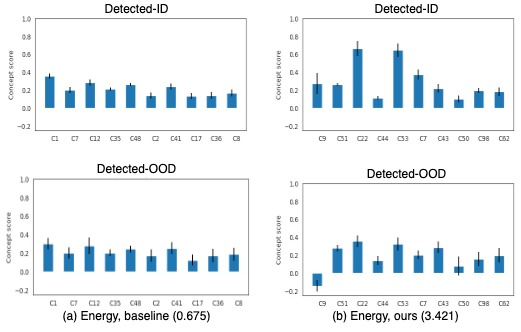
\includegraphics[width=0.8\linewidth]{figures/visual_dstinct.jpg}
  \captionof{figure}{
\small \textbf{Concept separability and visual distinction in the concept score patterns.} For the class "Giraffe", we compare the concept score patterns using two different sets of concepts. \textbf{Left:} Averaged scores of top-10 important concepts out of the concepts learned by ~\cite{yeh2020completeness}). 
\textbf{Right:} Averaged scores of top-10 important concepts out of the concepts learned by our method ($\,\lambda_\textrm{mse} = 1, \lambda_\textrm{norm} = 0.1, \lambda_\textrm{sep} = 50$ with Energy detector).
Concept importance is measured using the Shapley value of Eqn. (\ref{equ: ConceptSHAP}).
% For visualization of what each concept represents, see Appendix.
% C$i$ denotes $i$-th concept.
}
\label{fig:separa_interpretatbility}
\end{figure}

% Lastly, we use the concepts to gain insights on OOD detectors.
% We investigate whether the concepts with a higher concept-separability measure lead to a more distinguishable pattern 
%in the concept scores between detected-ID inputs and detected-OOD inputs. 
% between the concept scores of detected-ID inputs and detected-OOD inputs.
In Fig. \ref{fig:separa_interpretatbility}, we take the average of concept scores $V_{\textrm{in}}(\bfC)$ (or $V_{\textrm{out}}(\bfC)$) among the inputs that are predicted as class $y$, and detected as ID (or OOD) by Energy detector as an example.
% where $\bfC'$ is the subset of original $m$ concepts $\bfC$. 
% Here, we constitute the subset by taking the top-10 important concepts, ranked by their SHAP($\eta^{j}_{\bff, S}(\bfC)$) scores.
% By comparing the patterns of averaged concept scores, one can understand how ID-detected inputs and OOD-detected inputs are different in terms of concepts, even when predicted to same class (compare Figure \ref{fig:low_in} vs. Figure \ref{fig:low_out}, or Figure \ref{fig:high_in} vs. Figure \ref{fig:high_out}).
We can observe noticeably distinguishable pattern between detected-ID and detected-OOD concept scores when using concepts with higher concept separability ($J_{\textrm{sep}}(\bfC, \bfC')=3.421$), compared to those of low concept separability ($J_{\textrm{sep}}(\bfC, \bfC')=0.675$) by ~\cite{yeh2020completeness}. 
These observations confirm our design motivation for the concept separability metric -- that a higher value of the concept separability metric enables better \textit{visual distinction} between the concept score patterns, suggesting better interpretability for humans.
%This suggests that as long as classification completeness and detection completeness are preserved, having higher concept separability is beneficial for better interpretability for humans. 
% For further discussion, see Appendix \ref{sec:appendix-separability}.
\fi

\section{Implementation Details}
\label{sec:appendix-implementation-details}
% In this section, we provide more details about our experiment setting.
We ran all our experiments with Tensorflow, Keras and NVDIA GeForce RTX 2080Ti GPUs. We used test-set bootstrapping with 200 runs to obtain the confidence interval for each hyperparameter setting of concept learning.

\subsection{Experimental Setting.}
\mypara{OOD Datasets.}
For the auxiliary OOD dataset for concept learning ($\Douttr$), we use the unlabeled images from MSCOCO dataset (120K images in total) \cite{lin2014mscoco}. We carefully curate the dataset to make sure that no images contain overlapping animal objects with our ID dataset (\ie 50 animal classes of Animals-with-Attributes \cite{xian2018awa}), then randomly sample 30K images.
For OOD datasets for evaluation ($\Doutte$), we use the high-resolution image datasets processed by Huang and Li~\cite{Huang_MOS}.

\mypara{Hyperparameters for Concept Learning.}
Throughout the experiments, we fix the number of concepts to $m = 100$ (unless specifically mentioned otherwise), and following the implementation of \cite{yeh2020completeness}, we set $\lambda_{\textrm{expl}} = 10$ and $\bfg$ to be a two-layer fully-connected neural network with $500$ neurons in the hidden layer.
We learn concepts based on feature representations from the layer right before the global max-pooling layer of the Inception-V3 model.
% We set the range of $\lambda_{\textrm{norm}}, \lambda_{\textrm{mse}}$ and $\lambda_{\textrm{sep}}$ (in Eqn. (\ref{equ: concept learning})) based on the scale of corresponding regularization terms (\ie $J_{\textrm{norm}}(\bfC, \bfg),  J_{\textrm{mse}}(\bfC, \bfg)$ and $ J_{\textrm{sep}}(\bfC)$, respectively), for a specific choice of the OOD detector.
% For ablation study to illustrate the effect of each parameter, see Appendix \ref{sec:appendix-concept-learning-ablation}.
After concept learning with $m$ concepts, we remove any duplicate (redundant) concept vectors by removing those with a dot product larger than $0.95$ with the remaining concept vectors~\cite{yeh2020completeness}.


\subsection{Additional Results on the Effectiveness of Our Concept Learning}
\label{sec:app_addi_results}

\mypara{Ablation Study for Concept Learning.}
\label{sec:appendix-concept-learning-ablation}
We perform an ablation study that isolates the effect of each regularization term in our concept learning objective (Eqn. \ref{equ: concept learning}) towards our evaluation metrics: classification completeness, detection completeness, and relative concept separability. 
We also observe the coherency among the learned concepts by varying $\lambda_\textrm{mse}$ and $\lambda_\textrm{sep}$.
Coherency of concepts was introduced by Ghorbani \etal~\cite{ghorbani2019ace} to ensure that the generated concept-based explanations are understandable to humans. 
It captures the idea that the examples for a concept should be similar to each other, while being different from the examples corresponding to other concepts.
For the specific case of the image domain, the receptive fields most correlated to a concept $i$ (\eg "stripe pattern") should look different from the receptive fields for a different concept $j$ (\eg "wavy surface of sea").
\citet{yeh2020completeness} proposed to quantify the coherency of concepts as 
\begin{equation}
\label{eq:coherency}
    \frac{1}{m\,K} \mysum_{i=1}^m \mysum_{\bfx^\prime \in T_{\bfc_i}} \langle \bfphi(\bfx^\prime), \bfc_i \rangle,
\end{equation}
where $T_{\bfc_i}$ is the set of $K$-nearest neighbor patches of the concept vector $\bfc_i$ from the ID training set $\Dintr$.

\begin{figure*}[hbt]
  \centering
  \begin{subfigure}{0.45\linewidth}
    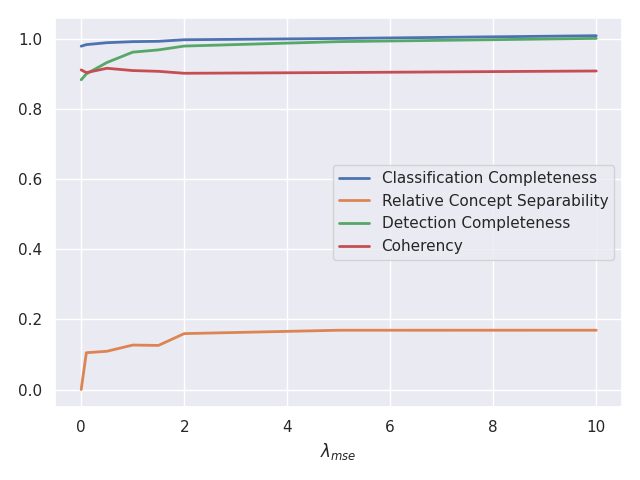
\includegraphics[width=\textwidth]{figures/ablation_mse.png}
    \caption{Ablation study varying $\lambda_\textrm{mse}$; we set $\lambda_\textrm{norm} = 0.1, \lambda_\textrm{sep} = 0$}
    \label{fig:ablation_mse}
  \end{subfigure}
  \hfill
  \begin{subfigure}{0.45\linewidth}
    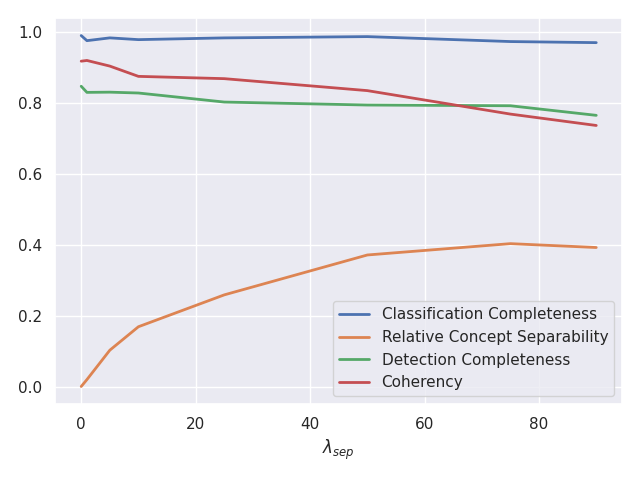
\includegraphics[width=\textwidth]{figures/ablation_sep.png}
    \caption{Ablation study varying $\lambda_\textrm{sep}$; we set $\lambda_\textrm{mse} = 0, \lambda_\textrm{norm} = 0$.}
    \label{fig:ablation_sep}
  \end{subfigure}
  \caption{\textbf{Ablation study with respect to $J_\textrm{mse}(\bfC, \bfg)$ and $J_\textrm{sep}(\bfC)$.} We fix $m = 100, \lambda_\textrm{expl} = 10$, and the OOD detector used for concept learing and evaluation is Energy \cite{liu2020energy}}
\label{fig:ablation}
\end{figure*}

We use this metric to quantify how understandable our concepts are for different hyperparameter choices. Figure~\ref{fig:ablation} shows that aligned with our intuition, large $\lambda_\textrm{mse}$ helps to improve the detection completeness. 
Having non-zero $\lambda_\textrm{mse}$ is also helpful to improve the classification completeness even further, and surprisingly concept separability as well, without sacrificing the coherency of concepts.
On the other hand, on the right side of Figure~\ref{fig:ablation}, we observe that large relative concept separability with large $\lambda_\textrm{sep}$ comes at the expense of lower detection completeness and coherency. 
Recall that when visualizing what each concept represents for human's convenience, we apply threshold 0.8 to only presents (see Figure \ref{fig:app-shap}). 
Low coherency with respect to Eqn. \ref{eq:coherency} (\ie 0.768 with $\lambda_\textrm{sep} = 75)$ means that there is much less number of examples that can pass the threshold, meaning that users can hardly understand what the concepts at hand entail.
This observation suggests that one needs to balance between concept coherency and concept separability depending on which property would be more useful for a specific application of concepts.


\mypara{Effectiveness of the Concept Learning.}
In Table~\ref{tab:concept-learning-results}, we present the complete results of concept learning for various combinations of the regularization coefficients across various real-world, large-scale OOD data: \texttt{Places}, \texttt{SUN} and \texttt{Textures}.

\begin{table*}[htb]
    \centering
    % \begin{adjustbox}{width=1\columnwidth,center}
    \begin{adjustbox}{width=1\textwidth,center}
		\begin{tabular}{l|l|l|c|c|c|c|c|c}
			\toprule
			\multirow{3}{0.001\linewidth}{OOD detector} & \multirow{3}{0.10\linewidth}{Hyper-\\parameters} &
			\multirow{3}{0.05\linewidth}{ $\eta^{}_{\bff}(\bfC) \uparrow$} & \multicolumn{6}{c}{Test OOD dataset} \\ \cline{4-9}
    		& & & \multicolumn{2}{c|}{\texttt{Places}} & \multicolumn{2}{c|}{\texttt{SUN}} & \multicolumn{2}{c}{\texttt{Textures}}\\ \cline{4-9}
    		& & & $\eta^{}_{\bff, S}(\bfC) \uparrow$ & $J_{\textrm{sep}}(\bfC, \bfC') \uparrow$ & $\eta^{}_{\bff, S}(\bfC) \uparrow$ & $J_{\textrm{sep}}(\bfC, \bfC') \uparrow$ & $\eta^{}_{\bff, S}(\bfC) \uparrow$ & $J_{\textrm{sep}}(\bfC, \bfC') \uparrow$ \\ \hline \hline
			%
            \multirow{4}{0.10\linewidth}{MSP} 
			& $(0, 0, 0)$ & 0.977 $\pm$ 0.0006 & 0.774 $\pm$ 0.0010 & 0.694 $\pm$ 0.0153 & 0.782 $\pm$ 0.0010 & 1.088 $\pm$ 0.0175 & 0.593 $\pm$ 0.0013 & 0.765 $\pm$ 0.0157\\
			& $(10, 0.1, 0)$ & \textbf{0.994} $\pm$ 0.0004 & \underline{0.947} $\pm$ 0.0004 & 1.892 $\pm$ 0.0393 & \underline{0.946} $\pm$ 0.0004 & 3.074 $\pm$ 0.0531 & \underline{0.920} $\pm$ 0.0005 & \underline{3.577} $\pm$ 0.1292\\
			& $(0, 0, 50)$ & 0.980 $\pm$ 0.0005 & 0.814 $\pm$ 0.0008 & \underline{2.533} $\pm$ 0.0714 & 0.816 $\pm$ 0.0009 & \underline{4.295} $\pm$ 0.1048 & 0.773 $\pm$ 0.0010 & 3.147 $\pm$ 0.2076\\
			& $(10, 0.1, 50)$ & \underline{0.984} $\pm$ 0.0004 & \textbf{0.960} $\pm$ 0.0004 & \textbf{2.756} $\pm$ 0.0854 & \textbf{0.961} $\pm$ 0.0005 & \textbf{4.442} $\pm$ 0.0830 & \textbf{0.937} $\pm$ 0.0004 & \textbf{3.587} $\pm$ 0.2145\\ \hline
			%
            \multirow{4}{0.10\linewidth}{ODIN} 
			& $(0, 0, 0)$ & 0.977 $\pm$ 0.0006 & 0.742 $\pm$ 0.0011 & 0.444 $\pm$ 0.0119 & 0.745 $\pm$ 0.0010 & 0.710 $\pm$ 0.0156 & 0.618 $\pm$ 0.0013 & 0.501 $\pm$ 0.0121 \\
			& $(10^8, 0.1, 0)$ & \textbf{0.994} $\pm$ 0.0004 & \underline{0.951} $\pm$ 0.0004 & 1.166 $\pm$ 0.0303 & \underline{0.958} $\pm$ 0.0004 & 2.135 $\pm$ 0.0450 & \underline{0.934} $\pm$ 0.0004 & 2.793 $\pm$ 0.0865\\
			& $(0, 0, 50)$ & 0.987 $\pm$ 0.0004 & 0.899 $\pm$ 0.0007 & \underline{1.785} $\pm$ 0.0669 & 0.911 $\pm$ 0.0006 & \underline{3.814} $\pm$ 0.0768 & 0.793 $\pm$ 0.0008 & \underline{3.046} $\pm$ 0.2845\\
			& $(10^8, 0.1, 50)$ & \underline{0.991} $\pm$ 0,0005 & \textbf{0.973} $\pm$ 0.0009 & \textbf{1.813} $\pm$ 0.0268 & \textbf{0.969} $\pm$ 0.0010 & \textbf{4.000} $\pm$ 0.0094 & \textbf{0.945} $\pm$ 0.0006 & \textbf{3.662} $\pm$ 0.1005\\ \hline
			%
            \multirow{4}{0.10\linewidth}{General-ODIN} 
			& $(0, 0, 0)$ & 0.988 $\pm$ 0.0004 & 0.769 $\pm$ 0.0004 & 0.506 $\pm$ 0.0165 & 0.719 $\pm$ 0.0014 & 0.816 $\pm$ 0.0192 & 0.605 $\pm$ 0.0013 & 0.558 $\pm$ 0.1683\\
			& $(10^6, 0.1, 0)$ & \textbf{0.995} $\pm$ 0.0004 & \underline{0.951} $\pm$ 0.0006 & 1.461 $\pm$ 0.0321 & \underline{0.960} $\pm$ 0.0005 & 3.007 $\pm$ 0.0316 & \underline{0.940} $\pm$ 0.0008 & 2.619 $\pm$ 0.1077\\
			& $(0, 0, 50)$ & 0.981 $\pm$ 0.0004 & 0.859 $\pm$ 0.0007 & \underline{1.814} $\pm$ 0.0685 & 0.803 $\pm$ 0.0006 & \underline{4.204} $\pm$ 0.0159 & 0.826 $\pm$ 0.0008 & \textbf{4.014} $\pm$ 0.2246\\
			& $(10^6, 0.1, 50)$ & \underline{0.990} $\pm$ 0.0005 & \textbf{0.971} $\pm$ 0.0010 & \textbf{1.835} $\pm$ 0.0669 & \textbf{0.963}$\pm$ 0.0004 & \textbf{4.287} $\pm$ 0.0284 & \textbf{0.951} $\pm$ 0.0005 & \underline{3.695} $\pm$ 0.1921 \\ \hline
			%
            \multirow{4}{0.10\linewidth}{Energy} 
			& $(0, 0, 0)$ & 0.977 $\pm$ 0.0006 & 0.671 $\pm$ 0.0012 & 0.453 $\pm$ 0.0121 & 0.682 $\pm$ 0.0012 & 0.675 $\pm$ 0.0148 & 0.557 $\pm$ 0.0014 & 0.521 $\pm$ 0.0131\\
			& $(1. 0.1, 0)$ & \textbf{0.993} $\pm$ 0.0005 & \textbf{0.965} $\pm$ 0.0004 & 1.266 $\pm$ 0.0319 & \textbf{0.963} $\pm$ 0.0004 & 2.125 $\pm$ 0.0413 & \textbf{0.960} $\pm$ 0.0003 & 2.648 $\pm$ 0.0596\\
			& $(0, 0, 50)$ & \underline{0.987} $\pm$ 0.0005 & 0.779 $\pm$ 0.0010 & \textbf{1.920} $\pm$ 0.0725 & 0.793 $\pm$ 0.0009 & \textbf{3.659} $\pm$ 0.0659 & 0.767 $\pm$ 0.0010 & \textbf{4.397} $\pm$ 0.2165 \\
			& $(1, 0.1, 50)$ & 0.980 $\pm$ 0.0005 & \underline{0.943} $\pm$ 0.0005 & \underline{1.839} $\pm$ 0.0662 & \underline{0.941} $\pm$ 0.0005 & \underline{3.421} $\pm$ 0.0619 & \underline{0.936} $\pm$ 0.0005 & \underline{3.917} $\pm$ 0.1691 \\ \hline
			%
			\multirow{4}{0.10\linewidth}{Mahala-\\nobis} 
			& $(0, 0, 0)$ & 0.990 $\pm$ 0.0007 & 0.715 $\pm$ 0.0011 & 0.571 $\pm$ 0.0110 & 0.736 $\pm$ 0.0011 & 0.822 $\pm$ 0.0165 & 0.591 $\pm$ 0.0011 & 0.564 $\pm$ 0.0203 \\
			& $(0.1, 0.1, 0)$ & \textbf{0.994} $\pm$ 0.0004 & \underline{0.950} $\pm$ 0.0009 & 1.532 $\pm$ 0.0351 & \underline{0.960} $\pm$ 0.0010 & 2.276 $\pm$ 0.0466 & \underline{0.938} $\pm$ 0.0004 & 2.915 $\pm$ 0.1132\\
			& $(0, 0, 50)$ & 0.985 $\pm$ 0.0004 & 0.880 $\pm$ 0.0005 & \underline{2.550} $\pm$ 0.0681 & 0.883 $\pm$ 0.0006 & \underline{4.091} $\pm$ 0.1013 & 0.774 $\pm$ 0.0007 & \underline{4.274} $\pm$ 0.2305\\
			& $(0.1, 0.1, 50)$ & \underline{0.992} $\pm$ 0.0006 & \textbf{0.961} $\pm$ 0.0005 & \textbf{2.616} $\pm$ 0.0857 & \textbf{0.966} $\pm$ 0.0005 & \textbf{4.325} $\pm$ 0.0055 & \textbf{0.949} $\pm$ 0.0003 & \textbf{4.308} $\pm$ 0.2011 \\ \bottomrule
		\end{tabular}
	\end{adjustbox}
	\caption[]{
	\small \textbf{Results of concept learning with different parameter settings across various OOD detectors and test OOD datasets.} 
% 	$\bfC'$ denotes a set of concepts discovered by baseline \citep{yeh2020completeness} (\ie $\lambda_\textrm{mse} = 0, \lambda_\textrm{norm} = 0, \lambda_\textrm{sep} = 0$).
	Hyperparameters are in the order of $(\lambda_\textrm{mse}, \lambda_\textrm{norm}, \lambda_\textrm{sep})$.
% 	Larger values are better for all the metrics. 
	Across the rows (for a given OOD detector and OOD dataset), the best value is \textbf{boldfaced}, and second best value is \underline{underscored}.
	The $95\%$ confidence intervals are estimated by bootstrapping the test set over $200$ trials.}
% 	\textbf{Bold} numbers indicate the best results (across the rows) for a given OOD detection method and dataset. 
	%Note that by definition of $J_{\textrm{sep}}(\bfC, \bfC')$ (Eqn. \ref{eq:relative-separability}), the relative concept separability of the baseline~\citep{yeh2020completeness} is always $0$, \ie $J_{\textrm{sep}}(\bfC', \bfC') = 0$.
 \label{tab:concept-learning-results}
% \vspace{-.2in}
\end{table*}



\mypara{Accurate Reconstruction of OOD Scores}
In addition to Fig.~\ref{fig:score-distribution-msp}, where we compared the reconstruction accuracy of OOD scores using concepts by \citet{yeh2020completeness} and ours, Fig.~\ref{fig:score-distribution-energy} confirms that the same observation also applies to the Energy detector.

\begin{figure*}
  \centering
  \begin{subfigure}{0.32\linewidth}
    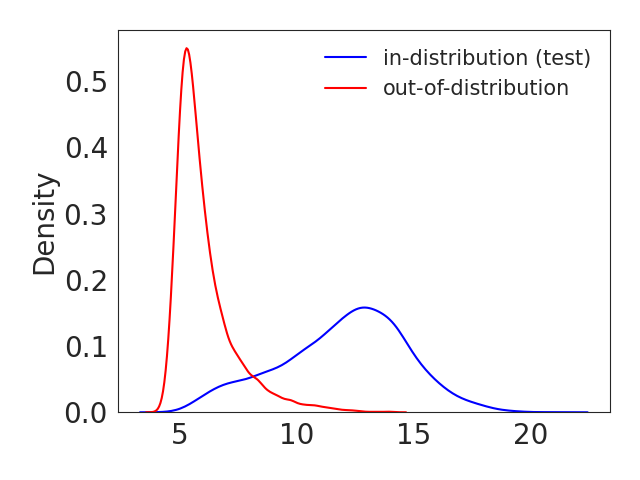
\includegraphics[width=\textwidth]{figures/distr_energy_target.png}
    \caption{\small Empirical distribution of $S(\bfx, \bff)$ from the target detector.}
    \label{fig:short-a1}
  \end{subfigure}
  \hfill
  \begin{subfigure}{0.32\linewidth}
    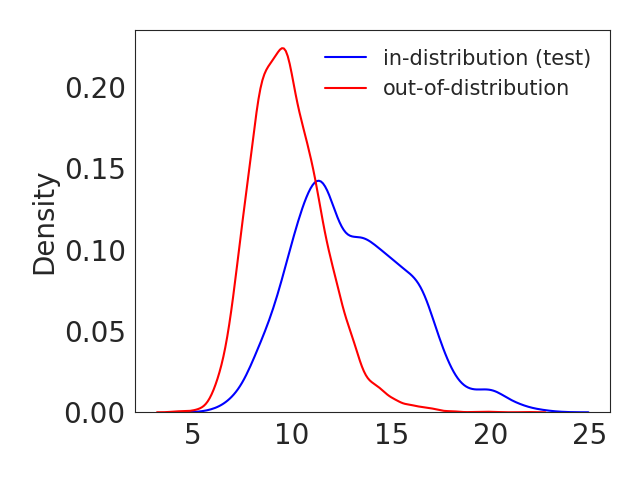
\includegraphics[width=\textwidth]{figures/distr_energy_yeh.png}
    \caption{\small Distribution of $\Scon(\bfx, \bff)$ using concepts learned by \citet{yeh2020completeness}.}
    \label{fig:short-b1}
  \end{subfigure}
  \hfill
  \begin{subfigure}{0.32\linewidth}
    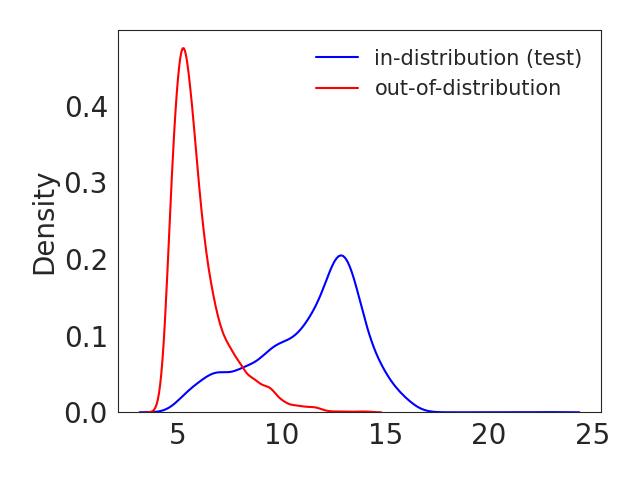
\includegraphics[width=\textwidth]{figures/distr_energy_ours.png}
    \caption{\small Distribution of $\Scon(\bfx, \bff)$ using concepts learned by our method.}
    \label{fig:short-c1}
  \end{subfigure}
  \caption{
  \small (a) Energy detector score $S(\bfx, \bff)$ in the canonical world vs. (b, c) reconstructed $\Scon(\bfx, \bff)$ in the concept world, using different set of concepts.
  Concepts by~\citet{yeh2020completeness} have $\eta^{}_{\bff} = 0.977, ~\eta^{}_{\bff, S}(\bfC) = 0.682$, while concepts by ours $(\lambda_\textrm{mse} = 1, \lambda_\textrm{norm} = 0.1, \lambda_\textrm{sep} = 50)$ have $\eta^{}_{\bff} = 0.984, ~\eta^{}_{\bff, S}(\bfC) = 0.941$.
    Comparison is made between AwA test set (ID, blue) vs. \texttt{SUN} (OOD, red).
    }
\label{fig:score-distribution-energy}
\end{figure*}

\iffalse
\mypara{Transferability of concepts across OOD detectors.}
\label{sec:appendix-concept-learning-transfer}
Our work essentially suggests using a different set of concepts for a specific target OOD detector, as $J_{\textrm{mse}}(\bfC, \bfg)$ and $J_{\textrm{sep}}(\bfC)$ in Eqn. (\ref{equ: concept learning}) depend on a choice of OOD detector. 
In practice, however, one might not have enough computational capacity to prepare multiple sets of concepts for all type of OOD detectors at hand.
Here, we inspect whether the concepts targeted for a certain type of OOD detector are also good to be used for other OOD detectors.
% For instance, 
% $J_\textrm{sep}(\bfC, \bfC') = 0.494$
% But interestingly, relative concept separability tends to be transferred well.
% For full transferability results of concepts targeted for different type of OOD detectors, and tested with different OOD data, see Appendix \ref{sec:appendix-concept-learning-transfer}.

We explore the transferability of concepts targeted to MSP \cite{hendrycks2016msp} detector in Table \ref{tab:transferability-msp}, and Energy \cite{liu2020energy} in Table \ref{tab:transferability-energy}.
Not surprisingly, we observe that concepts targeted for Energy yields the best detection completeness score when tested with the same type of OOD detector, but still make meaningful improvement with other detectors as well.
When it comes to relative concept separability, it is transferred even better across different OOD detectors. 
For instance, the concepts lead to $J_\textrm{sep}(\bfC, \bfC') = 0.862$ with \texttt{Textures}, the best relative concept separability is achieved with ODIN detector (\ie $J_\textrm{sep}(\bfC, \bfC') = 0.862$) and which is even higher than the best results we could obtain using the set of concepts targeted for ODIN (\ie $J_\textrm{sep}(\bfC, \bfC') = 0.414$ with $\lambda_\textrm{mse} = 0, \lambda_\textrm{norm} = 0, \lambda_\textrm{sep} = 50$ in Table \ref{tab:concept-learning-results}).
\begin{table*}[htb]
    % \centering
    % \begin{adjustbox}{}
\begin{subtable}{.47\linewidth}
\begin{adjustbox}{width=\textwidth,center}
\begin{tabular}{l|l|c|c|c|c}
			\toprule
			\multirow{2}{0.35\linewidth}{OOD dataset} & \multirow{2}{0.06\linewidth}{Metrics} & \multicolumn{4}{c}{$\calD$} \\ \cline{3-6}
    		& & MSP & ODIN & Energy & Mahal\\  \hline \hline
    % 		& & & $\mu_{f, \calD} (\bfC)$ & S(\bfC) & $\mu_{f, \calD} (\bfC)$ & S(\bfC) & $\mu_{f, \calD} (\bfC)$ & S(\bfC) & $\mu_{f, \calD} (\bfC)$ & S(\bfC) \\ \hline \hline
			\multirow{2}{0.08\linewidth}{\texttt{Places}} & $\eta^{}_{\bff, S}(\bfC)$ & 0.959 & 0.952 & 0.938 & 0.947\\ 
			& $J_{\textrm{sep}}(\bfC, \bfC')$ & 0.327 & 0.288 & 0.361 & 0.338 \\\hline 
            \multirow{2}{0.08\linewidth}{\texttt{SUN}} & $\eta^{}_{\bff, S}(\bfC)$ & 0.961 & 0.954 & 0.945 & 0.953 \\ 
			& $J_{\textrm{sep}}(\bfC, \bfC')$ & 0.266 & 0.294 & 0.390 & 0.351\\\hline 
			\multirow{2}{0.08\linewidth}{\texttt{Textures}} & $\eta^{}_{\bff, S}(\bfC)$ & 0.938 & 0.946 & 0.932 & 0.930\\ 
			& $J_{\textrm{sep}}(\bfC, \bfC')$ & 0.344 & 0.279 & 0.313 & 0.335\\\hline 
			\multirow{2}{0.08\linewidth}{\texttt{iNaturalist}} & $\eta^{}_{\bff, S}(\bfC)$ & 0.946 & 0.946 & 0.933 & 0.930\\ 
			& $J_{\textrm{sep}}(\bfC, \bfC')$ & 0.286 & 0.181 & 0.229 & 0.197\\
 \bottomrule
    \end{tabular}
    \end{adjustbox}
        \caption[]{Concepts targeted for MSP with $\lambda_\textrm{mse} = 10, \lambda_\textrm{norm} = 0.1, \lambda_\textrm{sep} = 50$}
    \label{tab:transferability-msp}
        \end{subtable}
 % \hfill
     % \small
    % \centering
    \hspace{\fill}
\begin{subtable}{.47\linewidth}
\begin{adjustbox}{width=\textwidth,center}

		\begin{tabular}{l|l|c|c|c|c}
			\toprule
			\multirow{2}{0.35\linewidth}{OOD data} & \multirow{2}{0.06\linewidth}{Metrics} & \multicolumn{4}{c}{OOD detector} \\ \cline{3-6}
    		& & MSP & ODIN & Energy & Mahal\\  \hline \hline
    % 		& & & $\mu_{f, \calD} (\bfC)$ & S(\bfC) & $\mu_{f, \calD} (\bfC)$ & S(\bfC) & $\mu_{f, \calD} (\bfC)$ & S(\bfC) & $\mu_{f, \calD} (\bfC)$ & S(\bfC) \\ \hline \hline
			\multirow{2}{0.08\linewidth}{\texttt{Places}} & $\eta^{}_{\bff, S}(\bfC)$ &0.956& 0.954 &0.971 & 0.954\\ 
			& $J_{\textrm{sep}}(\bfC, \bfC')$ & 0.417 & 0.415 &0.365& 0.410 \\\hline 
            \multirow{2}{0.08\linewidth}{\texttt{SUN}} & $\eta^{}_{\bff, S}(\bfC)$ &0.949& 0.948 &0.970& 0.950\\ 
			& $J_{\textrm{sep}}(\bfC, \bfC')$ & 0.355 &0.286 &0.400& 0.353 \\\hline 
			\multirow{2}{0.08\linewidth}{\texttt{Textures}} & $\eta^{}_{\bff, S}(\bfC)$ &0.931& 0.943 &0.964& 0.947\\ 
			& $J_{\textrm{sep}}(\bfC, \bfC')$ & 0.567 & 0.862&0.494&0.701 \\\hline 
			\multirow{2}{0.08\linewidth}{\texttt{iNaturalist}} & $\eta^{}_{\bff, S}(\bfC)$ &0.943& 0.939 &0.973& 0.940\\ 
			& $J_{\textrm{sep}}(\bfC, \bfC')$ & 0.283 &0.448 &0.280& 0.326\\
 \bottomrule
		\end{tabular}
   
	\end{adjustbox}
        
        \caption[]{Concepts targeted for Energy with $\lambda_\textrm{mse} = 1, \lambda_\textrm{norm} = 0.1, \lambda_\textrm{sep} = 50$}
	\label{tab:transferability-energy}
 \end{subtable}
\caption{Transferability of concepts across different OOD detectors.}
\end{table*}

% \begin{table}[htb]

% \end{table}

\fi 


\subsection{Accurate Reconstruction of Classifier Outputs}
\label{app:hellinger}
We have performed additional experiments to understand if the proposed method can provide improvements in the classification setting. 
Let $\mathbf{C}_1$ denote the concept matrix learned by the method of \citet{yeh2020completeness}. 
Let $\mathbf{C}_2$ denote the concept matrix learned by our method with $\lambda_{mse} = \lambda_{sep} = 0$ and $\lambda_{norm} = 0.1$ (set based on the scale of the regularization term $J_{norm}$). The idea is that we exclude the terms in the concept-learning objective (Eqn.~\ref{equ: concept learning}) that depend on the OOD detector, but include the $\ell_2$ norm based reconstruction error of the layer representation. 
To evaluate the utility of these two sets of concepts for classification, we calculated the per-sample Hellinger distance between the predicted class probabilities of the original classifier and the concept-world classifier (based on either $\mathbf{C}_1$ or $\mathbf{C}_2$). 
Fig.~\ref{fig:hellinger} compares the empirical distribution of the Hellinger distance for both sets of concepts $\mathbf{C}_1$ and $\mathbf{C}_2$. We observe that the distribution is more skewed towards zero with a higher density near zero and a shorter (right) tail in the case of $\mathbf{C}_2$ (red curve) compared to $\mathbf{C}_1$ (blue curve). This suggests that the class predictions are more accurately reconstructed by the concepts learned using our method with only the reconstruction error-based regularization. This can in-turn benefit the concept-based explanations for the classifier.

\begin{figure*}[t]
  \centering
  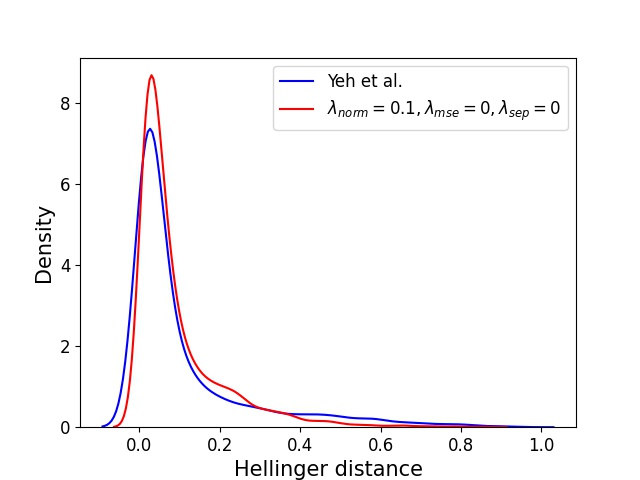
\includegraphics[width=0.5\textwidth]{figures/classification_hellinger.jpg}
\caption{Examples for correct detection}
\label{fig:hellinger}
\end{figure*}


\iffalse

\subsection{Separability in explanations}
\label{sec:appendix-separability}
% Let $X_{in}$ be the set of data detected as ID by $\mathcal{D}$. That is, $\mathcal{D(\bfx)} \geq \tau, ~ \forall \bfx \in X_{in}$. And $X_{out}$ be the set of data detected as OOD by $\mathcal{D}$: $\mathcal{D(\bfx)} < \tau, ~\forall \bfx \in X_{out}$.

% \begin{equation}
%     CAV_{in} = \frac{\sum_{\bfx_i \in X_{in}} v_\bfC(\bfx_i)}{|X_{in}|}
% \end{equation}
% \begin{equation}
%     \label{equ: CAV}
%     CAV_{out} = \frac{\sum_{\bfx_i \in X_{out}} v_\bfC(\bfx_i)}{|X_{out}|}
% \end{equation}

% AwA vs SUN
\begin{figure}[h]
\centering
\subfloat[ID, baseline \label{fig:yeh_low_separa_in}]{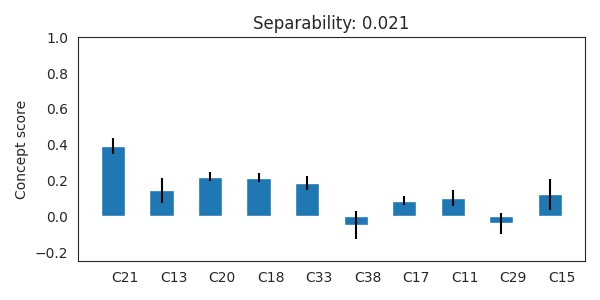
\includegraphics[width=0.5\textwidth]{yeh_class15_AwA2_top10_detected_Energy.jpg}}\hfill
\subfloat[ID, ours \label{fig:ours_low_separa_in}] {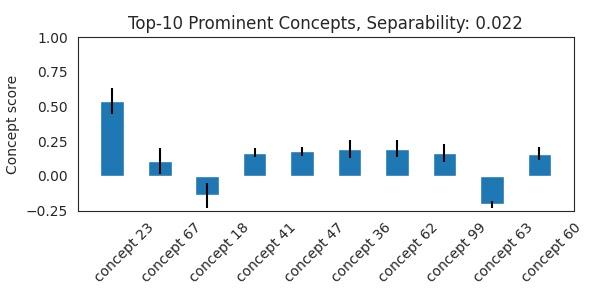
\includegraphics[width=0.5\textwidth]{figures/ours_class15_AwA2_top10_detected_Energy.jpg}}\hfill\\
\subfloat[OOD, baseline\label{fig:yeh_low_separa_out}]{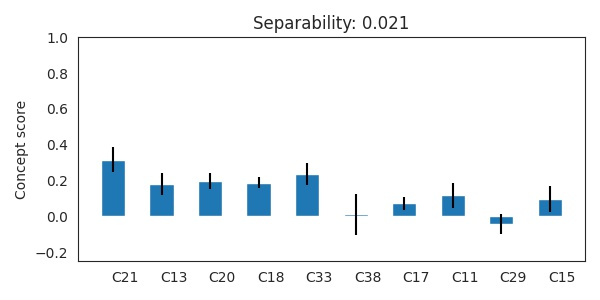
\includegraphics[width=0.5\textwidth]{figures/yeh_class15_SUN_top10_detected_Energy.jpg}}\hfill
\subfloat[OOD, ours \label{fig:ours_low_separa_out}] {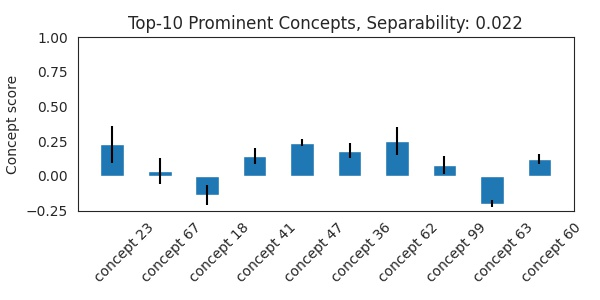
\includegraphics[width=0.5\textwidth]{figures/ours_class15_SUN_top10_detected_Energy.jpg}}
\caption{Easy class ("German Shepherd") with lowest separability. Top-10 concepts with highest conceptSHAP score}
\label{fig:high_separa}
\end{figure}
\fi

\section{Choice of Auxiliary OOD Dataset in Concept Learning}
\label{app:auxiliary-ood}

Under circumstances where having access to auxiliary OOD dataset for concept learning is not feasible, we suggest that one could use generative methods to generate synthetic dataset, or apply data augmentation techniques. Fig.~\ref{fig:app-augAwA} shows an example of AwA image augmented by \citet{hendrycks2022pixmix}. 

\begin{figure*}[hbt]
\centering
{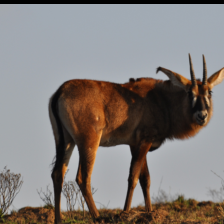
\includegraphics[width=0.2\textwidth]{figures/appendix/9_orig.png}} \hspace{2mm}
{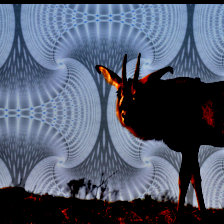
\includegraphics[width=0.2\textwidth]{figures/appendix/9.png}}
\caption{\textbf{Random example of augmented AwA dataset.} 
\textbf{Left:} original image in AwA train set.
\textbf{Right:} corresponding image augmented using the method of \citet{hendrycks2022pixmix}.} 
\label{fig:app-augAwA}
\end{figure*}

We evaluate the effectiveness of our concept learning objective when such augmented AwA train set is used as auxiliary OOD dataset.
Table~\ref{tab:app-auxiliary-ood} illustrates that the generated concepts with augmented AwA (\ie OOD data close to target ID data) have comparable detection completeness and concept separability compared to when MSCOCO (\ie OOD data far from ID data) was used.
But still, further evaluation on generated concept-based explanations with different choice of auxiliary OOD dataset remains as an interesting research question.

\begin{table}[htb]
    \centering
    \begin{adjustbox}{width=1\columnwidth,center}
		\begin{tabular}{l|l|l|c|c|c|c|c|c}
			\toprule
			\multirow{3}{0.001\linewidth}{OOD detector} & \multirow{3}{0.10\linewidth}{Hyper-\\parameters} &
			\multirow{3}{0.05\linewidth}{ $\eta^{}_{\bff}(\bfC) \uparrow$} & \multicolumn{6}{c}{Test OOD dataset} \\ \cline{4-9}
    		& & & \multicolumn{2}{c|}{\texttt{Places}} & \multicolumn{2}{c|}{\texttt{SUN}} & \multicolumn{2}{c}{\texttt{Textures}}\\ \cline{4-9}
    		& & & $\eta^{}_{\bff, S}(\bfC) \uparrow$ & $J_{\textrm{sep}}(\bfC, \bfC') \uparrow$ & $\eta^{}_{\bff, S}(\bfC) \uparrow$ & $J_{\textrm{sep}}(\bfC, \bfC') \uparrow$ & $\eta^{}_{\bff, S}(\bfC) \uparrow$ & $J_{\textrm{sep}}(\bfC, \bfC') \uparrow$ \\ \hline \hline
			%
            % {MSP} & $(10, 0.1, 50)$ & \underline{0.984} $\pm$ 0.0004 & \underline{\textbf{0.960}} $\pm$ 0.0004 & \underline{\textbf{2.756}} $\pm$ 0.0854 & \underline{\textbf{0.961}} $\pm$ 0.0005 & \underline{\textbf{4.442}} $\pm$ 0.0830 & \underline{\textbf{0.937}} $\pm$ 0.0004 & \underline{\textbf{3.587}} $\pm$ 0.2145\\ \hline

            {Energy} 
			& $(1, 0.1, 50)$ & 0.955 $\pm$ 0.0006 & 0.940 $\pm$ 0.0005 & 1.746 $\pm$ 0.0712 & 0.9410 $\pm$ 0.0005 & 3.0703 $\pm$ 0.0580 & 0.927 $\pm$ 0.0005 & 3.417 $\pm$ 0.1419 \\
			\bottomrule
		\end{tabular}
	\end{adjustbox}
        \vspace{2mm}
	\caption[]{Results of concept learning with augmented AwA train set as auxiliary OOD in concept learning.
	}
	\label{tab:app-auxiliary-ood}
\end{table}





\section{Explanations}
\label{sec:appendix-shapleys}


\iffalse
\begin{figure}[h]
% \vspace{1mm}
% \begin{center}
%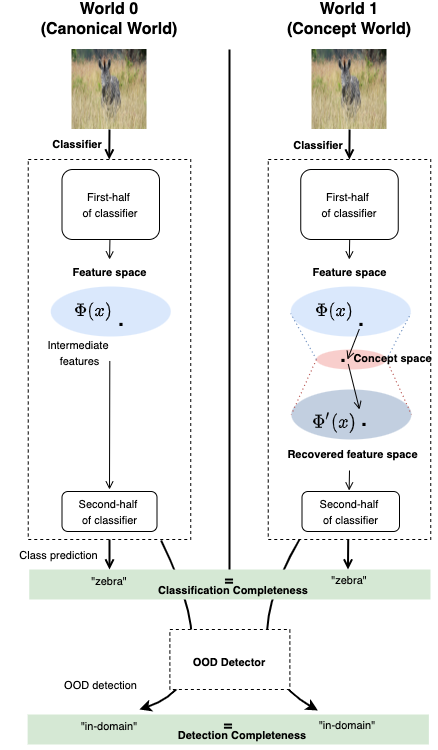
\includegraphics[width=0.45\textwidth]{figures/completeness.png}
% \hspace*{+.5cm} 
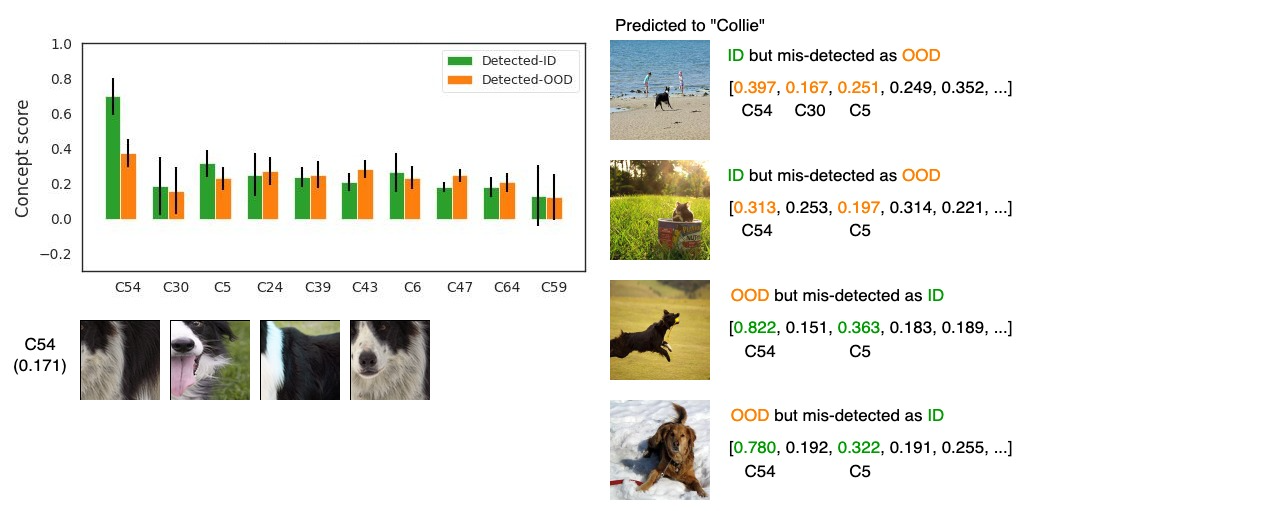
\includegraphics[scale=0.35]{figures/expl_collie.png}
% \vspace{-9mm}
\caption{
\small \textbf{Our concept-based explanations for Energy detector}~\citep{liu2020energy}. Concepts are discovered by our method with $\lambda_\textrm{mse} = 1, \lambda_\textrm{norm} = 0.1, \lambda_\textrm{sep} = 10$.}
\label{fig:expl_collie}
% \end{center}
\end{figure}
\fi

\subsection{Important Concepts for Each OOD Detector}
\label{sec:appendix-explanation}
We show additional examples for the top-ranked concepts by $\textrm{SHAP}(\eta_{\bff, S}, \bfc_i)$ in Fig. \ref{fig:app-shap}.
For each figure with a fixed choice of class prediction, we present receptive fields from ID test set corresponding to top concepts that contribute the most to the decisions of each OOD detector.
All receptive fields passed the threshold test that the inner product between the feature representation and the corresponding concept vector is over $0.85$.
\begin{figure*}[ht]
\centering
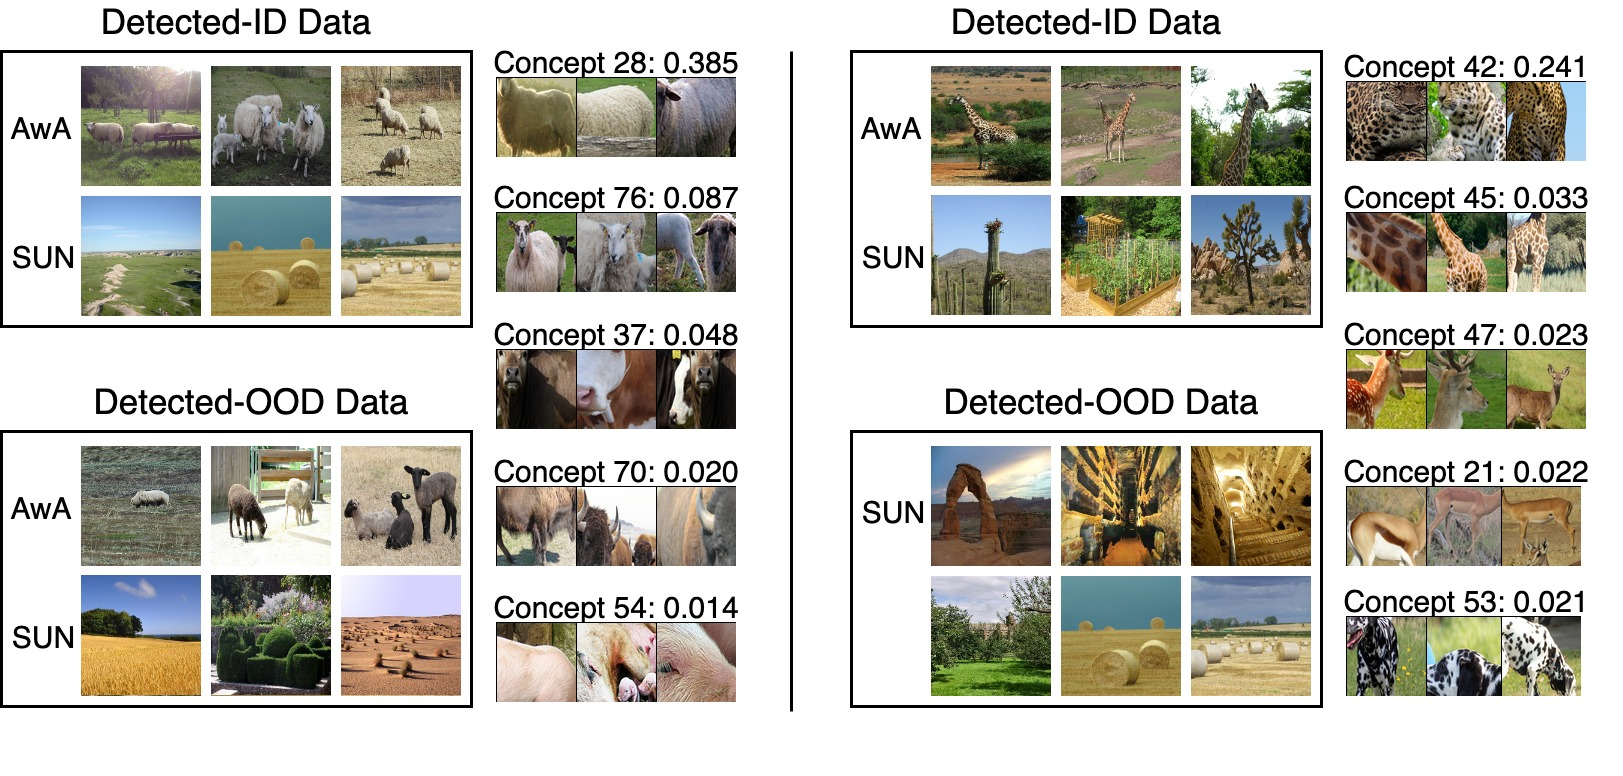
\includegraphics[width=\textwidth]{figures/concepts.jpg}
\vspace{-0.3in}
\caption{Top-6 important concepts for the Energy OOD detector with respect to class ``Sheep'' (on the left) and class ``Giraffe'' (on the right).}
\label{fig:app-shap}
\end{figure*}

Moreover, in Fig. \ref{fig:shap_buffalo}, we compare the important concepts discovered by the baseline method \cite{yeh2020completeness} (denoted as ``baseline'') vs. ours.
With the baseline, when the learned concepts are solely intended for reconstructing the behavior of the classifier, we observe that interpretation of both the classifier and OOD detector depends on a common set of concepts (\ie concepts 32, 10, and 47).
On the other hand, the concepts learned by our method focus on reconstructing the behavior of both the OOD detector and the classifier. In this case, we observe that a distinct set of important concepts are selected for classification and OOD detection.
We also observe that our method requires more concepts in order to address the decisions of both the classifier and OOD detector.
For instance, the number of concepts obtained by our method and the baseline are 78 and 53 (respectively), out of a total 100 concepts after the duplicate removal of concept vectors.
In short, when the concepts are only targeted at explaining the DNN classifier (as in the baseline \cite{yeh2020completeness}), the behavior of the OOD detector is merely described by the common set of concepts that are important for the DNN classifier.
On the other hand, when not only the DNN classifier but also the OOD detector is taken into consideration during concept learning (\ie our method), we obtain a more diverse and expanded set of concepts, and different concepts play a major role in interpreting the classification and detection results. 

\begin{figure}[hbt]
% \vspace{1mm}
\centering
%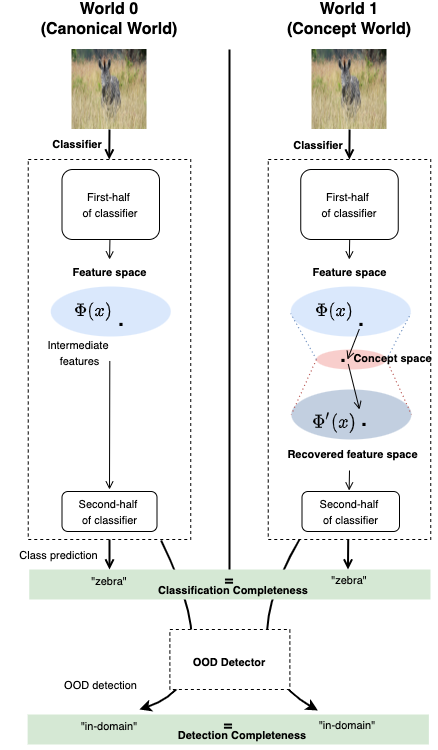
\includegraphics[width=0.45\textwidth]{figures/completeness.png}
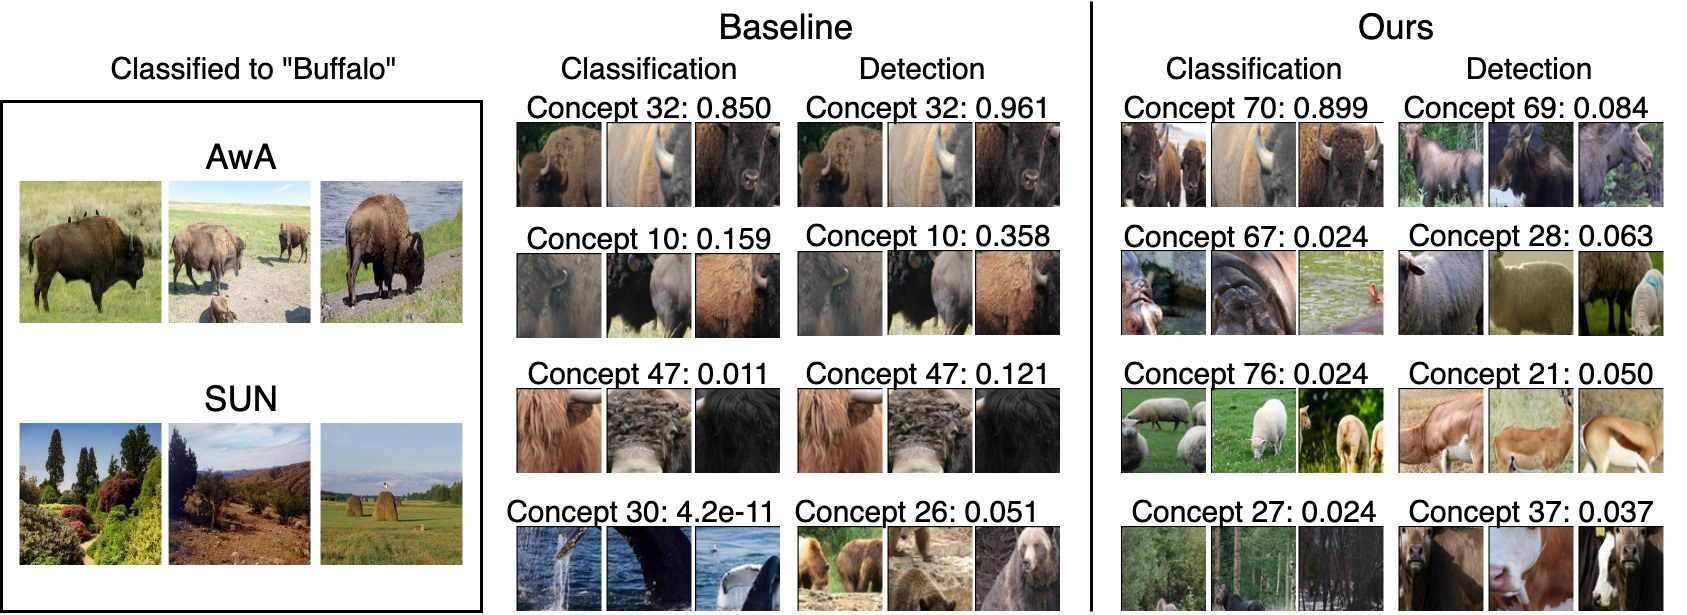
\includegraphics[width=\textwidth]{figures/expl_buffalo.jpeg}
% \vspace{-9mm}
\caption{\textbf{Most important concepts for the Energy detector with respect to the predicted class ``Buffalo''.} 
% Concepts are obtained by our concept learning algorithm with $\lambda_\textrm{mse} = 1, \lambda_\textrm{norm} = 0.1, \lambda_\textrm{sep} = 0$.
We demonstrate randomly sampled images that are predicted by the classifier into this class. 
We compare the top-4 important concepts to describe the DNN classifier (and Energy detector), ranked by the Shapley value based on classification completeness $\textrm{SHAP}(\eta^{j}_{\bff}, \bfc_i)$ (and detection completeness $\textrm{SHAP}(\eta^{j}_{\bff, S}, \bfc_i)$).
``Baseline'' corresponds to the case when the concepts are learned with $\lambda_\textrm{mse} = \lambda_\textrm{norm} = \lambda_\textrm{sep} = 0$, whereas ``Ours'' corresponds to the concepts learned with $\lambda_\textrm{mse} = 1, \lambda_\textrm{norm} = 0.1, \lambda_\textrm{sep} = 0$.
% To visualize what each concept represents, we display the top receptive fields from $\Dinte$ whose inner-product with the corresponding concept vector is larger than 0.8.
}
% \vspace{-5mm}
\label{fig:shap_buffalo}
\end{figure}

\subsection{More Examples of Our Concept-Based Explanation}
\label{app:more-expl}
In Fig.~\ref{fig:expl-additional1}, we provide additional examples of the concept-based explanations provided by  our method and compare it with that of \cite{yeh2020completeness}.

% \textcolor{blue}{Needs a couple of lines about the takeaway message.}



\begin{figure*}[b]
  \centering
  \begin{subfigure}{\linewidth}
    \includegraphics[width=\textwidth]{figures/energy_SUN_Collie.jpg}
    \caption{class ``Collie'', Energy OOD detector. Images randomly selected from AwA test set and \texttt{SUN}.}
    % \label{fig:expl-energy-collie}
  \end{subfigure}
  \\
  \begin{subfigure}{\linewidth}
    \includegraphics[width=\textwidth]{figures/MSP_SUN_Collie.jpg}
    \caption{class ``Collie'', MSP OOD detector. Images randomly selected from AwA test set and \texttt{SUN}.}
    % \label{fig:expl-energy-collie}
  \end{subfigure}
  % \vspace{.1in}
  % \caption{\textcolor{blue}{\textbf{Concept-based explanations using concepts by Yeh et al. vs. ours.} 
    % ID profile shows the concept-score patterns for normal ID images.}}
\label{fig:expl-additional}
\end{figure*}
  
\begin{figure*}\ContinuedFloat
  \centering
  \begin{subfigure}{\linewidth}
    \includegraphics[width=\textwidth]{figures/energy-dolphin.jpg}
    \caption{class ``Dolphin'', Energy OOD detector. Images randomly selected from AwA test set and \texttt{Places}.}
    \label{fig:expl-energy-dolphin}
  \end{subfigure}
  \\
  \begin{subfigure}{\linewidth}
    \includegraphics[width=\textwidth]{figures/MSP_Places_Dolphin.jpg}
    \caption{class ``Dolphin'', MSP OOD detector. Images randomly selected from AwA test set and \texttt{Places}.}
    \label{fig:expl-msp-dolphin}
  \end{subfigure}
  \vspace{.1in}
  \caption{\textbf{Concept-based explanations using concepts identified by \citet{yeh2020completeness} vs. ours.}
ID profile shows the average concept-score pattern for normal ID images.}
\label{fig:expl-additional1}
\end{figure*}

\iffalse
\newpage
\subsection{Counterfactual Analysis}
\label{sec:appendix-counterfactual}
% To further verify the contribution of concepts quantified by Eqn. (\ref{equ: ConceptSHAP}), we conduct counterfactual analysis, addressing the following questions: \textit{if the input had these concepts as a dominant features, would it have been detected as ID (or OOD)?}

%
\begin{wrapfigure}{r}{0.5\linewidth}
% \begin{figure}[t]
% \vspace{-10mm}
\centering
%\includegraphics[width=0.45\textwidth]{figures/completeness.png}
\includegraphics[scale=0.4]{figures/intervention_msp.png}
%\vspace{-2mm}
\caption{Performance of MSP with test-time interventions on concept scoress.}
% \vspace{-5mm}
\label{fig:intervention_msp}
\end{wrapfigure}
% \end{figure}
To verify the important concepts identified by our modified Shapley value, we perform counterfactual analysis, addressing the following question: \textit{if the OOD detector thought the input has different score for this concept, would the detection result be different?}
As we do not assume to have groundtruth annotation for concepts, we construct concept score profiles of detected-ID (or detected-OOD) inputs from held-out ID (or OOD) dataset, and refer to this as ID (or OOD) concept profile.
With the guidance of ID and OOD concept profiles, we take intervention on the concept scores of mis-detected inputs.
Specifically, for ID data mis-detected as OOD, we update their concept scores using ID profiles, and similarlly, for OOD data mis-detected as ID, their concept scores are updated with OOD profiles.
The number of concepts to be intervened can be varied.
As shown in Figure \ref{fig:intervention_msp}, with intervention on more number of important concepts (ranked by $\textrm{SHAP}(\eta^{}_{\bff, S}, \bfc_i)$)), we observe an improved performance of OOD detector in concept world.
\fi



%\printbibliography

\end{document}




